\documentclass{patmorin}
\listfiles
\usepackage{pat}
\usepackage{paralist}
\usepackage[T1]{fontenc}
\usepackage[utf8]{inputenc}
\usepackage{paralist}
\usepackage{bbm}  % needed for \mathbbm{1}
% \usepackage{logix}
\usepackage{halloweenmath}
\usepackage{stmaryrd}

\usepackage{todonotes}
\usepackage{tcolorbox}
\usepackage{booktabs}
\usepackage{multirow}
\usepackage{comment}

\usepackage{thm-restate}


% etoolbox allows for robust commands that don't need \protect, e.g.
% \newrobustcmd{\onesub}{\mathord{\includegraphics{figs/one-sub}}}
% \subsection{Approximate Voronoi Diagrams in $G^{\onesub}_k$}
\usepackage{etoolbox}

% david proposes the following additions
\renewcommand{\ge}{\geqslant}
\renewcommand{\le}{\leqslant}
\renewcommand{\geq}{\geqslant}
\renewcommand{\leq}{\leqslant}

\newcommand{\david}[1]{{\color{orange} David: #1}}
\newcommand{\vida}[1]{{\color{DarkGreen} Vida: #1}}
\newcommand{\pat}[1]{\textcolor{Blue}{Pat: #1}}
\newcommand{\gwen}[1]{\textcolor{Purple}{Gwen: #1}}
\newcommand{\piotr}[1]{\textcolor{red}{Piotr: #1}}

% \numberwithin{equation}{lem}


\newenvironment{clmproof}{\noindent\emph{Proof of Claim:}}{\hfill\rule{1ex}{1ex}}

\usepackage[longnamesfirst,numbers,sort&compress]{natbib}

\usepackage[mathlines]{lineno}
\setlength{\linenumbersep}{2em}
% \linenumbers
% \rightlinenumbers
% \linenumbers
\newcommand*\patchAmsMathEnvironmentForLineno[1]{%
 \expandafter\let\csname old#1\expandafter\endcsname\csname #1\endcsname
 \expandafter\let\csname oldend#1\expandafter\endcsname\csname end#1\endcsname
 \renewenvironment{#1}%
    {\linenomath\csname old#1\endcsname}%
    {\csname oldend#1\endcsname\endlinenomath}}%
\newcommand*\patchBothAmsMathEnvironmentsForLineno[1]{%
 \patchAmsMathEnvironmentForLineno{#1}%
 \patchAmsMathEnvironmentForLineno{#1*}}%
\AtBeginDocument{%
\patchBothAmsMathEnvironmentsForLineno{equation}%
\patchBothAmsMathEnvironmentsForLineno{align}%
\patchBothAmsMathEnvironmentsForLineno{flalign}%
\patchBothAmsMathEnvironmentsForLineno{alignat}%
\patchBothAmsMathEnvironmentsForLineno{gather}%
\patchBothAmsMathEnvironmentsForLineno{multline}%
}



% Taken from
% https://tex.stackexchange.com/questions/42726/align-but-show-one-equation-number-at-the-end
\newcommand\numberthis{\addtocounter{equation}{1}\tag{\theequation}}

\definecolor{brightmaroon}{rgb}{0.76, 0.13, 0.28}
\definecolor{linkblue}{rgb}{0, 0.337, 0.227}
\newcommand{\defin}[1]{\emph{\textcolor{brightmaroon}{#1}}}
\makeatletter
\def\mathcolor#1#{\@mathcolor{#1}}
\def\@mathcolor#1#2#3{%
  \protect\leavevmode
  \begingroup
    \color#1{#2}#3%
  \endgroup
}
\makeatother
\newcommand{\mathdefin}[1]{\mathcolor{brightmaroon}{#1}}
% \newcommand{\mathdefin}[1]{\color{brightmaroon}#1}}
\setlength{\parskip}{1ex}

% Document-specific commands and math operators
\DeclareMathOperator{\tw}{tw}
\DeclareMathOperator{\pw}{pw}
\DeclareMathOperator{\bw}{bw}
\DeclareMathOperator{\td}{td}
%\DeclareMathOperator{\rtw}{rtw}
\DeclareMathOperator{\diam}{diam}
\DeclareMathOperator{\mindist}{min-dist}
\DeclareMathOperator{\dist}{dist}
\DeclareMathOperator{\ld}{ld}
\DeclareMathOperator{\polylog}{polylog}
\DeclareMathOperator{\evol}{Evol}
\DeclareMathOperator{\ivol}{Ivol}
\DeclareMathOperator{\tvol}{Tvol}
\newcommand{\NN}{\mathbb{N}}
\newcommand{\GG}{\mathcal{G}}

\title{\MakeUppercase{\boldmath Planar graphs in blowups of fans}}

%\title{\MakeUppercase{\boldmath Planar graphs are contained in $\tilde{O}(\sqrt{n})$-blowups of fans}}

%Fan-Partitions of Planar Graphs (and Beyond)  \newline by Local Sparsification and Volume-Preserving Embeddings}}

\author{
 Vida Dujmovi{\'c}\,\footnote{School of Computer Science and Electrical Engineering, University of Ottawa, Ottawa, Canada (\texttt{vida.dujmovic@uottawa.ca}). Research supported by NSERC and a University of Ottawa Research Chair.}
 \qquad
 Gwena\"el Joret\footnote{D\'epartement d'Informatique, Universit\'e libre de Bruxelles, Belgium ({\tt gwenael.joret@ulb.be}). G.\ Joret is supported by the Belgian National Fund for Scientific Research (FNRS) and by the Australian Research Council.}
 \qquad
 Piotr Micek\footnote{Department of Theoretical Computer Science, Jagiellonian University, Kraków, Poland (\texttt{piotr.micek@uj.edu.pl}). Research supported
 the National Science Center of Poland under grant UMO-2018/31/G/ST1/03718 within the BEETHOVEN program.}
 \qquad
 Pat Morin\footnote{School of Computer Science, Carleton University, Ottawa, Canada (\texttt{morin@scs.carleton.ca}). Research supported by NSERC and the Ontario Ministry of Research and Innovation.}
 \qquad
 David~R.~Wood\footnote{School of Mathematics, Monash University, Melbourne, Australia (\texttt{david.wood@monash.edu}). Research supported by the Australian Research Council.}
 }

\date{}


\begin{document}

\maketitle

\gwen{Another option for the title: Planar graphs as blowups of fans}

\pat{Planar graphs in blowups of fans(?)} 

\david{I think `Planar graphs as blowups of fans' reads better than `Planar graphs in blowups of fans', whereas the latter is more accurate. I would weakly lean towards `Planar graphs in blowups of fans'}

\pat{Near rootish blowups of fans contain all planar graphs}
\david{what does rootish mean, or is it another joke?} \pat{No, not a joke.  Just a way to avoid a square root symbol in a title.} \david{when I read this, I had no idea ``rootish'' refered to square root of $n$.}

\david{please check your affiliations and support statements} \pat{Mine is good.}

\begin{abstract}
  We show that every $n$-vertex planar graph is contained in the graph obtained from a fan by blowing up each vertex by a complete graph of order $O(\sqrt{n}\log^2 n)$.  
  %\david{we open here with strong products, but the paper opens with blowups. I suggest we use blowups here too.}. \pat{I agree.} \david{done}
  Equivalently, every $n$-vertex planar graph $G$ has a set $X$ of $O(\sqrt{n}\log^2 n)$ vertices such that $G-X$ has bandwidth $O(\sqrt{n}\log^2 n)$.  This result holds in the more general setting of bounded row treewidth graphs, which includes bounded genus graphs, graphs excluding a fixed apex graph as a minor, and $k$-planar graphs for fixed $k$. These results are obtained using two ingredients.  The first is a new local sparsification lemma, which shows that every $n$-vertex planar graph $G$ has a set of $O((n/D)\log n)$ vertices whose removal results in a graph with local density at most $D$.  The second is a method of Feige, with a refinement by Rao, that relates bandwidth and local density using volume-preserving Euclidean embeddings.
%
%  \piotr{Alternative title} Bandwidth of planar graphs after removing a small set of vertices by Local Sparsification and Volume-Preserving Embeddings
%
%\david{I think this is too long. How about ``Planar graphs are contained in $\tilde{O}(\sqrt{n})$-blowups of fans''? Then add a sentence about local sparsification and volume-preserving embeddings to the abstract.}
%
%\pat{The working title was actually a joke directed at Piotr, who said he didn't like this "and beyond" all the time.  I like David's suggested title.}
%
%\piotr{Alternative abstract}
% We show that every $n$-vertex planar graph $G$ contains a set $X$ of $O(\sqrt{n}\log^2 n)$ vertices such that $G-X$ has bandwidth $O(\sqrt{n}\log^2 n)$.  This result holds in the more general setting of product structured graphs, which includes bounded genus graphs and $k$-planar graphs for fixed $k$. The result is tight up to the polylog factor.  It can be seen as a big step in order to understand:   What is the simplest family of graphs $\mathcal{H}$ such that for each $n$-vertex planar graph $G$ there is a graph $H\in\mathcal{H}$ such that $G$ is contained in a $\tilde{O}(\sqrt{n})$-blowup of $H$, where $\tilde{O}$ notation hides $\polylog(n)$ terms? We conjecture that the simplest such $\mathcal{H}$ is the family of fans. \pat{What is simpler, a fan with $\sqrt{n}$ vertices or a graph of treedepth $O(\log\log n)$?} \piotr{Yeah, fair enough. So this story about the simplest has to be reworded.} \david{I prefer describing the main result in terms of products or blow-ups, and then giving the equivalent version in terms of bandwidth. }
\end{abstract}

\newpage
\tableofcontents


\newpage
\section{Introduction}

% \pat{I propose a restructuring of the paper:
% \begin{compactenum}
%     \item Planar graphs. The sparsification theorem and the fan-partition theorem using only the statement of Rao's and Feige's results for graphs.
%     \item $(g,k)$-planar graphs:  This only needs the stuff from the previous section and Eppstein's result on planarizing subgraphs
%     \item Product structured graphs. Metric spaces,  the generalization of Feige's result to metric spaces, the metric space and embedding for product structured graphs.
% \end{compactenum}}
%
% \david{fine with me, I suggest my three points below be included in the `planar graphs' section. }

% \david{Below I suggest some changes to the intro. I am glad to implement them if you agree.}  \pat{I agree. Please go ahead.} \david{started...}

This paper studies the global structure of planar graphs and more general graph classes, through the lens of graph blowups. Here, the \defin{$k$-blowup} of a graph $H$ is the graph obtained by replacing each vertex $v$ of $H$ with a clique $K_v$ of order $k$ and replacing each edge $vw$ of $H$ with a complete bipartite graph with parts $V(K_v)$ and $V(K_w)$, as illustrated in \cref{2blowup}. We consider the following question: What is the simplest family of graphs $\mathcal{H}$ such that, for each $n$-vertex planar graph $G$, there is a graph $H\in\mathcal{H}$ such that $G$ is contained in a $\tilde{O}(\sqrt{n})$-blowup of $H$, where $\tilde{O}$ notation hides $\polylog(n)$ terms?\footnote{We say that a graph $G$ is \defin{contained} in a graph $G'$ if $G$ is isomorphic to a subgraph of $G'$.} We show that one can  take $\mathcal{H}$ to be the class of fan graphs\footnote{A \defin{fan} $F_k$ is a graph with $V(F_k):=\{x_0,\ldots,x_k\}$ and $E(F_k):=\{x_0x_i:1\leq i\leq k\}\cup\{x_ix_{i+1}:1\leq i\leq k-1\}$. Note that $\{x_0,x_1,x_2\},\{x_0,x_2,x_3\},\dots,\{x_0,x_{k-1},x_k\}$ is a width-$2$ path-decomposition of $F_k$.}.
\david{Delete the footnote, and write ``where a \defin{fan} is a graph consisting of a path $P$ plus one vertex complete to $P$'' or ``one vertex that dominates $P$.}

\begin{thm}\label{main_thm_planar}
  Every $n$-vertex planar graph is contained in a $O(\sqrt{n}\log^2 n)$-blowup of a fan.
\end{thm}

\begin{figure}[h]
   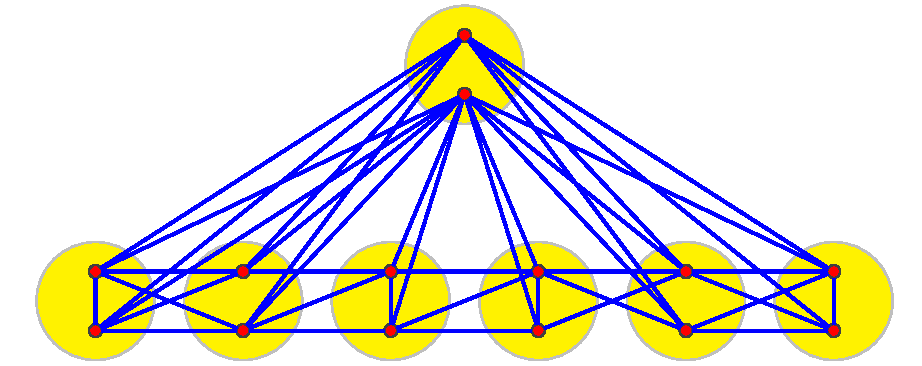
\includegraphics{figs/FanPartition}
    \caption{A 2-blowup of a fan.}
    \label{2blowup}
\end{figure}

%\david{Move restatement of \cref{main_thm_planar} bandwidth  here? One issue is that the discussion about bandwidth below depends on path-partition-width, which is not yet introduced. One could describe the restatement of \cref{main_thm_planar} without mentioning path-partitions, but it would be unatural. Another alternative is to also move the paragraph about $H$-partitions to here, but then the prevous results section gets delayed. Any thoughts? I am leaning towards moving the stuff on $H$-partitions and the stuff on bandwidth here, and call it `Equivalent Formulations'. Any thoughts?}

%\gwen{We discussed it with Piotr: What about keeping it as short as possible here: just defining bandwidth and stating the equivalent statement of thm 1 in terms of bandwidth, and that's it?}

%\pat{I agree with the second option. Define bandwidth and give the equivalent statement of \cref{main_thm_planar} for bandwidth.  In the section on $\mathcal{H}$-partitions we can explain the relationship between bandwidth and path partitions.}

\cref{main_thm_planar} can be restated in terms of the following classical graph parameter. The \defin{bandwidth} of a graph $G$ is the minimum integer $k$ such that there is an ordering $v_1,\dots,v_n$ of $V(G)$ such that $|i-j|\leq k$ for each edge $v_iv_j\in E(G)$. See \citep{CS89,ST20,ABET20,BPTW10,rao:small,BST09,feige:approximating} for a handful of important references on this topic. As explained in \cref{Bandwidth} below, \cref{main_thm_planar} is equivalent to the following:

\begin{thm}\label{main_thm_planar_restated}
  Every $n$-vertex planar graph $G$ has a set $X$ of $O(\sqrt{n}\log^2 n)$ vertices such that $G-X$ has bandwidth $O(\sqrt{n}\log^2 n)$.
\end{thm}

We in fact prove several generalizations of \cref{main_thm_planar_restated} that (a) study the tradeoff between $|X|$ and the bandwidth of $G-X$, and (b) consider more general graph classes than planar graphs.


\subsection{Previous Results}

As summarized in \cref{results_table}, we now compare \cref{main_thm_planar} with results from the literature, starting with the celebrated \defin{Planar Separator Theorem} due to \citet{lipton.tarjan:separator}, which states that any $n$-vertex planar graph $G$ contains a set $X$ of $O(\sqrt{n})$ vertices such that each component of $G-X$ has at most $n/2$ vertices. This theorem quickly leads to results about the blowup structure of planar graphs.  By applying it recursively, it shows that any $n$-vertex planar graph $G$ is contained in a graph that can be obtained from the closure of a %binary
tree of height $O(\log n)$ by blowing up the nodes of depth $i$ into cliques of size $O(\sqrt{n/2^i})$
%\david{To get a binary tree we need to group the components (after deleting the separator) into two groups, each of size at most $\frac23n$. So should $O(\sqrt{n/2^i})$ be $O(\sqrt{n/(\frac32)^i})$. Or we keep $O(\sqrt{n/2^i})$ and drop `binary'}.  \pat{Let's drop `binary'}
By applying it differently, \citet{lipton.tarjan:applications} show that $G$ is contained in a graph obtained from a star by blowing up the root into a clique of size $n^{1-a}$ and blowing up each leaf into a clique of size $O(n^{2a})$. These two structural results have had an enormous number of applications for algorithms, data structures, and combinatorial results on planar graphs. The second result, with $a=n^{1/3}$, shows that $G$ is contained in an $O(n^{2/3})$-blowup of a star. \citet{DvoWoo} use the Planar Separator Theorem to show that $G$ is contained in the $O(\sqrt{n})$-blowup of the closure of a tree %(not necessarily binary)
of height $O(\log\log n)$. That is, $G$ is contained in the $O(\sqrt{n})$-blowup of a graph of treedepth $O(\log\log n)$.

\begin{table}[!ht]
\centering
\caption{
%\piotr{I worked a bit on this table. I hope you like it more :P}\pat{Very nice, thanks!}
%\piotr{How about switching the order of columns? Lower bounds left and upper bounds right?} \pat{Sure.}
Previous and new results on $k$-blowups of a graph $H$ that contain every $n$-vertex graph $G$ from graph class $\mathcal{G}$.}
\begin{tabular}{llclcl}
\toprule
class $\mathcal{G}$ &$H$
&\multicolumn{2}{c}{lower bound on $k$}
&\multicolumn{2}{c}{upper bound on $k$}\\
  \midrule
\multirow{5}{*}{planar} & tree &
 $\Omega(n^{2/3})$ & \cite{LMST08}
 & $O(n^{2/3})$& \cite{lipton.tarjan:applications}\\[1.5ex]
& $\tw\leq2$
& $\Omega(\sqrt{n})$ &
& $O(\sqrt{n})$ & \cite{distel.dujmovic.ea:product}\\[1.5ex]
& fan
& $\Omega(\sqrt{n})$ &
& $O(\sqrt{n}\log^2 n)$ & \cref{main_thm_planar}\\[1.5ex]
& $\tw\leq3$
& $\Omega(\tw(G))$ &
& $\tw(G)+1$ &  \cite{ISW}\\[1.5ex]
& $\td\leq c$
& $\Omega(n^{1/2+\epsilon})$ & \cite{DvoWoo}
& $O(n^{1/2+\epsilon})$ & \cite{DvoWoo}\\[1ex]
\midrule
   planar $\mathrm{deg}\le \Delta$ & tree
   & $\Omega(\mathcolor{red}{\Delta^{1/3}}\cdot\tw(G))$ & \cite{LMST08}
   & $O(\Delta\cdot\tw(G))$ & \cite{ding.oporowski:some}\\
\midrule
     maximum degree $\Delta$  & tree
     & $\Omega(\Delta\cdot\tw(G))$ & \color{red}{\cite{Wood09}}
     & $O(\Delta\cdot\tw(G))$ & \cite{ding.oporowski:some,Wood09}\\
\midrule
    $K_t$-minor-free & $\tw\leq t-2$
    & $\Omega(\sqrt{n})\mathcolor{red}{(?!)}$ &
    & $O(\sqrt{tn})$ & \cite{ISW}\\[1.5ex]
    $K_t$-minor-free & $\tw\leq t-2$
    & $\mathcolor{red}{(?!)}$ &
    & $\tw(G)+1$ & \cite{ISW}\\[1.5ex]
    $K_t$-minor-free & $\tw\leq4$
    & $\Omega(t\sqrt{n})$ &
    & $O_t(\sqrt{n})$ & \cite{distel.dujmovic.ea:product}\\[1.5ex]
    $K_{3,t}$-minor-free & $\tw\leq 2$
    &&& $O(t\sqrt{n})$ & \cite{distel.dujmovic.ea:product}\\
\midrule
     & fan
     & $\Omega(\sqrt{gn})$ & \cite{DEW17}
     & $O(\sqrt{gn}+\sqrt{n}\log^2 n)$ & \cref{main_thm_genus}\\[1.5ex]
    genus-$g$ & $\tw\leq 2$
    &  &
    & $O((g+1)\sqrt{n})$& \cite{distel.dujmovic.ea:product}\\[1.5ex]
     & $\tw\leq3$
     &  &
     & $2(g+1)(\tw(G)+1)$ & \cite{ISW}\\
\midrule
    $k$-planar & fan
    & $\Omega(\sqrt{kn})$ & \cite{DEW17}
    & $O(k^{5/4}\sqrt{n}\log^2 n)$ & \cref{main_thm_k_planar}\\
\midrule
    apex-minor-free & fan
    & $\Omega(\sqrt{n})$ &
    & $O(\sqrt{n}\log^2 n)$ & \cref{main_thm_apexmf}\\
\midrule
    $Q\boxtimes P$ subgraph & fan
    & %$\Omega(\sqrt{\tw(Q)\cdot n})$
    &
    & $O(\sqrt{\tw(Q)\,n}\log^2 n)$ & \cref{main_thm_products}\\
    \bottomrule
\end{tabular}
\label{results_table}
\end{table}

\david{delete ``Previous and new'' from the caption?}

\david{we never explain the $\Delta^{1/3}\cdot \tw(G))$ lower bound. So I would remove this line from the table. }

\david{There are genus $g$ graphs with treewidth $\Omega(\sqrt{gn}$, so we can add $\Omega(\sqrt{gn}$ as a lower bound for genus $g$ graphs. For the same reason, there are $K_{3,t}$-minor-free graphs with treewidth $\Omega(\sqrt{tn}$. So we can add $\Omega(\sqrt{tn}$ as a lower bound for $K_{3,t}$-minor-free graphs. Similarly, we can add $\Omega(\sqrt{\tw(Q)\,n})$ as  a lower bound in the last line.}

\david{the red characters can be removed}

%\david{Where does the lower bound $\Omega(\sqrt{\tw(Q)\cdot n})$ come from?} \pat{I can't remember.} \david{let's remove it} \pat{Agreed}

Using different methods, \citet{ISW} show that every $n$-vertex planar graph is contained in a $O(\sqrt{n})$-blowup of a graph with treewidth 3. Thus, in the above question, one can take $\mathcal{H}$ to be the class of treewidth-$3$ graphs.\footnote{A \defin{tree-decomposition} of a graph $G$ is a collection $(B_x)_{x \in V(T)}$ of subsets of $V(G)$ indexed by a tree $T$, such that: (a) for every edge ${vw \in E(G)}$, there exists a node ${x \in V(T)}$ with ${v,w \in B_x}$, and (b) for every vertex ${v \in V(G)}$, the set $\{ x \in V(T) \colon v \in B_x \}$ induces a non-empty (connected) subtree of $T$. The \defin{width} of such a tree-decomposition is ${\max\{ |B_x| \colon x \in V(T) \}-1}$. A \defin{path-decomposition} is a tree-decomposition where the underlying tree is a path, denoted by the corresponding sequence of bags. The \defin{treewidth $\tw(G)$} of a graph $G$ is the minimum width of a tree-decomposition of $G$. The \defin{pathwidth $\pw(G)$} of a graph $G$ is the minimum width of a path-decomposition of $G$. Treewidth is the standard measure of how similar a graph is to a tree. Pathwidth is the standard measure of how similar a graph is to a path. By definition, $\tw(G)\leq\pw(G)$ for every graph $G$.}
Improving this result, \citet{distel.dujmovic.ea:product} show that even the class of treewidth-$2$ graphs is sufficient. They  ask whether every planar graph is contained in an $O(\sqrt{n})$-blowup of a bounded pathwidth graph.
Since fans have pathwidth $2$, \cref{main_thm_planar} answers this question, with $O(\sqrt{n})$ replaced by $O(\sqrt{n}\log^2 n)$.  With the exception of the star result (which requires an $\Omega(n^{2/3})$ blowup), all these results require blowing up a graph with many high-degree vertices.  \Cref{main_thm_planar} shows that a pathwidth-$2$ graph with one high-degree vertex is enough, with a quasi-optimal blowup of $O(\sqrt{n}\log^2 n)$.  Thus, \cref{main_thm_planar} offers a significantly simpler structural description of planar graphs than previous results.



\david{perhaps all the entries in the table where the upper bound is $O(\tw(G))$ should be presented and discussed separately. They are qualitatively different from $O(\sqrt{n})$ bounds.}
\gwen{What about removing them? That material is less relevant.} \david{It is less relevant, but still relevant. if we omitted it, then a referee could easily say we are ignoring parts of the literature that are in one sense stronger than our results (in the blowup size). I have added the next paragraph. Is it okay? Feel free to suggest revisions.}

% (We remark that the previous results \cite{ISW,distel.dujmovic.ea:product} have no polylogarithmic factors.  Every planar graphs is contained in a $O(\sqrt{n})$-blowup of a treewidth-$2$ graph \cite{distel.dujmovic.ea:product}.)

We now review results in the literature that show that every planar graph $G$ is contained in the blowup of a bounded treewidth graph, where the blowup factor is a function of the treewidth of $G$. This direction was introduced by \citet{UTW}, who defined the \defin{underlying treewidth} of a graph class $\GG$ to be the minimum integer $k$ such that for some function $f$ every graph $G\in\GG$ is contained in a $f(\tw(G))$-blowup of a graph $H$ with $\tw(H)\leq k$. \citet{UTW} showed that the underlying treewidth of the class of planar graphs equals 3. In particular, every planar graph $G$ with $\tw(G)\leq t$ is contained in a $O(t^2\log t)$-blowup of a graph with treewidth 3. \citet{ISW} improved this blowup factor to $t+1$, which is $O(\sqrt{n})$ (since planar graphs have treewidth $O(\sqrt{n})$) and might be significantly less than $O(\sqrt{n})$.  However, in this setting, treewidth 3 is best possible. In particular, \citet{UTW} showed that for any function $f$, there are planar graphs $G$ such that if $G$ is contained in a $f(\tw(G))$-blowup of a graph $H$, then $H$ contains $K_4$ and thus has treewidth at least 3. Allowing blowups of size $O(\sqrt{n})$ enables substantially simpler graphs $H$. \citet{distel.dujmovic.ea:product} showed that $\tw(H)\leq 2$ suffices. Allowing for an extra $O(\log^2n)$ factor in the blowup, this paper goes further and shows that a fan $H$ suffices, which has pathwidth 2. Note that for $K_t$-minor-free graphs (which also have treewidth $O_t(\sqrt{n})$~\citep{AST90}), there is a similar distinction between $f(\tw(G))$-blowups and $O_t(\sqrt{n})$-blowups. \citet{UTW} showed that the underlying treewidth of the class of $K_t$-minor-free graphs equals $t-2$, whereas 
\citet{distel.dujmovic.ea:product} showed that $\tw(H)\leq 4$ suffices for $O_t(\sqrt{n})$-blowups of $H$. See \citep{DHHJLMMRW} for more results on underlying treewidth. 

%\pat{The LMST graph is planar, has treewidth $\tw(G)\le O(k)$, maximum degree $\Delta\in O(k^3)$, and requires bags of size $\Omega(k^2)=\Omega(\Delta^{1/3}\tw(G))$.  We can improve this to $\Delta^{2/5}$, but the proof is a bit too long to put here.}

% Line 6: Where does the $\sqrt{t}$ in the lower bound come from? \pat{I thought $t^{3/2}\sqrt{n}$ was tight for the treewidth of $K_t$-minor free graphs, but apparently not.  Is that really not known?} \david{The tight bound is $\Theta(t \sqrt{n})$. The aupper bound was proved by Reed--Kawabarayashi. The lower bound holds since $\Omega(\sqrt{gn})$ is a lower bound for genus $g$ graphs.}\\
% Line 7: Where does the $t^{3/2}$ in the lower bound come from? There is a lower bound of $\Omega(t\sqrt{n})$ here.\pat{Same reason.} \\
% Line 8: There is a lower bound of $\Omega(\sqrt{gn})$ here, since there exists $n$-vertex graphs with genus $g$ and $\tw(G)\in \Omega(\sqrt{gn})$. This also explains the $\Omega(t\sqrt{n})$ lower bound in line 7.\\
% Line 9: cite \citet{DEW17} for the lower bound; we proved there are $(g,k)$-planar graphs with $\tw(G)\in\Omega(\sqrt{(g+1)(k+1)n})$.\\
% Line 11: $H$ is used to refer to two different graphs

% \noindent
% \framebox{\begin{minipage}{\textwidth}
% \pat{The LMST graph has treewidth $\tw(G)\le O(k)$, maximum degree $\Delta(G)\in O(k^3)$, and requires bags of size $\Omega(k^2)=\Omega(\Delta^{1/3}\tw(G))$. We can improve this a bit using the following modification of the LMST graph:  First remove all the edges incident to $r$.  Replace these with a set of $z:=2k^{5/3}$ stars where each star has a root $c_i$ that is adjacent to $r$ and to $k^3/z=k^{4/3}/2$ consecutive vertices of $P$.  The maximum degree in the resulting graph is achieved by $r$, which has degree $\Delta:=z \in O(k^{5/3})$. Call the vertices $c_1,\ldots,c_z$ \defin{centers}.  If we pick our parameters carefully, then each center is adjacent to the vertices of $k^{1/3}/2$ different ribs and each rib is adjacent to exactly one center, which we call the \defin{center} of the rib. \\[2ex]
% Let $\{V_x:x\in V(T)\}$ be a tree partition of $G$. Define the bag $V_a\supseteq \{r\}$ and the component $S$ of $G[V_a]$ that contains $r$ as before.  Say that $V_a$ avoids a rib if $V_a$ does not contain a vertex of the rib or the center of the rib.  Since $|V_a|\le w$, there are at least $z-w$ centers $c_i$ such that $V_a$ avoids all the ribs centered at $c_i$. Let $I$ index this set of centers and let $J$ index the set of ribs with centers indexed by $I$.  Then $|I|\ge z-w$ and $|J|\ge (z-w)k^{1/3}/2$.\\[2ex]
% Since some row of $G$ contains less than $w/k$ vertices of $V_a$, $G-V_a$ has at most $w/k$ components.  Therefore, there is a set $J'\subseteq J$ of ribs of size at least $k|J|/w$ such that all the ribs indexed by $J'$ are in a single component of $G-V_a$.  Therefore $T$ contains an edge $ab$ such that $V_b$ contains the center of every rib indexed by $J'$.  Now some component of $G-V_a-V_b$ contains at least $k|J'|/w$ of the ribs indexed by $J'$.  Let $J''\subseteq J'$ index this set. The top of each rib indexed by $J''$ has $k$ vertices that are all adjacent to a center in $V_b$.  Therefore $T$ contains an edge $bc$ such that $|V_c|\ge k|J''|$.  For $w \le k^{5/3}$, we get
% \[
%   w \ge |V_c|\ge k|J''| \ge \frac{k^2|J'|}{w} \ge \frac{k^3|J|}{w^2} \ge \frac{(z-w)k^{10/3}}{2w^2} = \frac{(2k^{5/3}-w)k^{10/3}}{2w^2} \ge \frac{(k^{5/3})k^{10/3}}{10w^2}
%   = \frac{k^{5}}{2w^2} \enspace .
% \]
% Rewriting this gives $w\ge k^{5/3}/\sqrt[3]{2}$.\\[2ex]
% Now $\tw(G)\le k$, so $w\in \Omega(k^{2/3}\tw(G))\ge \Omega(\Delta^{2/5}\tw(G))$.
% }
% \end{minipage}}

\subsection{Optimality}

We now explain why, except possibly for the $\log^2 n$ factor, \cref{main_thm_planar} cannot be strengthened.

\david{perhaps this paragraph should go in the opening subsection, what do you think?} The $\sqrt{n}$ factor in the size of the blowups used in these results is not arbitrary. A $k$-blowup of a treewidth-$t$ graph $H$ has treewidth at most $k(t+1)-1$.  Since there are $n$-vertex planar graphs of treewidth $\Omega(\sqrt{n})$ (such as the $\sqrt{n}\times\sqrt{n}$ grid), any result like \cref{main_thm_planar} that finds all planar graphs in blowups of bounded treewidth graphs must have blowups of size $\Omega(\sqrt{n})$.

% Note that a graph of treewidth $k(t+1)-1$ has a balanced separator of size $k(t+1)$. Thus, the results of \cite{ISW,distel.dujmovic.ea:product} imply and strengthen the Lipton-Tarjan Planar Separator Theorem \cite{lipton.tarjan:separator}


% \david{I suggest we argue that the question in the opening paragraph is motivated by the desire for qualitative strengthenings of the Lipton-Tarjan Planar Separator Theorem (allowing a $\polylog n$ factor) that describe the global structure of planar graphs.}
% \pat{Ok, how about we open with a statement of the Lipton-Tarjan theorem. The Lipton-Tarjan Theorem has several implications about the global structure of any planar graph $G$.  By applying it recursively, it shows that any planar graph $G$ is contained in a graph that can be obtained from the closure of a binary tree of height $O(\log n)$ by blowing up the nodes of depth $i$ into cliques of size $O(\sqrt{n/2^i})$.  By applying it differently, Lipton and Tarjan show that $G$ is contained in a graph obtained from a star by blowing up the root into a clique of size $n^{1-a}$ and blowing up each leaf into a clique of size $n^{2a}$.  These two results have had an enormous number of applications for algorithms, data structures, and combinatorial results on planar graphs.  The second result, with $a=n^{1/3}$ shows that $G$ is contained in an $O(n^{2/3})$-blowup of a star. Dvorak and Wood use the Lipton-Tarjan theorem to show that $G$ is contained in the $O(\sqrt{n})$-blowup of the closure of a tree (not binary) of height $O(\log\log n)$. That is, $G$ is contained in the $O(\sqrt{n})$-blowup of a graph of treedepth $O(\log\log n)$.  Using other techniques, Distel et al show that $G$ is contained in a $O(\sqrt{n})$-blowup of a treewidth-$2$ graph.  With the exception of the star result (which requires an $\Omega(n^{2/3})$ blowup), all of these require blowing up a graph with many high-degree vertices.  We show that a pathwidth-$2$ graph with one high-degree vertex is enough, with a quasi-optimal blowup of $O(\sqrt{n}\log^2 n)$.} \david{This is great material. However, I like how the current intro gets to our main result very quickly. Does it work to add this discussion after our opening theorem statement?}


Pathwidth $2$ is also the best possible bound in results like  \cref{main_thm_planar}.  Indeed, even \emph{treewidth} $1$ is not achievable:  \citet{LMST08} describe an infinite family of $n$-vertex planar graphs $G$ such that every (improper) 2-colouring has a monochromatic component on $\Omega(n^{2/3})$ vertices. Say $G$ is contained in a $k$-blowup $(K_v:v\in V(T))$ of a tree $T$. Colour each vertex in each $K_v$ by the colour of $v$ in a proper 2-colouring of $T$. So each monochromatic component is contained in some $K_v$, implying that $k\in\Omega(n^{2/3})$.
% The bound $O(n^{2/3})$ is achievable: Every $n$-vertex planar graph $G$ has a set $X$ of $O(n^{2/3})$ vertices such that every component of $G-X$ has size $O(n^{2/3})$ \cite{lipton.tarjan:applications}.  This implies that $G$ is an $O(n^{2/3})$-blowup of a star, where the set $X$ maps to the root of the star and each component of $G-X$ maps to a different leaf of the star.

% The lower-bound construction of \citet{LMST08} contains a vertex of very high degree, and this is necessary.  A classic result of \citet{ding.oporowski:some} implies that if $G$ is planar and has maximum degree $\Delta$ then $G$ is contained in the $O(\Delta\sqrt{n})$-blowup of a tree.

Any graph of treedepth $c$ has pathwidth at most $c-1$, so it is natural to ask if \cref{main_thm_planar} can be strengthened to show that every $n$-vertex planar graph is contained in a $\tilde{O}(\sqrt{n})$-blowup of a bounded treedepth graph.  The answer is no, as we now explain. \citet[Theorem~19]{DvoWoo} show that, for any $c\geq 1$ there exists $\epsilon>0$ such that if the $\sqrt{n}\times\sqrt{n}$ grid is contained in a $k$-blowup of a graph $H$ with treedepth at most $c$, then $k\geq\Omega(n^{1/2+\epsilon})$. Thus the $\sqrt{n}\times \sqrt{n}$-grid is not contained in a $\tilde{O}(n^{1/2})$-blowup of a graph with bounded treedepth.  In particular, \cref{main_thm_planar} cannot be strengthened to the treedepth setting without increasing the size of the blowup by a polynomial factor.

%\david{I don't understand this final sentence.} \pat{It said 'can' when it should have said 'cannot'}. \david{that makes more sense}

%  are contained
% A graph of treedepth at most
% The class of bounded treedepth graphs is more re
%
%
%
%
%
% Results of \citet[Theorem~5]{DvoWoo} imply that for all $\epsilon>0$ there exists $c$ such that every $n$-vertex planar graph is contained in a $O(n^{1/2+\epsilon})$-blowup of a graph $H$ with treedepth $c$, which is a  stronger property than bounded pathwidth, and indeed implies $\pw(H)\leq c-1$. \citet[Theorem~19]{DvoWoo} also establish a corresponding lower bound: for any $c\geq 1$ there exists $\epsilon>0$ such that if the $\sqrt{n}\times\sqrt{n}$ grid is contained in a $k$-blowup of a graph $H$ with treedepth at most $c$, then $k\geq\Omega(n^{1/2+\epsilon})$. (In fact, these lower and upper bounds match.)\ Thus the $\sqrt{n}\times \sqrt{n}$-grid is not contained in a $\tilde{O}(n^{1/2})$-blowup of a graph with bounded treedepth. In this sense, the `bounded pathwidth' condition in \cref{main_thm_planar} is best posible.


% \david{Stuff to add to the intro:
% \begin{itemize}
% % \item $O(\sqrt{n})$ blowups of bounded treewidth graphs imply and strengthen the Lipton--Tarjan separator theorem. Without this, the naive reader will ask ``what is the point?''
% % \item \citet{distel.dujmovic.ea:product} asked whether every $n$-vertex planar graph is contained in a $O(\sqrt{n})$-blowup of a graph with bounded pathwidth. \cref{main_thm_planar} shows the answer is ``yes'' with $O(\sqrt{n})$ replaced by $\tilde{O}(\sqrt{n})$.
% \item Results of \citet[Theorem~5]{DvoWoo} imply that for all $\epsilon>0$ there exists $c$ such that every $n$-vertex planar graph is contained in a $O(n^{1/2+\epsilon})$-blowup of a graph $H$ with treedepth $c$, which is a  stronger property than bounded pathwidth, and indeed implies $\pw(H)\leq c-1$. \citet[Theorem~19]{DvoWoo} also establish a corresponding lower bound: for any $c\geq 1$ there exists $\epsilon>0$ such that if the $\sqrt{n}\times\sqrt{n}$ grid is contained in a $k$-blowup of a graph $H$ with treedepth at most $c$, then $k\geq\Omega(n^{1/2+\epsilon})$. (In fact, these lower and upper bounds match.)\ Thus the $\sqrt{n}\times \sqrt{n}$-grid is not contained in a $\tilde{O}(n^{1/2})$-blowup of a graph with bounded treedepth. In this sense, the `bounded pathwidth' condition in \cref{main_thm_planar} is best posible.
% \end{itemize}}


\subsection{Graphs on Surfaces and With Crossings}

\cref{main_thm_planar} generalizes for graphs embeddable on arbitrary surfaces as follows. Here, the \defin{Euler genus} of a surface obtained from a sphere by adding $h$ handles and $c$ crosscaps is $2h+c$. The \defin{Euler genus} of a graph $G$ is the minimum Euler genus of a surface in which $G$ embeds without crossings.

\begin{thm}\label{main_thm_genus}
  Every $n$-vertex graph with Euler genus $g$ is contained in a $O(\sqrt{gn}+\sqrt{n}\log^2 n)$-blowup of a fan.
\end{thm}

\cref{main_thm_planar} also generalizes for graphs that can be drawn with a bounded number of crossings on each edge. A graph $G$ is \defin{$k$-planar} if it has a drawing in the plane in which each edge is in at most $k$ crossings. This topic is important in the graph drawing literature; see \cite{KLM17} for a survey just on the $k=1$ case. We prove the following generalization of \cref{main_thm_planar}:

\begin{thm}\label{main_thm_k_planar}
  Every $n$-vertex $k$-planar graph is contained in a $O(k^{5/4}\sqrt{n}\log^2 n)$-blowup of a fan.
\end{thm}

We in fact prove the following generalization of \cref{main_thm_planar,main_thm_k_planar}. Here a graph $G$ is \defin{$(g,k)$-planar} if it has a drawing in a surface of Euler genus at most $g$ in which each edge is in at most $k$ crossings.

\begin{thm}
\label{main_thm_gk_planar}
%For any integers $g,k\geq 0$, every $n$-vertex $(g,k)$-planar graph $G$ has a set $X$ of $O((k+1)^{3/4}(g+1)^{3/4}n^{1/2} + (k+1)^{5/4} n^{1/2} \log^2 n)$ vertices such that $G-X$ has bandwidth at most $O((g+1)^{1/2}(k+1)^{5/4}n^{1/2}\log^2 n)$.
Every $n$-vertex $(g,k)$-planar graph is a $O( (k+1)^{5/4}n^{1/2}(\log^2 n) \, \max\{ (g+1)^{1/2},(g+1)^{3/4}(k+1)^{-1/2} \log^{-2} n\} )$-blowup of a fan.
\end{thm}

% \david{The max here is annoying, but I don't see how to eliminate it, since it is possible that $(g+1)^{1/4} \geq (k+1)^{1/2}\log^2n$.}


Note that if $n\gg g$ then the upper bound in
\cref{main_thm_gk_planar} simplifies to  $O( (g+1)^{1/2}(k+1)^{5/4}n^{1/2}\log^2 n )$, which matches the bound in \cref{main_thm_genus}. In particular, \cref{main_thm_gk_planar} with $g=0$ implies \cref{main_thm_k_planar}.  The proofs of \cref{main_thm_genus,main_thm_k_planar,main_thm_gk_planar} are presented in \cref{genus_section}.

%\david{Scrap \cref{main_thm_k_planar}? It is implied by \cref{main_thm_gk_planar} with $g=0$.} \gwen{I'd prefer to keep a separate statement for $k$-planar graphs, Thm 4 is not easy to read} \david{okay}

% \cref{main_thm_genus,main_thm_k_planar} can be combined.  A graph is \defin{$(g,k)$-planar} if it has a drawing on a surface of Euler genus $g$ in which each edge crosses at most $k$ other edges.
%
% \begin{thm}\label{main_thm_gk_planar}
%   Every $n$-vertex $(g,k)$-planar graph is contained in a $O(\sqrt{gn}+k^{5/4}\sqrt{n}\log^2 n)$-blowup of a fan.
% \end{thm}



\subsection{Apex-Minor-Free Graphs}

\cref{main_thm_planar,main_thm_genus} generalize for other minor-closed classes as follows. A graph $X$ is a \defin{minor} of a graph $G$ if a graph isomorphic to $X$ can be obtained from a subgraph of $G$ by edge contractions. A graph $G$ is \defin{$X$-minor-free} if $X$ is not a minor of $G$. A graph $X$ is \defin{apex} if $X-a$ is planar for some vertex $a\in V(X)$. For example, $K_5$ is apex and planar graphs are $K_5$-minor-free. More generally, the complete bipartite graph $K_{3,2g+3}$ is apex and it follows from Euler's formula that graphs with Euler genus $g$ are $K_{3,2g+3}$-minor-free. Thus, apex-minor-free graphs are a broad generalization of planar graphs and graphs of bounded Euler genus that have received considerable attention in the literature~\citep{demaine.hajiaghayi.ea:approximation,dragan.fomin.ea:ptas,fomin.lokshtanov.ea:subexponetial,dvorak.thomas:list,korhonen.nadara.ea:fully}.

 % \citet{dujmovic.joret.ea:planar} showed that for every apex graph $X$ there exists $c$ such that every $X$-minor-free graph has row treewidth at most $c$ (and such a theorem holds only if $X$ is apex). \cref{main_thm_products} thus implies:

\begin{thm}\label{main_thm_apexmf}
For every fixed apex graph $X$, every $n$-vertex $X$-minor-free graph is contained in a $O(\sqrt{n}\log^2 n)$-blowup of a fan.
\end{thm}

%\david{I think we need to `sell' \cref{main_thm_apexmf} more, especially since a large part of the paper is dedicated to its proof.} \pat{I agree, but I have to no idea what to say about apex minor free graphs.} \david{One option is to put Section 1.4 first, then put the corollaries for genus $g$, $k$-planar, $(g,k)$-planar, apex-minor-free graphs. This highlights the power of the $H\boxtimes P$ structure. And then afterwards say that we can get better bounds for genus $g$, $k$-planar, $(g,k)$-planar graphs using some ad-hoc arguments. This ordering puts the emphasis on the $H\boxtimes P$ structure. What do you think?  } \pat{I think I prefer the order of the introduction to match the order of presentation in the paper, which is what we currently have.  I also don't want to be seen as overselling the product structure result when you can get better results (much more easily) without it.  I'm happy with the current statement about them being a broad generalization of planar graphs that has been studied before. I've added references to some papers published in prestigious venues that focus specifically on apex-minor-free graphs.}

\subsection{Product Structured Graphs}

\Cref{main_thm_planar,main_thm_apexmf} each follow from a more general theorem about subgraphs of certain strong graph products, as we now explain.  The \defin{strong product} $A\boxtimes B$ of two graphs $A$ and $B$ is the graph with vertex set $V(A\boxtimes B):=V(A)\times V(B)$ that contains an edge with endpoints $(v_1,v_2)$  and $(w_1,w_2)$ if and only if
\begin{compactenum}
    \item $v_1w_1\in E(A)$ and $v_2=w_2$;
    \item $v_1=w_1$ and $v_2w_2\in E(B)$; or
    \item $v_1w_1\in E(A)$ and $v_2w_2\in E(B)$.
\end{compactenum}
Note that the $k$-blowup of $H$ can be written as the strong product $H\boxtimes K_k$.  Therefore, \cref{main_thm_planar} states that for every $n$-vertex planar graph $G$ there is a fan $F$ such that $G$ is isomorphic to a subgraph of $F\boxtimes K_{O(\sqrt{n}\log^2 n)}$.

%\david{We never use the $\rtw$ notation}

The \defin{row treewidth} of a graph $G$
%, denoted by $\rtw(G)$, 
is the minimum integer $t$ such that $G$ is contained in $H\boxtimes P$ for some graph $H$ with treewidth $t$ and for some path $P$. We prove the following more general result:

% Then \cref{main_thm_products} becomes: \\
% Every $n$-vertex graph with row-treewidth $t$ is contained in a $O(t\sqrt{n}\log^2 n)$-blowup of a fan.\\
% Much of the following discussion would be simplied.
% }

\begin{thm}\label{main_thm_products}
  Every $n$-vertex graph with row treewidth $t$ is contained in a $O(\sqrt{tn}\log^2 n)$-blowup of a fan.
\end{thm}

Although we give a more direct proof of \cref{main_thm_planar}, \cref{main_thm_products} implies \cref{main_thm_planar} by the following \defin{Planar Graph Product Structure Theorem}:

\begin{thm}[\cite{dujmovic.joret.ea:planar,ueckerdt.wood.ea:improved}]\label{planar_product_structure}
  Every planar graph has row treewidth at most $6$.
\end{thm}

\Cref{main_thm_products} implies \cref{main_thm_apexmf} by the following \defin{Apex-Minor-Free Graph Product Structure Theorem}:

\begin{thm}[\cite{dujmovic.joret.ea:planar}]\label{apexmf_product_structure}
  For every apex graph $X$ there exists $c$ such that every $X$-minor-free graph has row treewidth at most $c$.
\end{thm}

Variants of \cref{main_thm_genus,main_thm_k_planar,main_thm_gk_planar} also follow from \cref{main_thm_products} and product structure theorems for genus-$g$ graphs, $k$-planar graphs and $(g,k)$-planar graphs~\cite{dujmovic.joret.ea:planar,distel.hickingbotham.ea:improved,dujmovic.morin.ea:graph,distel.hickingbotham.ea:powers}, but this produces results with a larger dependence on $g$ or $k$.

% \david{delete the following paragraph?} \Cref{planar_product_structure} has been generalized to a number of other minor-closed and non-minor closed graph classes (with $6$ replaced by some value that depends on the graph class), including bounded genus graphs and (more generally) apex-minor-free graphs \cite{dujmovic.joret.ea:planar,distel.hickingbotham.ea:improved} and $k$-planar graphs \cite{dujmovic.morin.ea:graph,distel.hickingbotham.ea:powers}.

% \cref{main_thm_planar} generalises for graphs embeddable on arbitrary surfaces\footnote{The \defin{Euler genus} of a surface obtained from a sphere by adding $h$ handles and $c$ crosscaps is $2h+c$. The \defin{Euler genus} of a graph $G$ is the minimum Euler genus of a surface in which $G$ embeds without crossings.}.
% Building on previous work in \citep{dujmovic.joret.ea:planar,ueckerdt.wood.ea:improved}, \citet{distel.hickingbotham.ea:improved} show that every graph of Euler genus $g$ has row treewidth at most $2g+6$. \Cref{main_thm_products} thus implies:
%
% \begin{thm}\label{genus_products}
% Every $n$-vertex graph of Euler genus $g$ is contained in a $O((g+1)\sqrt{n}\log^2 n)$-blowup of a fan.
% \end{thm}
%
% \pat{\Cref{genus_products} can be improved without using graph products. Every $n$-vertex genus-$g$ graph $G$ has a set of $X_0$ of $O(\sqrt{gn})$ vertices such that $G-X_0$ is planar \cite{eppstein:dynamic}. Apply \cref{main_thm_planar} to $G-X_0$ to get $X'$ of size $O(\sqrt{n}\log^2 n)$ such that $G-X_0-X'$ has bandwidth $O(\sqrt{n}\log^2 n)$.  Now take $X:=X_0\cup X'$ to get a set $X$ of size $O(\sqrt{gn} + \sqrt{n}\log^2 n)$ such that $G-X$ has bandwidth $O(\sqrt{n}\log^2 n)$.}
%
% \david{Good point, pulling out $O(\sqrt{n})$ vertices is very powerful. }


% Product structure theorems are known for various non-minor-closed classes~\citep{dujmovic.morin.ea:graph,HW24,distel.hickingbotham.ea:powers}. For example, a graph is \defin{$(g,k)$-planar} if it has a drawing in a surface of Euler genus $g$ with at most $k$ crossings on each edge. \citet{dujmovic.morin.ea:graph} proved that every $(g,k)$-planar graph has row treewidth  $O((g+1)k^5)$. \Cref{main_thm_products} thus implies:
%
% \begin{thm}\label{gkplanar_products}
% Every $n$-vertex $(g,k)$-planar graph is contained in a $O((g+1)k^5\sqrt{n}\log^2 n)$-blowup of a fan.
% \end{thm}
%
% \pat{Here's a better result, again without using product structure:  By the crossing lemma, $G$ has $O(\sqrt{k} n)$ edges (for $g\in O(n)$).  Add a dummy vertex at each crossing in $G$ to get a genus-$g$ graph $G'$ with $O(k^{3/2}(n+g))$ vertices.  Let $X_0'$ be a planarizing set of $G'$ of size $O(\sqrt{k^{3/2}(n+g)g})=O(k^{3/4}(\sqrt{n}+g))$ (again, using \citet{eppstein:dynamic}). Replace every dummy $x$ in $X_0'$ with (at most four) real vertices corresponding to the two edges that cross at $x$.  Now $G-X_0'$ is $k$-planar.  Add a dummy vertex at each crossing in $G-X_0'$ to get a planar graph $G''$ with $O(k^{3/2}n)$ vertices. Apply \cref{planar_sparsifier} to $G''$ to get $X''$ of size $O((k^{3/2}n/D)\log n)$ such that $G''$ has local density $D$.  By \cref{rao}, $G''$ has bandwidth $O(D\log^3 n)$.  Replace each dummy vertex in $X''$ by the (at most $4$) corresponding real vertices and let $X:=X_0'\cup X''$.  Then $|X|=O(k^{3/2}(\sqrt{n}+g)+(k^{3/2}n/D)\log n)$.  Take the $O(D\log^3 n)$-bandwidth ordering of $G''-X''$ and use it for the vertices of $G-X$.  Each edge of $G-X$ corresponds to a path of length at most $k+1$ in $G''-X''$, so this ordering has bandwidth $O(kD\log^3 n)$.  Set $D:=k^{1/4}\sqrt{n}/\log n$ to conclude that $G$ has fan-partition-width $O(g\sqrt{k} + k^{5/4}\sqrt{n}\log^2 n)$.\\[2ex]
% It would be nice to shave off the ugly $k^{1/4}$ factor in this result.}
%
% \david{nice}

%\david{I think this generalises to $k$-gap-planar graphs. Here we have a drawing where each crossing is charged to one of the two edges, and each edge is charged with at most $k$ of its crossings. Basically, this says that every subgraph has an average number of crossings per edge of at most $k$, whereas $k$-planar requires a maximum number of crossings per edge of at most $k$. The same proof (using the crossing lemma) gives $|E(G)|\in O(\sqrt{k}n)$. For the extension to  surfaces, use Lemmas 4.5 and 4.6 in \citep{OOW19}.  UPDATE: the last part of Pat's argument fails, since there can be very long edges.}

% \david{
% Do we get improved depedennce working with subgraph of $H\boxtimes P \boxtimes K_c$? (e.g. for $k$-planar graphs we can use $\tw(H)=10^{10}$ and $c=c_k$).
% }

% \pat{Now I can answer the question: No, the bound will be $O(tc\sqrt{n}\log^2 n)$.  The bottleneck is the sparsification lemma.  The size of the set $X$ there becomes $O((t+1)c(n/D)\log n)$.  Interestingly (maybe) when $G$ is a subgraph of $H\boxtimes P\boxtimes K_c$, the metric space $(V(G),d_{H\boxtimes P\boxtimes K_c})$ has $(k,O(t\sqrt{\log n}))$-volume-respecting embeddings, for any $c$. If you take $t=0$ and $c=n$ then you get a metric space where $d(v,w)=1$ for all  $v,w\in V(G)$ and this has as $(k,O(\sqrt{\log n}))$-volume respecting embedding.  The proof of this is much simpler: Every vertex maps to a uniformly random point in a $O(k\log n)$-dimensional ball of diameter $1$ (so the radius of the ball is $O(1/\sqrt{k\log n}))$.  Then the proof ``just'' boils down to showing that, with probability at least $1-n^{-ck}$, $k$ random points in this ball define a $(k-1)$-simplex whose $(k-1)$-dimensional volume is $\Omega((1/((k-1)!\sqrt{\log n})^{k-1}))$. \\[2ex]
% We should somehow get this point across in the introduction:  The metric space $(V(G),d_G)$ is awkward to work with directly for the same reason that planar graphs are awkward to work with directly; it's hard to see any structure.  The metric space $(V(G),d_{K_n})$ is a contraction of $(V(G),d_G)$ which makes it suitable to work with, and it's highly regular, but it's too ``dense'' to have any useful properties.  The metric space $(V(G),d_{H\boxtimes P})$ is a perfect middle-ground; it's highly regular (like $(V(G),d_{K_n}))$ but ``sparse'' enough to admit a local sparsification lemma \david{include this paragraph as is}.\\[2ex]
% It might be a useful exercise to find what properties of a metric space are sufficient to prove a local sparsification lemma.  Here's a first try:\\[2ex]
% Let $(S,d)$ be a finite metric space, let $L_0\subseteq S$, and for each $0\le a\le b$, let $L_{[a,b]}:=\{x\in S: a\le d(x,L_0)\le b\}$.  Now I'm stuck.  There is no obvious notion of a set $X\subseteq S$ that separates two subsets $A,B$ of $S$.
% }

\subsection{Relation to $\mathcal{H}$-Partitions}
\label{bandwidth_relation}

For a graph $H$, an \defin{$H$-partition} of a graph $G$ is a partition $\mathcal{P}:=\{B_x: x\in V(H)\}$ of $V(G)$ whose parts are indexed by the vertices of $H$ such that, for each edge $vw$ of $G$, $v$ and $w$ are in the same part or there exists an edge $xy$ of $H$ such that $v\in B_x$ and $w\in B_y$.  The \defin{width} of $\mathcal{P}$ is the maximum size of any part.  It follows immediately from this definition that $G$ has an $H$-partition of width $w$ if and only if $G$ is contained in $H\boxtimes K_w$ if and only if $G$ is contained in a $w$-blowup of $H$. When $H$ is a member of some class $\mathcal{H}$ of graphs, we call an $H$-partition of $G$ an \defin{$\mathcal{H}$-partition} of $G$.  For example, if $H$ is path, tree, or fan, then we call an $H$-partition a path-partition, a tree-partition, or a fan-partition, respectively.  The \defin{$\mathcal{H}$-partition-width}  of a graph $G$ is the minimum integer $w$ such that $G$ has an $\mathcal{H}$-partition of width $w$. Thus, \cref{main_thm_planar} states that every $n$-vertex planar graph has fan-partition-width $O(\sqrt{n}\log^2 n)$.

%\david{Hyphenate $\mathcal{H}$-partition-width, fan-partition, fan-partition-width, path-partition, path-partition-width throughout}

\subsection{Relation to Bandwidth}
\label{Bandwidth}

Let $G$ be a graph and let $v_1,\ldots,v_n$ be an ordering of $V(G)$.
Then $v_1,\ldots,v_n$ has \defin{bandwidth} $\mathdefin{\bw_G(v_1,\ldots,v_n)}:=\max\{|j-i|: v_iv_j\in E(G)\}\cup\{0\}$.
The \defin{bandwidth} of $G$ is $\mathdefin{\bw(G)}:=\min\{\bw_G(v_1,\ldots,v_n):\text{$v_1,\ldots,v_n$ is an ordering of $V(G)$}\}$. The bandwidth of a graph $G$ is closely related to the path-partition-width of $G$.  Indeed, if $\bw_G(v_1,\ldots,v_n)=w$, and $P:=x_1,\ldots,x_{\lceil n/w\rceil}$ is a path, then setting $B_{x_i}:=\{v_j: (i-1)w+1 \le j \le iw\}$ for each $i\in\{1,\ldots,\lceil n/w\rceil\}$ gives a path-partition $\{B_{x}:x\in V(P)\}$ of width $w$.  In the other direction, if $P:=x_1,\ldots,x_k$ is a path and  $\{B_x:x\in V(P)\}$ is a path-partition of width $w$, then any ordering $v_1,\ldots,v_n$ of $V(G)$ that places all vertices of $B_{x_i}$ before those in $B_{x_{i+1}}$ for each $i\in\{1,\ldots,k-1\}$ has $\bw_G(v_1,\ldots,v_n)\le 2w-1$.

Thus, \cref{main_thm_planar} is equivalent to saying that every $n$-vertex planar graph $G$ has a set $X$ of  $O(\sqrt{n}\log^2 n)$ vertices (the part $B_{x_0}$ in a fan-partition of $G$) such that $G-X$ has bandwidth $O(\sqrt{n}\log^2 n)$ \david{The reader will have long ago forgotten what $x_0$ refers to, especially since it is buried in a footnote. Perhaps we should define `fan' in the main body of the start of the paper, without the $x_0,x_1,\dots,x_k$ notation. And give a name like `root part'  or `dominant part', which we can re-use here (and elsewhere?).}. We actually obtain the following slight strengthening of \cref{main_thm_planar}, since as shown above, if $\bw(G)\leq k$ then $G$ is contained in a $k$-blowup of a path on at most $\ceil{|V(G)|/k}$ vertices.

\begin{thm}\label{main_thm_planar_order}
  Every $n$-vertex planar graph is contained in a $O(\sqrt{n}\log^2 n)$-blowup of a fan with
  $O(\sqrt{n}/\log^2 n)$ vertices.
\end{thm}

The same improvement is applicable to \cref{main_thm_genus,main_thm_k_planar,main_thm_gk_planar,main_thm_apexmf}. 

% \pat{Note: \cref{main_thm_planar_order} gives an easy to understand graph with $O(n)$ vertices and $O(n^{3/2}\log^2 n)$ edges that contains every $n$-vertex planar graph as a subgraph, a result first shown (without the $\log^2 n$ factor) by \citet{babai.chung.ea:on}.  Probably not worth mentioning since much better results are known now.} \david{I agree to not mention this.}


\subsection{Techniques}

%\david{Should we say that all logs are base 2? it matters since we occasionally write $\log$ outside of a $O(...)$. Do we ever use non-base-2 logs?} \pat{We use $\ln n$ towards the end, since it's convenient for for amplifying probabilities.} \david{So I suggest we say that $\log$ means base 2 and $\ln$ means base $e$. Okay?} \pat{Okay}

Throughout the paper, we use $\log$ for the base-2 logarithm, and we use $\ln$ for the base-$e$ logarithm. 

For a graph $G$ and any two vertices $v,w\in V(G)$, define the \defin{(graph) distance} between $v$ and $w$, denoted $\mathdefin{d_G(v,w)}$, as the minimum number of edges in any path in $G$ with endpoints $v$ and $w$ or define $d_G(v,w):=\infty$ if $v$ and $w$ are in different components of $G$.  For any $r\ge 0$ and any $v\in V(G)$, let $\mathdefin{B_G(v,r)}:=\{w\in V(G):d_G(v,w)\le r\}$ denote the radius-$r$ ball in $G$ with center $v$.
The \defin{local density} of a graph $G$ is $\mathdefin{\ld(G)}:=\max\{(|B(v,r)|-1)/r:r> 0,\, v\in V(G)\}$.\footnote{The ${}-1$ in this definition of local density does not appear in the definitions of local density used in some other works \cite{feige:approximating,rao:small}, but this makes no difference to our asymptotics results.  Our definition makes for cleaner formulas and seems to be more natural. For example, under our definition, the local density of a cycle of length $2k+1$ is $2$ and every $r$-ball contains exactly $2r+1$ vertices for $r\in\{1,\ldots,k\}$. Without the ${}-1$, the local density of a cycle is $3$, but only because radius-$1$ balls contain three vertices.}

% } If $|B_G(v,r)|=Dr+1$ then in any permutation $v_1,\ldots,v_n$ of $V(G)$, one of the vertices $w$ in $B_G(v,r)\setminus \{v\}$ is at distance at least $Dr/2$ from $v$. That is, $v=v_i$ and $w=v_j$, and $|j-i|\ge Dr/2$.  Since $G$ contains a path with at most $r$ edges from $v$ to $w$, one of the edges $v_{i'}v_{j'}$ of this path must have $|i'-j'|\ge Dr/2r=D/2$.  Therefore $\bw(G)\ge\ld(G)/2$.


The local density of $G$ provides a lower bound on the bandwidth of $G$. For any ordering $v_1,\dots,v_n$ of $V(G)$ with bandwidth $b$, for each vertex $v_i$, $B_G(v_i,r) \subseteq \{v_{i-rb},\dots,v_{i+rb}\}$, so $|B_G(v_i,r)|\leq 2rb+1$ and $\ld(G)\leq 2\bw(G)$. \david{Let's add more to this story .... Erd\H{o}s~[ref?] conjectured that $\bw(G)\leq O(\ld(G))$ for every graph $G$. This was disproved by \citet{chvatalova:on} who described a family of $n$-vertex trees $T$ with local density at most $3$ and $\bw(T)\in\Omega(\log n)$. Thus, $\bw(G)$ is not upper bounded by any function of $\ld(G)$, even for trees. This remains true for trees of bounded pathwidth: \citet{CS89} describe a family of $n$-vertex trees $T$ with local density at most $9$, pathwidth $2$, and  $\bw(T)\in\Omega(\log n/\log\log n)$. On the other hand, in his seminal work, Fiege ...} 
On the other hand, $\bw(G)$ is not upper bounded by any function of $\ld(G)$. In fact, \citet{chvatalova:on} describes a family of $n$-vertex trees $T$ with local density at most $3$ and $\bw(T)\in\Omega(\log n)$.  \citet{CS89} even describe a family of $n$-vertex trees $T$ with local density at most $9$, pathwidth $2$, and  $\bw(T)\in\Omega(\log n/\log\log n)$.  In his seminal work, \citet{feige:approximating} proves that bandwidth is upper bounded by the local density times a polylogarithmic function of the number of vertices.

\pat{The correct reference is \citet{chvatalova:on}, who shows that a tree of local density $3$ having $c^k$ vertices has bandwidth $\Omega(k)$.  \citet{CS89} give a tree of pathwidth $2$ with $c^{k\log k}$ vertices and bandwidth $\Omega(k)$.} \david{So in the original sentence about \cite{CS89}, $\Omega(\log n)$ should be replaced by $\Omega(\log n/ \log\log n)$? \pat{Yes, done.} Anyway, 
\citet{chvatalova:on} predates \citep{CS89} by several years, so we should put the original reference. I would also mention \citet{CS89} since I think it is interesting there is an example with pathwidth 2. I think \citet{CCDG82} also has a construction.}. \pat{\citet{CCDG82} is fascinating.  Erd\"os conjectured that bandwidth was linear in local density, in my birth year. Chvátalová disproved it and also won a \$5 Erd\H{o}s prize for solving another question related to bandwidth.  I can't get my hands on her thesis, so we'll have to take Chung and Seymour's word for it.} \david{I have asked my library to get the  Chvátalová  thesis.}

\begin{thm}[\citet{feige:approximating}]
\label{feige_bandwidth_vs_density}
  For every $n$-vertex graph $G$,
  \[
    \bw(G)\in O\left(\ld(G)\cdot \log^3 n\sqrt{\log n\log\log n}\right) \enspace .
  \]
\end{thm}

\citet{rao:small} improves \cref{feige_bandwidth_vs_density} in the special case of planar graphs:%\footnote{\citet{rao:small} does not explicitly consider bandwidth, but his results on volume-preserving embeddings of planar graphs combined with the argument of \citet{feige:approximating} implies \cref{feige_bandwidth_vs_density}.}

\begin{thm}[\citet{rao:small}]
\label{rao_bandwidth_vs_density}
  For every $n$-vertex planar graph $G$,
  \[
    \bw(G)\in O\left(\ld(G)\cdot \log^3 n\right) \enspace .
  \]
\end{thm}

By \cref{rao_bandwidth_vs_density}, to prove \cref{main_thm_planar} it suffices to show the following \defin{local sparsification lemma}:

\begin{lem}\label{planar_sparsification_special}
  Every $n$-vertex planar graph $G$ has a set $X$ of $O(\sqrt{n}\log^2 n)$ vertices such that 
  $$\ld(G-X)\in O(\sqrt{n}/\log n).$$
\end{lem}

% For an example of \cref{planar_sparsification_special}, consider a complete binary tree $T_h$ of vertex height $h$.  Then $T_h$ has $n:=2^{h}-1$ vertices, and local density $(n-1)/(h-1)=\Theta(n/\log n)$. If we take $X$ to be the set of vertices in $T_h$ with vertex-depth $\lceil h/2\rceil$ then each component of $T_h-X$ has size $O(\sqrt{n})$ and local density $O(\sqrt{n}/\log n)$.

\Cref{planar_sparsifier}, in \cref{local_sparsification_section}, is a generalization of \cref{planar_sparsification_special} that trades off the size of $X$ against the local density of $G-X$.  The proof of \cref{main_thm_planar} is concluded by the end of \cref{local_sparsification_section}.


% previously-
%
% \citet{eppstein:dynamic} shows that   Using this result, we obtain the following generalisation of \cref{main_thm_planar}:


% As discussed above, \cref{main_thm_apexmf} (a version of \cref{main_thm_planar} for apex-minor-free graphs) is an immediate consequence of \cref{main_thm_products,apexmf_product_structure}, so it is not discussed further \david{What is the point of this sentence? We have already said that
% \Cref{main_thm_products} implies \cref{main_thm_apexmf}}.
% \piotr{Agree.} \pat{Sure.}


Proving \cref{main_thm_products} is the subject of \cref{htimesp_section} and is the most technically demanding aspect of our work, for reasons that we now explain.
\Cref{rao_bandwidth_vs_density} is not stated explicitly in \cite{rao:small}.  It is a consequence of the following two results of \citet{feige:approximating} and \citet{rao:small}. (The definition of $(k,\eta)$-volume-preserving contractions is in \cref{contractions_section}, but is not needed for the  discussion that follows):

\begin{thm}[\cite{rao:small}]\label{rao_planar_graphs}
    For every integer $k\in\{2,\ldots,n\}$, every $n$-vertex planar graph has a $(k,\sqrt{\log n})$-volume-preserving Euclidean contraction.
\end{thm}

\begin{thm}[\cite{feige:approximating}]\label{feige_bandwidth_vs_density_graphs}
    For any $n$-vertex graph $G$ with local density at most $D$ that has a $(k,\eta)$-volume-preserving Euclidean contraction,\footnote{The precise tradeoff between all these parameters is not stated explicitly in \cite{feige:approximating}, but can be uncovered from Feige's proof, which considers the case where $k=\log n$ and $\eta=\sqrt{\log n}\sqrt{\log n+ k\log k}$.}
    \[
        \bw(G) \in O((nk\log n)^{1/k}\,Dk\eta\log^{3/2} n) \enspace .
    \]
\end{thm}

\cref{rao_bandwidth_vs_density} is an immediate consequence of \cref{rao_planar_graphs,feige_bandwidth_vs_density_graphs} with $k=\ceil{\log_2 n}$.  Unfortunately, we are unable to replace ``planar graph'' in \cref{rao_planar_graphs} with ``subgraph of $H\boxtimes P$.''  The proof of \cref{rao_planar_graphs} relies critically on the fact that planar graphs are $K_{3,3}$-minor-free.  Specifically, it uses the Klein--Plotkin--Rao (KPR) decomposition \cite{klein.plotkin.ea:excluded} of $K_{h}$-minor-free graphs $G$, which partitions $V(G)$ into parts so that the diameter of each part $C$ in $G$ is $\diam_G(C)\in O_h(\Delta)$ (for $O(\log n)$ different values of $\Delta$).\footnote{The diameter of a subset $S\subseteq V(G)$ in $G$ is $\mathdefin{\diam_{G}(S)}:=\max\{v,w\in S:d_G(v,w)\}$. In recent work on coarse graph theory~(e.g.~\citep{DN23,BBEGLPS}), $\diam_G(S)$ is called the `weak diameter' of $S$, to distinguish it from the diameter of $G[S]$.}  Although the KPR decomposition generalizes to $K_h$-minor-free graphs for fixed $h$, this does not help because $H\boxtimes P$ is not $K_h$-minor-free for any fixed $h$, even when $H$ is a path.
% Indeed, if $T$ is the tree obtained from the path $P_{2n+1}$ by adding one leaf adjacent to the middle vertex, then $K_n$ is a minor of the `tennis court' graph $T\mathbin{\square} P_{n^2}$, which is a subgraph of $T\boxtimes P_{n^2}$ (see  \citep{Wood-NYJM11}). \david{The point of the tennis court graph is that a Cartesian product very similar to $P_n\mathbin{\square} P_n$ has a large complete graph minor. The point is here that $H\boxtimes P$ has a large complete graph minor, which is true even if $H$ is a path. Just write ``even when $H$ is a path'' and say nothing more.}

% The fact that $G$ is a subgraph of $H\boxtimes P$ allows us to find a sparsifying set $X$ of size $O(\sqrt{n}\log^2 n)$ such that $G-X$ has local density at most $\sqrt{n}/\log n$.  However, distances in $G$ can be much larger than distances in $H\boxtimes P$

Although $H\boxtimes P$ is not necessarily $K_h$-minor-free, a very simple (two-step) variant of the KPR decomposition accomplishes what we want.  That is, it provides a partition of $V(G)$ so that each part $C$ has $\diam_{H\boxtimes P}(C)\in O(\Delta)$. However, distances in $G$ can be much larger than distances in $H\boxtimes P$, so this decomposition does not provide upper bounds on $\diam_G(C)$.  To deal with this, we work with distances in $H\boxtimes P$, so that we can use the simple variant of the KPR decomposition.

Working with distances in $H\boxtimes P$ requires that we construct a set $X$ of vertices so that the metric space $\mathcal{M}:=(V(G)\setminus X,d_{(H\boxtimes P)-X})$ has local density $O(\sqrt{n}/\log n)$.  That is, we must find a set $X$  of vertices in $H\boxtimes P$ so that radius-$r$ balls in the graph $(H\boxtimes P)-X$ contain at most $rD+1$ vertices of $G-X$, for some $D\in O(\sqrt{n}/\log n)$.  As it happens, the same method used to prove \cref{planar_sparsification_special} (the local sparsification lemma for planar graphs) provides such a set $X$.

However, we are still not done.  The simple variant of the KPR decomposition guarantees bounds on $\diam_{H\boxtimes P}(C)$, but does not guarantee bounds on $\diam_{(H\boxtimes P)-X}(C)$, which is what we now need.  This is especially problematic because $G-X$ may contain pairs of vertices $v$ and $w$ where $d_{(H\boxtimes P)-X}(v,w)$ is unnecessarily much larger than $d_{H\boxtimes P}(v,w)$.  This happens, for example, when vertices added to $X$ to eliminate overly-dense radius-$r$ balls happen to increase the distance between $v$ and $w$ even though no overly-dense radius-$r$ ball contains $v$ and $w$.

To resolve this problem, we introduce a distance function $d^*$ that mixes distances measured in $H\boxtimes P$ with distance increases intentionally caused by ``obstacles'' in $X$.  This contracts the shortest path metric on $(H\boxtimes P)-X$ just enough so that, for each part $C$ in (a refinement of) the simplified KPR decomposition, $\diam_{d^*}(C)\in O(\Delta)$. The trick is to do this in such a way that $d^*$ does not contract the metric too much, so the local density of the metric space $\mathcal{M}^*:=(V(G)\setminus X,d^*)$ is $O(\sqrt{n}/\log n)$, just like the metric space $\mathcal{M}$ that it contracts.  At this point, we can follow the steps used in Rao's proof to show that the metric pace $\mathcal{M}^*$ has a $(k,\sqrt{\log n})$-volume-preserving Euclidean contraction (the equivalent of \cref{rao_planar_graphs}) and then apply a generalization of \cref{feige_bandwidth_vs_density_graphs} to establish that $G-X$ has bandwidth $O(\sqrt{n}\log^2 n)$.

% An important element of our proof is that we work in a metric space whose elements are vertices of $G$, but distances between vertices are measured in $H\boxtimes P$.  We do this for the same reason that the Product Structure Theorem (\cref{planar_product_structure}) has been so successful in resolving a number of longstanding problems on planar graphs \cite{dujmovic.joret.ea:planar,EJM23,DEJWW20,DEGJMM21}:  $H\boxtimes P$ is a supergraph of $G$ that still has many of the important properties of $G$ but its simple structure makes it easier to work with.  In our case, the graph $H\boxtimes P$ provides enough structure to prove a local sparsification lemma like \cref{planar_sparsification_special} even when local density is measured by counting the number of vertices of $G$ contained in balls of $(H\boxtimes P)-X$.  On the other hand, $H\boxtimes P$ is so well structured that, for a carefully chosen sparsifying set $X$, we can define a distance function $d^*$ over $V(G-X)$ for which we can modify Rao's techniques to bound the bandwidth of the metric space $(V(G-X),d^*)$. Despite being simple enough for this, $d^*$ captures enough detail about distances in $G-X$ that the bandwidth of the metric space $(V(G-X),d^*)$ effectively upper bounds the bandwidth of $G-X$.


% \david{To illustrate \cref{planar_sparsification_special}, would it help to give the complete binary tree has an example? Here the bandwidth is at least $\frac{n}{\log n}$ (by local density). Deleting the middle layer of the tree, which has roughly $\sqrt{n}$ vertices, leaves a graph with bandwidth roughly $\frac{\sqrt{n}}{\log n}$. I expect this is necessary: I guess for any $m$ one needs to delete $m$ vertices to reduce the bandwidth to $n/( m\log(n/m))$. }
%
% \pat{I started to do this, but then realized that, in this case, you get a components of size $O(\sqrt{n})$.  Unless we talk the optimal trade-off between separator size and component size, it might give the impression that we could ask for more:  A set $X$ of size $\tilde{O}(\sqrt{n})$ such that each component of $G-X$ has size $\tilde{O}(\sqrt{n})$.  }
%
% \david{I knew the bounds would be out by $O(\log n)$ factors here. My point was that even for a graph as simple as a complete binary tree, one needs to delete close to $\sqrt{n}$ vertices to get the bandwidth down to close to $\sqrt{n}$. If you don't want to include this, then I will not insist. }




\section{Local Sparsification}
\label{local_sparsification_section}

In this section, we will prove a generalization of the following result:

\begin{lem}\label{planar_sparsifier}
  For any $D\in\mathbb{R}$ with $1\leq D\leq n$, every $n$-vertex planar graph $G$ has a set $X$ of $O((n/D)\log n)$ vertices such that $G-X$ has local density at most $D$.
\end{lem}

\david{Is it more natural to write
$O((n\log n)/D)$ instead of $O((n/D)\log n)$? Similarly elsewhere?} \pat{The only reason I use $(n/D)\log n$ is that, in my mind, $n/D$ is the important part and the $\log n$ factor is an artifact of our proof technique.} \david{I understand, but I still think $O((n\log n)/D)$ reads better and is easier for the reader. I am happy to make  the change if you approve. }

Before continuing, we show how this lemma establishes \cref{main_thm_planar}. First note that
\cref{rao_bandwidth_vs_density,planar_sparsifier} imply:

\begin{cor}
\label{main_thm_planar_gen}
    For any $D\in\R$ and $n\in\NN$ with $1\leq D\leq n$, every $n$-vertex planar graph $G$ has a set $X$ of $O((n/D)\log n)$ vertices such that $G-X$ has bandwidth at most $O(D\log^3 n)$.
\end{cor}

\cref{main_thm_planar} follows from \cref{main_thm_planar_gen}  by taking $D:=\sqrt{n}/\log n$.


%
% \begin{thm}[{\citet{rao:small}}]\label{rao}
%   For every $k\le n$, every $n$-vertex planar graph $G$ has a $(k,O(\sqrt{\log n}))$-volume-preserving Euclidean contraction.
% \end{thm}
%
% Taking $k=\Theta(\log n)$ and combining \cref{rao,volume_density_bandwidth} yields the following corollary:
%
% \begin{cor}\label{planar_density_bandwidth}
%   Every $n$-vertex planar graph $G$ with local density at most $D$ has bandwidth $O(D\log^{3} n)$.
% \end{cor}

% \begin{thm}\label{fan_partition_planar}
%   Every $n$-vertex planar graph $G$ contains a set $X$ of $O(\sqrt{n}\log^2 n)$ vertices such that $G-X$ has bandwidth $O(\sqrt{n}\log^2 n)$.
% \end{thm}

%\begin{proof}[Proof of \cref{main_thm_planar}]  Let $G$ be an $n$-vertex planar graph.  By \cref{planar_sparsifier}, $G$ contains a vertex set $X$ of size $O(\sqrt{n}\log^2 n)$ such that $G-X$ has local density at most $D:=\sqrt{n}/\log n$.  By \cref{rao_bandwidth_vs_density}, $G-X$ has bandwidth at most $O(D\log^{3} n)=O(\sqrt{n}\log^2 n)$.
  % The theorem now follows from \cref{fan_partition_bandwidth}.\end{proof}

% \pat{TODO: Insert the proof of \cref{planar_sparsifier} from David's WoGaG notes, which does the proof in Baker's setting: $G$ has a layering where any $\ell$ consecutive layers induces a subgraph of treewidth less than $(t+1)\ell$.  Later, we'll need to reuse the following lemma, which should be stated in terms of a weight function $w:V(H)\to\R_{\ge 0}$}.

% \begin{lem}\label{pq_separator}
% \david{I think $P$ and $D$ are poor notations, since they consistently mean something else earlier, and $D$ needs to be quantified. I would much rather state this result with an actual value for $c$ (e.g. $c=2$). From WoGaG Notes:  Fix $k\in\mathbb{N}$ and $p,q\in\mathbb{R}$ with $p\geq k$ and $q\geq 1$. Let $G$ be a graph with treewidth at most $k-1$. Fix $A\subseteq V(G)$  with $pq\geq k(|A|+1)$, which is implied if $pq\geq 2k|A|$. Then there exists a set $S$ of at most $p$ vertices in $G$ such that each component of $G-S$ has at most $q$ vertices in $A$. }
%   There exists a constant $c$ such that the following is true.
%   Let $G$ be an $n$-vertex graph of treewidth at most $t$ and let $P$ be a subset of $V(G)$.  Then \david{for any $D\in\mathbb{R}^+$?} there exists $X\subseteq V(G)$ of size at most $ct|P|/D$ such that each component of $G-X$ contains at most $D$ vertices in $P$.
% \end{lem}

The proof of \cref{planar_sparsifier} will make use of the following fairly standard vertex-weighted separator lemma.  Similar lemmas with similar proofs appear in  \citet{robertson.seymour:graph}, but we provide a proof for the sake of completeness.


\begin{lem}\label{weighted_separator}
    Let $H$ be a graph; let $\mathcal{T}:=(B_x:x\in V(T))$ be a tree decomposition of $H$; and let $\xi:V(H)\to\R$ be a function that is non-negative on $V(H)$.  For any subgraph $X$ of $H$, let  $\xi(X):=\sum_{v\in V(X)} \xi(v)$.
    Then, for any $c\in\N\setminus\{0\}$, there exists $S\subseteq V(T)$ of size $|S|\le c-1$ such that, for each component $X$ of $H-(\bigcup_{x\in S} B_x)$, $\xi(X)\le \xi(H)/c$.
\end{lem}

\begin{proof}
  The proof is by induction $c$.  The base case $c=1$ is trivial, since $S:=\emptyset$ satisfies the requirements of the lemma.  Now assume $c\ge 2$.  Root $T$ at some arbitrary vertex $r$ and for each $x\in V(T)$, let $T_x$ denote the subtree of $T$ induced by $x$ and all its descendants.  Let $H_x:=H[\bigcup_{y\in V(T_x)} B_y]$.  Say that a node $x$ of $T$ is \defin{heavy} if $\xi(H_x) \ge \xi(H)/c$. Since $c\ge 1$, $r$ is heavy, so $T$ contains at least one heavy vertex. Let $y$ be a heavy vertex of $T$ with the property that no child of $y$ is also heavy.  Then $H':=H-V(H_y)$ has weight $\xi(H') = \xi(H)-\xi(H_y) \le (1-1/c)\cdot\xi(H)$.  On the other hand, every component $C$ of $H-V(H')-B_y$ has weight $\xi(C) \le \xi(H)/c$.  Apply induction on the graph $H'$ with tree decomposition $\mathcal{T}':=(B_x\cap V(H'):x\in V(T))$ and $c':=c-1$ to obtain a set $S'$ of size at most $c-2$ such that each component $X$ of $H'-(\bigcup_{x\in S'} B_x)$, has weight $\xi(X) \le \tfrac{1}{c-1}\cdot(1-\tfrac{1}{c})\cdot\xi(H) = \tfrac{1}{c}\cdot \xi(H)$.  The set $S:=S'\cup\{y\}$ satisfies the requirements of the lemma.
\end{proof}

%\david{Replace ``has the $t$-Baker property'' by ``is $t$-Baker'', and later write $t$-Baker layering, and $t$-Baker graph?} \pat{Sure.}

A \defin{layering} $\{L_s:s\in\Z\}$ of a graph $G$ is a collection of pairwise disjoint sets indexed by the integers whose union is $V(G)$ and such that, for each edge $vw$ of $G$, $v\in L_i$ and $w\in L_j$ implies that $|i-j|\le 1$.
For example, if $r$ is a vertex in a connected graph $G$, and $L_i:=\{v\in V(G):d_G(v,r)=i\}$ for each integer $i\geq \NN$, then $\{L_i:i\in\NN\}$ is a layering of $G$, called a \defin{BFS layering}. Here $\NN=\{0,1,2,\dots\}$. A layering $\{L_s:s\in\Z\}$ is \defin{$t$-Baker} if, for every $s\in\Z$ and $r\in\N$, $G[L_s\cup\cdots\cup L_{s+r-1}]$ has treewidth at most $rt-1$. A graph $G$ is \defin{$t$-Baker} if $G$ has a $t$-Baker layering.  Clearly, if every connected component of $G$ is $t$-Baker, then $G$ is $t$-Baker.

Every planar graph is $3$-Baker, and for a connected planar graph $G$, any BFS layering of $G$ is $3$-Baker~\cite{RS-III}. (This is the property used in Baker's seminal work on approximation algorithms for planar graphs \cite{baker:approximation}.) Thus, \cref{planar_sparsifier} is an immediate consequence of the following more general result:

% In particular, \citet{RS-III} proved that every planar graph with radius $r$ has treewidth at most $3r$, which implies the 2-Baker property (by starting with a BFS layering $(L_0,L_1,\dots)$, deleting $L_{s+r}\cup L_{s+r+1}\cup\dots$, and contracting $L_0\cup\dots\cup L_{s-1}$ into one vertex)





% It is a well known that planar graphs have the $2$-Baker property \cite{baker:approximation} \david{Instead of writing ``It is a well known that'' I would rather cite the original reference:


\begin{lem}\label{sparsifier_baker}
For any $D\in\R$ and $n\in\NN$ with $1\le D\le n$,
any $n$-vertex $t$-Baker graph $G$ contains a set $X$ of at most $(18tn/D)\log n$ vertices such that $G-X$ has local density at most $D$.
\end{lem}

\begin{proof}
  Let $\{L_s:s\in Z\}$ be a $t$-Baker layering of $G$.  Without loss of generality, assume that $L_i=\emptyset$ for each $i <0$ and each $j>\log n$.  For each positive integer $i$ and each integer $j$, let $G_{i,j}:=G[\bigcup_{s=j2^i}^{(j+1)2^i-1} L_s]$,  and let $G^+_{i,j}=G[V(G_{i,j-1})\cup V(G_{i,j})\cup V(G_{i,j+1})]$.  Observe that, for any $i$, the graphs in $\{ G_{i,j}\}_{j\in\N}$ are pairwise vertex disjoint.  By the definition of $G^+_{i,j}$, this implies that the graphs in $\{G^+_{i,j}\}_{j\in\N}$ have a total of at most $3n$ vertices.

  For each $i\in\{0,\ldots,\lfloor \log n\rfloor-1\}$ and each $j$, $G^+_{i,j}$ has treewidth at most $3t\cdot 2^i-1$, since $G$ is $t$-Baker.  By \cref{weighted_separator}, with weight function $\xi(v)\coloneqq 1$ for every $v\in V(G^+_{i,j})$ and $c \coloneqq \lceil |V(G^+_{i,j})|/(D2^{i-1})\rceil$, there exists a set $X_{i,j}\subseteq V(G^+_{i,j})$ of size
  \[
    |X_{i,j}|\le 3t\cdot 2^i\cdot(c-1) =
    3t\cdot 2^i\cdot\left(\left\lceil\frac{ |V(G^+_{i,j})|}{D2^{i-1}}\right\rceil-1\right) \le
    \frac{3t\cdot 2^i\cdot|V(G^+_{i,j})|}{ D2^{i-1}}
    = \frac{6t|V(G^+_{i,j})|}{D}
  \]
  such that each component of $G^+_{i,j}-X_{i,j}$ has at most $|V(G^+_{i,j})|/c \le D2^{i-1}$ vertices.  Let
  \[X:=\bigcup_{i=0}^{\lfloor\log h\rfloor-1}\bigcup_{j}X_{i,j}.\]
  Then
  \[
    |X| \le
    \sum_{i=0}^{\lfloor\log n\rfloor-1}\sum_{j} |X_{i,j}|
    \le
    \sum_{i=0}^{\lfloor\log n\rfloor-1}\sum_{j} \frac{6t|V(G^+_{i,j})|}{D}
    \le
    \sum_{i=0}^{\lfloor\log n\rfloor-1}\frac{18tn}{D}
    % \le
    % \frac{3(?3+1)n(1+\log h)}{D}
    % = O((n/D)\log n)
    \le \frac{18tn\log h}{D}\le\frac{18tn\log n}{D}
    \enspace .
    % \frac{3(?3+1)n(1+\log n)}{D}
  \]
  Now, consider some ball $B_{G-X}(v,r)$ in $G-X$, let $i=\lceil\log r\rceil$, and let $j$ be the unique integer such that $v\in V(G_{i,j})$.  Then $B_{G-X}(v,r)$ is contained in a single component of $G^+_{i,j}-X_{i,j}$, and this component has at most $D2^{i-1}=D2^{\lceil\log r\rceil-1}\le Dr$ vertices.
\end{proof}

%%%%%%%%%%%%%%%%%%%%%%%%%%%%%%
\section{Graphs on Surfaces and with Crossings}
\label{genus_section}
\label{k_planar_section}

In this section, we prove \cref{main_thm_genus,main_thm_k_planar,main_thm_gk_planar}, our generalizations of \cref{main_thm_planar} for genus-$g$ graphs, $k$-planar graphs, and $(g,k)$-planar graphs. The proofs use the following result  of \citet{eppstein:dynamic}\footnote{\cref{eppstein_planarizer} follows from Lemma~5.1 and the proof~of~Theorem~5.1 in \cite{eppstein:dynamic}.}.

\begin{thm}[\cite{eppstein:dynamic}]
\label{eppstein_planarizer}
  Every $n$-vertex Euler genus-$g$ graph $G$ has a set of $X$ of $O(\sqrt{gn})$ vertices such that $G-X$ is planar. 
  % \david{I suspect this result is not originally due to \citet{eppstein:dynamic}. I have a vague memory of reading about planarising curves: for every graph $G$ embedded on a surface of bounded genus there is a curve in the surface passing through $O_g(\sqrt{n})$ vertices and no edges, and whose deletion leaves a planar embedding.  } \pat{I've been working from Jeff's notes: \url{https://jeffe.cs.illinois.edu/teaching/comptop/2023/notes/22-planarization.html}.  He cites some prior results that give planarizing subgraphs of size $O(g\sqrt{n})$ and $O(\sqrt{gn}\log n)$ but credits Eppstein for the $O(\sqrt{gn})$ bound.} \david{Okay. Unfortunately this theorem is not explicitly stated in \cite{eppstein:dynamic}, so I added the footnote.}
\end{thm}



 % using results on the edge-density of $k$-planar graphs that follow from the crossing lemma \cite{XX} and the useful trick of introducing dummy vertices at crossings to produce a planar graph.


% \begin{proof}[Proof of \cref{main_thm_genus}]
%   Let $G$ be an $n$-vertex Euler genus-$g$ graph. By \cref{eppstein_planarizer}, $G$ has a set $X_0$ of $O(\sqrt{gn})$ vertices such that $G-X_0$ is planar.  By \cref{main_thm_planar}, $G-X_0$ has a set $X_1$ of $O(\sqrt{n}\log^2 n)$ vertices such that $G-X_0-X_1$ has bandwidth $O(\sqrt{n}\log^2 n)$.  Then $X:=X_0\cup X_1$ has size at most $O(\sqrt{gn}+\sqrt{n}\log^2 n)$ and $G-X$ has bandwidth $O(\sqrt{n}\log^2 n)$.
% \end{proof}

\begin{lem}
\label{genus_D}
For any $D\in\R$ and $n\in\NN$ with $1\leq D\leq n$, any $n$-vertex graph $G$ of Euler genus $g$ has a set $X$ of $O(\sqrt{gn}+(n/D) \log n)$ vertices such that $G-X$ has bandwidth at most $O(D\log^3 n)$.
\end{lem}

\begin{proof}
By \cref{eppstein_planarizer}, $G$ has a set $X_0$ of $O(\sqrt{gn})$ vertices such that $G-X_0$ is planar.  By \cref{main_thm_planar_gen}, $G-X_0$ has a set $X_1$ of $O((n/D)\log n)$ vertices such that $G-(X_0\cup X_1)$ has bandwidth at most $O(D\log^3 n)$. The result follows taking $X:=X_0\cup X_1$.
\end{proof}

\cref{main_thm_genus} follows from \cref{genus_D} by taking $D=\sqrt{n}/\log n$.

% To prove \cref{main_thm_k_planar} (a version of \cref{main_thm_planar} for $k$-planar graphs) we use the following result on the edge density of $k$-planar graphs, which follows readily from the Crossing Lemma \cite{ajtai.chvatal.ea:crossing_free} (see \citet{PachToth97} for a proof):
 
To prove \cref{main_thm_k_planar} (our generalization of \cref{main_thm_planar} for $k$-planar graphs) we use the following bound on the edge density of $k$-planar graphs by \citet{PachToth97}, which is readily proved used the Crossing Lemma~\cite{ajtai.chvatal.ea:crossing_free}.



\begin{lem}[\citep{PachToth97}] 
\label{k_planar_density}
Every $n$-vertex $k$-planar graph has $O(k^{1/2} n)$ edges.
\end{lem}

%\david{Shall we remove this proof of \cref{main_thm_k_planar}, since \cref{main_thm_k_planar} follows from \cref{main_thm_gk_planar} with $g=0$?} \pat{I think it's worth keeping, for the sake of exposition.  Each of \cref{main_thm_genus} and \cref{main_thm_k_planar} introduces a new concept (planarizing subgraphs and dummy vertices at crossings, respectively).  We can then introduce the proof of \cref{main_thm_gk_planar} by saying something like ``To unify \cref{main_thm_genus,main_thm_k_planar} we need use the following generalization of \cref{k_planar_density} to $(g,k)$-planar graphs, due to \citet{OOW19}.'' I've implemented just that below.} \david{Okay}


\begin{lem}\label{k_planar_D}
For any $D\in\R$ and $n\in\NN$ with $1\leq D\leq n$, any $n$-vertex $k$-planar graph $G$ has a set $X$ of $O((k^{3/2}n/D) \log n)$ vertices such that $G-X$ has bandwidth at most $O(kD\log^3 n)$.
\end{lem}


\begin{proof}
  Let $G$ be a $k$-planar graph.  Create a planar graph $G'$ by introducing a dummy vertex where each pair of crossing edges crosses.  By \cref{k_planar_density}, the number of edges of $G$ is $O(k^{1/2} n)$, so the number of dummy vertices introduced this way is $O(k^{3/2} n)$.  Thus $G'$ has $n'\in O(k^{3/2} n)$ vertices.
  % Fix a positive real number  $D$ to be specified shortly.
  By \cref{sparsifier_baker}, $G'$ has a set $X'$ of $O((n'/D)\log n)$ vertices such that $G'-X'$ has local density at most $D$.  By \cref{rao_bandwidth_vs_density}, $G'-X'$ has bandwidth $O(D\log^3 n)$. Let $v_1,\ldots,v_{n'}$ be an ordering of $V(G'-X')$ with bandwidth $b:=\bw_{G'}(v_1,\ldots,v_{n'})\in O(D\log^3 n)$.

  Define the set $X$ by starting with $X:=X'$ and then replacing each (dummy) vertex $x$ in $X\setminus V(G)$ with the endpoints of the two edges of $G$ that cross at $x$.  Then $|X|\le 4|X'|=O((n'/D)\log n)=O((k^{3/2}n/D)\log n)$. Now consider any edge $v_i v_j$ of $G-X$. Since $v_i\not\in X$ and $v_j\not\in X$, $G'-X'$ contains a path from $v_i$ to $v_j$ of length at most $k+1$.  Therefore $|i-j|\le (k+1)b\in O(kD\log^3 n)$.  Therefore $\bw(G-X)\in O(kD\log^3 n)$.
\end{proof}

\cref{main_thm_genus} follows from \cref{k_planar_D} by taking  $D=k^{1/4}\sqrt{n}/\log n$.


% \begin{proof}[Proof of \cref{planar_sparsifier} assuming \cref{sparsifier_simple}]
%   \citet{ueckerdt.wood.ea:improved} show that, for any planar graph $G$, there exists a graph $H$ of treewidth at most $6$ and a path $P$ such that $G$ is isomorphic to a subgraph of $H\boxtimes P$.  Without loss of generality, we treat $G$ as a subgraph of $H\boxtimes P$.  Apply \cref{sparsifier_simple} to $G$, $H$, and $P$ to obtain a set $X'\subseteq V(H\boxtimes P)$ of size $O((n/D)\log_2 n)$ and let $X:=V(G)\cap X'$.  Then $G-X$ is a subgraph of $H\boxtimes P-X'$ so, by \cref{supergraph_contraction}, $(V(G-X),d_{H\boxtimes P-X'})$ is a contraction of $(V(G-X),d_{G-X})$.  By \cref{contraction_increases_density}, the local density of $(V(G-X),d_{G-X})$ is at most the local density of $(V(G-X),d_{H\boxtimes P-X'})$, which is at most $D$.
% \end{proof}

% \Cref{sparsifier_simple} is a consequence of the following stronger technical lemma, which says that after removing the vertices in $X$, each component of the subgraph induced by $\ell$ consecutive layers of $H\boxtimes P-X$ contains at most $D\ell$ vertices of $G$.
% This immediately implies \cref{sparsifier_simple} because, for any vertex $v$ of $H\boxtimes P-X$ and any radius $r$,  $B_{H\boxtimes P-X}(v,r)$ is contained in at most $2r+1$ consecutive layers of $H\boxtimes P$, so $B_{H\boxtimes P-X}(v,r)$ contains at most $D(2r+1)\le 3Dr$ vertices of $G$.

% \begin{lem}\label{sparsifier}
%   For any graph $H$ of treewidth less than $t$, any path $P$, and any $n$-vertex subgraph $G$ of $H\boxtimes P$ there exists $X\subseteq V(H\boxtimes P)$ with $|X|\le ?t(n/D)\log_2 n$ such that each positive integer $\ell$, each $\ell$-vertex subpath $P'$ of $P$, and each component $C$ of $(H\boxtimes P)[V(H)\times V(P')]-X$ satisfies $|V(C)\cap V(G)|\le D\ell$.
% \end{lem}

% \begin{proof}[Proof of \cref{sparsifier_simple} assuming \cref{sparsifier}]
%   For any $v\in V(G)$, there exists a subpath $y_1,\ldots,y_{\ell}$ of $P$ with $\ell\le 2r+1$ such that $B_{H\boxtimes P}(v,r)$ is contained in $(H\boxtimes P)[V(H)\times \{y_1,\ldots,y_{\ell}\}]$.  Apply \cref{sparsifier} to $G$, $H$, $P$ and $D'=D/3$.  Then, for any $v$ and $r$, $B_{(H\boxtimes P)-X}(v,r)$ is contained in a single component $C$ of $(H\boxtimes P)[V(H)\times \{y_1,\ldots,y_{\ell}\}]-X$.  Thus $|V(C)\cap V(G)|\le D'\ell= D'(2r+1)\le 3D'r=D$.
% \end{proof}


% To prove \cref{sparsifier} we make use of the following frequently-used separator result (see, for example, \cite[Lemma~11]{bose.dujmovic.ea:asymptotically}):
%


% \david{Please carefully check the following proof for $(g,k)$-planar graphs.} \pat{I checked. It looks good, modulo the two small comments below.}

To prove \cref{main_thm_gk_planar}, which unifies \cref{main_thm_genus,main_thm_k_planar}, we use the following result of \citet{OOW19}, which generalizes the edge density result in \cref{k_planar_density} to $(g,k)$-planar graphs.

\begin{lem}[\cite{OOW19}]
\label{SurfaceDensity}
If an $n$-vertex $m$-edge graph $G$ has a drawing on a surface of
Euler genus $g$ with at most $km$ crossings, then $m\in O((k+1)^{1/2}(g+1)^{1/2}n)$.
%, or more precisely, $m\leq \sqrt{8k+4}\,d_gn$, where $d_g := \max\{3 , \frac14 (5 + \sqrt{24g + 1}) \}$.
\end{lem}

\begin{lem}
\label{gkPlanar}
For any integers $g,k\geq 0$ and $n\geq 1$, for any $D\in\R$ with $1\leq D\leq n$, any $n$-vertex $(g,k)$-planar graph $G$ has a set $X$ of $O((k+1)^{3/4}(g+1)^{3/4}n^{1/2} + ((k+1)^{3/2}(g+1)^{1/2}n/D)\log n)$ vertices such that $G-X$ has bandwidth at most $O(D(k+1)\log^3 n)$.
\end{lem}

\begin{proof}
Say $G$ has $m$ edges. So $G$ has a drawing in a surface $\Sigma$ of Euler genus at most $g$ with at most $km$ crossings. By \cref{SurfaceDensity}, $m\in O((k+1)^{1/2}(g+1)^{1/2}n)$. Let $G'$ be the graph obtained from $G$ by replacing each crossing by a dummy vertex with degree 4, where the portion of an edge of $G$ between two consecutive crossings or vertices becomes an edge in $G'$. Hence $G'$ is embedded in $\Sigma$ with no crossings. Say $G'$ has $n'$ vertices. Thus $n'\leq n+km \in O((k+1)^{3/2}(g+1)^{1/2}n)$.

By \cref{eppstein_planarizer}, $G'$ has a set $X_1$ of $O(\sqrt{gn'})$ vertices such that $G'-X_1$ is planar.
Note that $1\leq D\leq n\leq n'$. Thus, by \cref{main_thm_planar_gen}, $G'-X_1$ has a set $X_2$ of $O((n'/D)\log n')$ vertices such that $G'-(X_1\cup X_2)$ has bandwidth at most $O(D\log^3 n')$. Let $v_1,\ldots,v_p$  be an ordering of $V(G'-(X_1\cup X_2))$ with bandwidth
$b\in O(D\log^3 n')$.

Let $X$ be obtained from $X_1\cup X_2$ by replacing each dummy vertex $v\in X_1\cup X_2$ by the endpoints of the two edges in $G$ that cross at $v$. So $X\subseteq V(G)$ and
\begin{align*}
|X|&  \leq  4|X_1\cup X_2| \\
&  \in O(\sqrt{gn'} + (n'/D)\log n')\\
& \subseteq O((k+1)^{3/4}(g+1)^{3/4}n^{1/2} + ((k+1)^{3/2}(g+1)^{1/2}n/D)
\log ((k+1)^{3/2}(g+1)^{1/2}n))\\
& \subseteq O((k+1)^{3/4}(g+1)^{3/4}n^{1/2} + ((k+1)^{3/2}(g+1)^{1/2}n/D)\log n) .
\end{align*}
Here we use that $k,g\leq n^2$ without loss of generality.

Now consider any edge $v_i v_j$ of $G-X$. Since $v_i\not\in X$ and $v_j\not\in X$, any dummy vertex on $v_iv_j$ is not in $X_1\cup X_2$, implying $G'-X$ contains a path from $v_i$ to $v_j$ of length at most $k+1$.  Therefore $|i-j|\le (k+1)b\in  O(D(k+1)\log^3 n')$.
Therefore, the ordering $v_1,\dots,v_p$ of $G'-X'$ with any dummy vertices removed shows that
$\bw(G-X)\in O(D(k+1)\log^3 n')
\subseteq O(D(k+1)\log^3 n)$, where we again use that $k,g\leq n^2$.
\end{proof}

\cref{main_thm_gk_planar} follows from \cref{gkPlanar} by taking $D=(g+1)^{1/2}(k+1)^{1/4}n^{1/2}/\log n$.

%%%%%%%%%%%%%%%%%%%%%%%%%%%%%%%%%%%%%%%%%%%%%%%%%%%%%
\section{\boldmath Subgraphs of $H\boxtimes P$}
\label{htimesp_section}

In this section we prove \cref{main_thm_products}, the generalization of \cref{main_thm_planar} to subgraphs of $H\boxtimes P$, which is needed to prove \cref{main_thm_apexmf}, the generalization of \cref{main_thm_planar} to apex-minor-free graphs.  This requires developing the techniques used by \citet{feige:approximating,rao:small} to prove bounds relating local density to bandwidth. These proofs use so-called volume-preserving Euclidean contractions, so we begin with some necessary background.

\begin{figure}
  \centering
  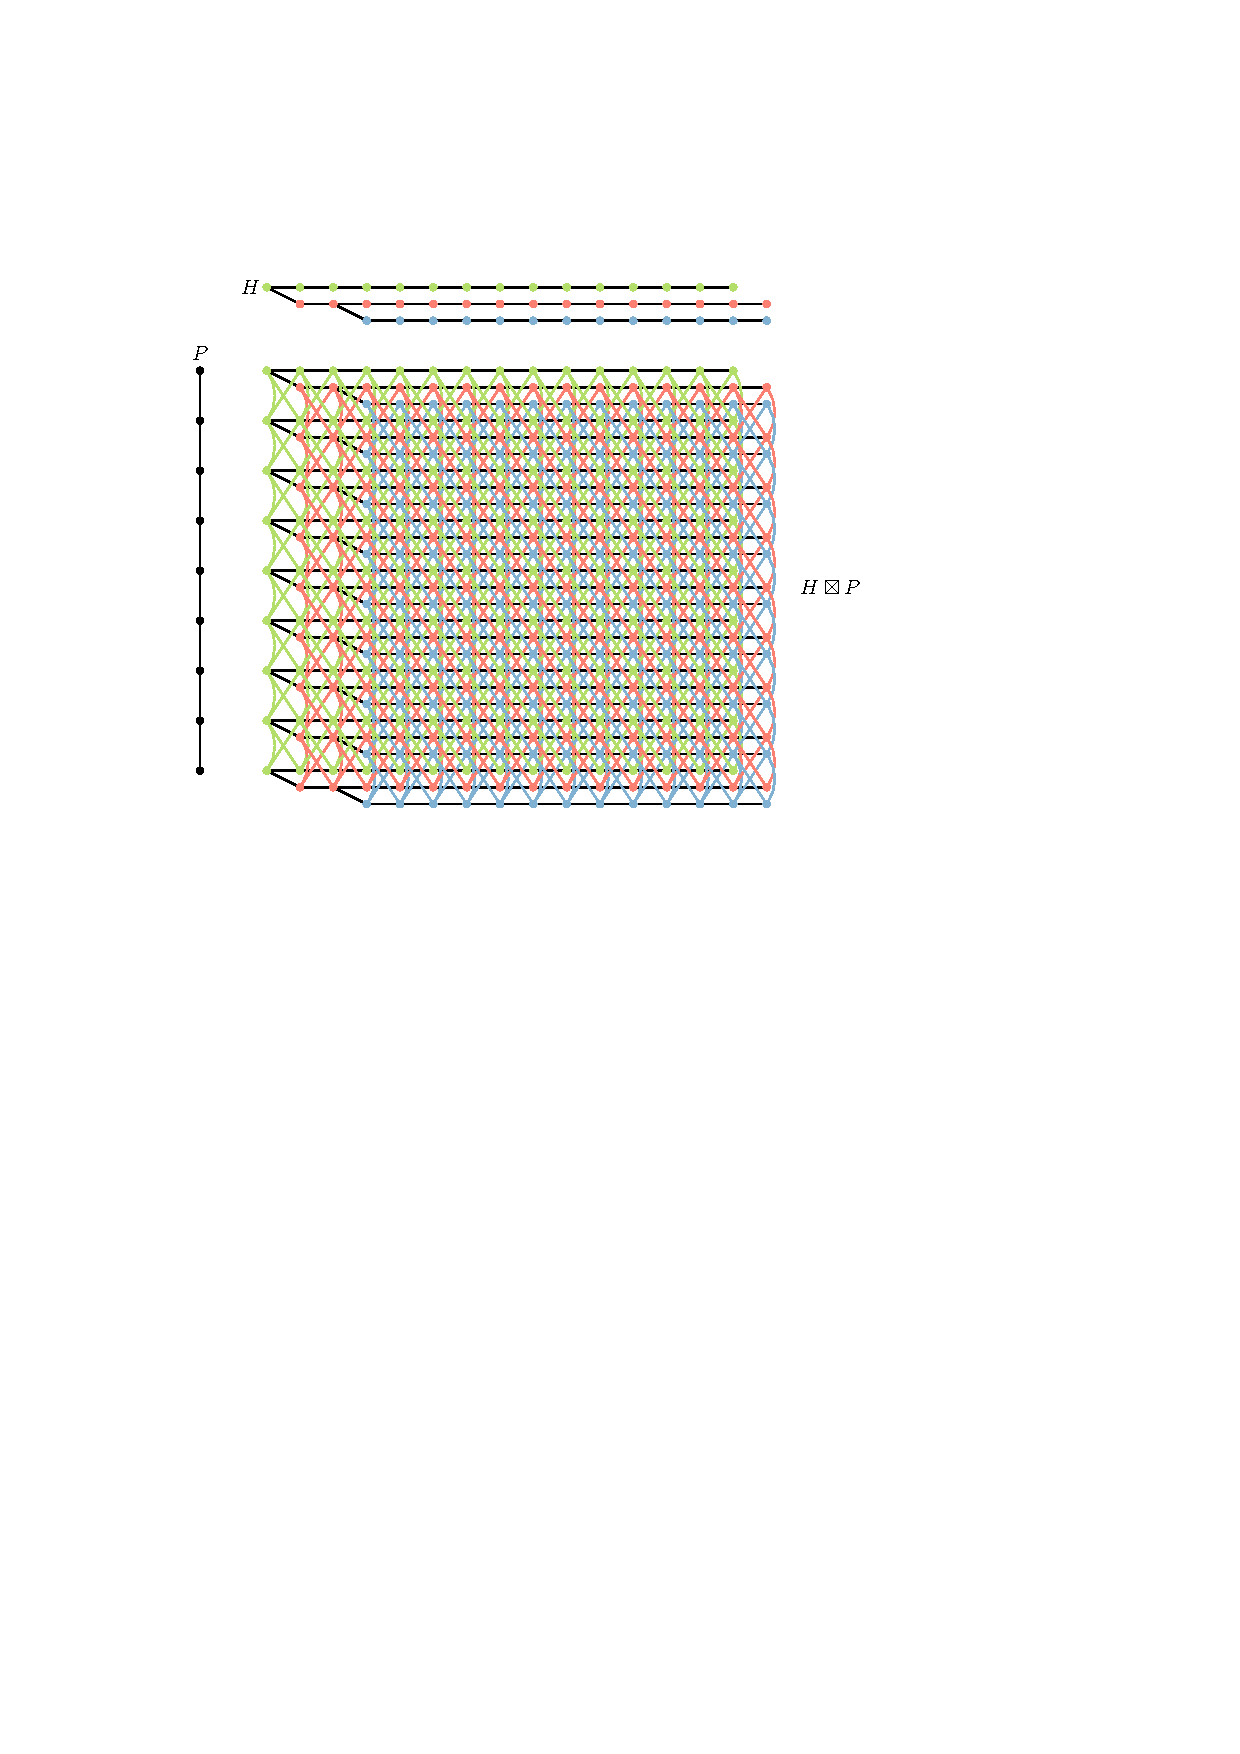
\includegraphics[page=1]{figs/product}
  \caption{The strong product of a tree $H$ and a path $P$.}
  \label{strong_product_fig}
\end{figure}


\subsection{Distance Functions and Metric Spaces}

A \defin{distance function} over a set $S$ is any function $d:S^2\to\R\cup\{\infty\}$ that satisfies $d(x,x)=0$ for all $x\in S$, $d(x,y)\ge 0$ and $d(x,y)=d(y,x)$ for all distinct $x,y\in S$, and $d(x,z) \le d(x,y)+d(y,z)$ for all distinct $x,y,z\in S$.  For any $x\in S$, and any $Z\subseteq S$, $d(x,Z):=\min(\{d(x,y):y\in Z\}\cup\{\infty\})$.  A \defin{metric space} $\mathcal{M}:=(S,d)$ consists of a set $S$ and a distance function $d$ over (some superset of) $S$.
% \gwen{Why some superset of $S$?} \pat{Just because we frequently take ``induced'' metric spaces like $(P,d_2)$ where $P$ is a finite point set in $\R^L$ and $d_2:\R^L\to\R$ is the Euclidean distance function.}
$\mathcal{M}$ is \defin{finite} if $S$ is finite and $\mathcal{M}$ is \defin{non-empty} if $S$ is non-empty.  For $x\in S$ and $r\geq 0$, the \defin{$r$-ball} centered at $x$ is $\mathdefin{B_{\mathcal{M}}(x,r)}:=\{y\in S:d(x,y)\le r\}$.  The \defin{diameter} of a non-empty finite metric space $(S,d)$ is $\mathdefin{\diam_d(S)}:=\max\{d(x,y):x,y\in S\}$, and the
\defin{minimum-distance} of $(S,d)$ is $\mathdefin{\mindist_d(S)}:=\min(\{d(x,y): \{x,y\}\in\binom{S}{2}\}\cup\{\infty\})$.

For any graph $G$, $d_G$ is a distance function over $V(G)$, so $\mathdefin{\mathcal{M}_G}:=(V(G),d_G)$ is a metric space. Any metric space that can be defined this way is referred to as a \defin{graph metric}. For any $S\subseteq V(G)$, the \defin{diameter} and \defin{minimum-distance} of $S$ in $G$ are defined as $\mathdefin{\diam_G(S)}:=\diam_{d_G}(S)$ and $\mathdefin{\mindist_G(S)}:=\mindist_{d_G}(S)$, respectively.


% For $v\in V(G)$ and $W\subseteq V(G)$, $\mathdefin{d_G(v,W)}:=\min\{w\in W:d_G(v,w)\}$.
% The \defin{positive distance in $G$} between $v\in V(G)$ and $W\subseteq V(G)$ is $\mathdefin{d^+_G(v,W)}:=\max\{1,d_G(v,W)\}$.
Since we work with strong products it is worth noting that, for any two graphs $A$ and $B$,
\[
  d_{A\boxtimes B}((x_1,x_2),(y_1,y_2))=\max\{d_A(x_1,y_1),d_B(x_2,y_2)\} \enspace .
\]

The \defin{local density} of a non-empty finite metric space  $\mathcal{M}=(S,d)$
\[
  \mathdefin{\ld(\mathcal{M})}:=\max\{(B_{\mathcal{M}}(x,r)-1)/r:x\in S,\, r>0\}
\]
(this maximum exists because $S$ is finite, so there are only $\binom{|S|}{2}$ values of $r$ that need to be considered).
Thus, if $\mathcal{M}$ has local density at most $D$ then $|B_{\mathcal{M}}(x,r)|\le Dr+1$ for each $x\in S$ and $r\ge 0$.
This definition is consistent with the definition of local density of graphs:  A graph $G$ has local density at most $D$ if and only if the metric space $\mathcal{M}_G$ has local density at most $D$.  Note that, if $(S,d)$ has local density at most $D$ then $(S,d)$ has $\diam_d(S)\ge (|S|-1)/D$ and $\mindist(S)\ge 1/D$.

A \defin{contraction} of a metric space $\mathcal{M}=(S,d)$ into a metric space $\mathcal{M'}=(S',d')$ is a function $\phi:S\to S'$ that satisfies $d'(\phi(x),\phi(y))\le d(x,y)$, for each $x,y\in S$. The \defin{distortion} of $\phi$ is $\max\{d(x,y)/d'(\phi(x),\phi(y)):\{x,y\}\in \binom{S}{2}\}$.\footnote{If there exists $\{x,y\}\in \binom{S}{2}$ with $d(x,y)>0$ and $d'(\phi(x),\phi(y))=0$ then the distortion of $\phi$ is infinite. This will never be the case for any of the contractions we consider in this work.}  When $S\subseteq S'$ and $\phi$ is the identity function we say that $\mathcal{M'}$ is a contraction of $\mathcal{M}$. In particular, saying that $(S,d')$ is a contraction of $(S,d)$ is equivalent to saying that $d'(x,y)\le d(x,y)$ for all $x,y\in S$.

For two points $x,y\in\R^L$, let $\mathdefin{d_2(x,y)}$ denote the Euclidean distance between $x$ and $y$.  A contraction of $(S,d)$ into $(\R^L, d_2)$ for some $L\ge 1$ is called a \defin{Euclidean contraction}.  For $K\subseteq S$ we abuse notation slightly with the shorthand $\mathdefin{\phi(K)}:=\{\phi(x):x\in K\}$.   We make use of two easy observations that follow quickly from these definitions:

\begin{obs}\label{contraction_increases_density}
  Let $\mathcal{M}:=(S,d)$ and $\mathcal{M}':=(S',d')$ be non-empty finite metric spaces.  If $\mathcal{M'}$ has local density $D$ and $\mathcal{M}$ has an injective contraction into $\mathcal{M}'$ then  $\mathcal{M}$ has local density at most $D$.
\end{obs}

\begin{proof}

  Let $\phi:S\to S'$ be an injective contraction of $\mathcal{M}$ into $\mathcal{M}'$.  For every $x\in S$, every $r > 0$, and every $y\in B_\mathcal{M}(x,r)$, we have $d'(\phi(x),\phi(y))\le d(x,y)\le r$, since $\phi$ is a contraction.  Therefore, $B_{\mathcal{M'}}(\phi(x),r)\supseteq \phi(B_{\mathcal{M}}(x,r))$.  Since $\phi$ is injective, $|B_{\mathcal{M'}}(\phi(x),r)|\ge |\phi(B_{\mathcal{M}}(x,r))|=|B_{\mathcal{M}}(x,r)|$.
  Since $\mathcal{M}'$ has local density at most $D$, $rD+1\ge |B_{\mathcal{M'}}(\phi(x),r)|\ge  |B_{\mathcal{M}}(x,r))|$.
\end{proof}

\begin{obs}\label{supergraph_contraction}
  For any graph $I$ and any subgraph $G$ of $I$, $(V(G),d_I)$ is a contraction of $(V(G),d_G)$.
\end{obs}

\begin{proof}
  From the definitions, it follows that $d_I$, restricted to $V(G)$ is a distance function over $V(G)$, so $(V(G),d_I)$ is a metric space.  Since $G$ is a subgraph of $I$, every path in $G$ is also a path in $I$ so, $d_I(x,y)\le d_G(x,y)$ for each $x,y\in V(G)$.  Therefore $(V(G),d_I)$ is a contraction of $(V(G),d_G)$.
\end{proof}

% \begin{obs}
%   If $\phi$ is a $(k,\eta)$-volume-preserving contraction of some metric space $\mathcal{M}$ and $\mathcal{M}$ is contraction of $\mathcal{M}'$
% \end{obs}


\subsection{Volume-Preserving Contractions}
\label{contractions_section}

For a set $K$ of $k\le L+1$ points in $\R^L$, the \defin{Euclidean volume} of $K$, denoted by $\mathdefin{\evol(K)}$, is the $(k-1)$-dimensional volume of the simplex whose vertices are the points in $K$.  For example, if $k=3$, then $\evol(K)$ is the area of the triangle whose vertices are $K$ and that is contained in a plane that contains $K$.

The \defin{ideal volume} of a finite metric space $(K,d)$ is defined as $$\mathdefin{\ivol_d(K)}:=\max\{\evol(\phi(K)):\text{$\phi$ is a Euclidean contraction of $(K,d)$}\}.$$  A Euclidean contraction $\phi:S\to\R^{\ell}$ of a finite metric space $(S,d)$ is \defin{$(k,\eta)$-volume-preserving} if $\evol(\phi(K))\ge \ivol_d(K)/\eta^{k-1}$ for each $k$-element subset $K$ of $S$.  This definition is a generalization of distortion: If $\phi$ is $(2,\eta)$-volume-preserving, then $\phi$ has distortion at most $\eta$.

\citet{feige:approximating} introduces the following definition and theorem as a bridge between ideal volume and Euclidean volume. The \defin{tree volume} of a finite metric space $(K,d)$ is defined as $\mathdefin{\tvol_d(K)}:=\prod_{xy\in E(T)} d(x,y)$ where $T$ is a minimum spanning tree of the weighted complete graph with vertex set $K$ where the weight of each edge $xy$ is equal to $d(x,y)$.  The following lemma makes tree volume a useful intermediate measure when trying to establish that a contraction is volume-preserving.

\begin{lem}[{\citet[Theorem~3]{feige:approximating}}]\label{tvol_vs_ivol}
  Let $(S,d)$ be a finite metric space with $|S|=k$.  Then
  \[
    \ivol_{d}(S) \le \frac{\tvol_d(S)}{(k-1)!} \le 2^{(k-2)/2}\ivol_d(S) \enspace .
  \]
\end{lem}

\subsection{Bandwidth from Local Density and Volume-Preserving Contractions}

The following lemma, whose proof appears in \cref{reciprocal_sum_section}, generalizes \citet[Theorem~10]{feige:approximating} from graph metrics to general metric spaces and establishes a critical connection between local density and tree volume.

\begin{restatable}[{Generalization of \cite[Theorem~10]{feige:approximating}}]{lem}{reciprocalsum}\label{reciprocal_sum}
  For every $n$-element metric space $\mathcal{M}:=(S,d)$ with local density at most $D$ and every positive integer $k$,
  \[
    \sum_{K\in \binom{S}{k}}\frac{1}{\tvol_{d}(K)} < n(DH_n/2)^{k-1} \enspace ,
  \]
  where $\mathdefin{H_n}:=\sum_{i=1}^n 1/i\le 1+\ln n$ is the \defin{$n$-th harmonic number}.
\end{restatable}



\Cref{volume_density_bandwidth}, which appears below and whose proof appears in
\cref{volume_density_bandwidth_section}, is a generalization of \cref{feige_bandwidth_vs_density_graphs} from graph metrics to arbitrary metrics.
 %
 %
 %
 %
 % for graph metrics, although the dependence on the parameters $n$, $D$, $k$, and $\eta$ are not stated explicitly in \cite{feige:approximating}. Here we give a generalization for metric spaces and make the bound on the bandwidth explicit in terms of the parameters $n$, $D$, $k$, and $\eta$.
First, we need a definition of bandwidth for metric spaces.  Let $(S,d)$ be a non-empty finite metric space and let $x_1,\ldots,x_n$ be a permutation of $S$.  Then $\mathdefin{\bw_{(S,d)}(x_1,\ldots,x_n)}:=\max\{j-i:d(x_i,x_j)\le 1,\, 1\le i <j\le n\}$ and $\mathdefin{\bw(S,d)}$ is the minimum of $\bw_{(S,d)}(x_1,\ldots,x_n)$ taken over all $n!$ permutations $x_1,\ldots,x_n$ of $S$.  Note that this coincides with the definition of the bandwidth of a graph: For any connected graph $G$, $\bw(\mathcal{M}_G)=\bw(G)$.  First we observe that injective
%\david{given that `injective' does not appear in the observation, why do we have `injective' here?} \pat{Laziness. In general, a contraction $\phi:A\to B$ of $(A,d_A)$ into $(B,d_B)$ need not be injective, in which case the observation isn't true.  If $B:=\{y\}$ and $\phi(x):=y$ for all $x\in A$ then $\bw(B,d_B)=0$, but this doesn't tell us anything about $\bw(A,d_A)$. The word injective is missing from the statement because saying that $(S,d')$ is a contraction of $(S,d)$ implicitly assumes that we are considering a contraction where $\phi$ is the identity function. I've added (injective) to the statement to remind the reader of this.}
contractions can only increase bandwidth:

%\david{given that `injective' does not appear in the observation, why do we have `injective' here?} \pat{Laziness. In general, a contraction $\phi:A\to B$ of $(A,d_A)$ into $(B,d_B)$ need not be injective, in which case the observation isn't true.  If $B:=\{y\}$ and $\phi(x):=y$ for all $x\in A$ then $\bw(B,d_B)=0$, but this doesn't tell us anything about $\bw(A,d_A)$. The word injective is missing from the statement because saying that $(S,d')$ is a contraction of $(S,d)$ implicitly assumes that we are considering a contraction where $\phi$ is the identity function. I've added (injective) to the statement to remind the reader of this.}

\begin{obs}\label{contraction_increases_bandwidth}
  For every finite metric space $\mathcal{M}:=(S,d)$ and every (injective) contraction $\mathcal{M}':=(S,d')$ of $\mathcal{M}$, $\bw(\mathcal{M}) \le \bw(\mathcal{M}')$.
\end{obs}

\begin{proof}
  Let $x_1,\ldots,x_n$ be an ordering of the elements of $S$ such that $b:=\bw(\mathcal{M}')=\bw_{\mathcal{M}}(x_1,\ldots,x_n)$. Consider any pair of elements $x_ix_j$ with $d(x_i,x_j) \le 1$. Since $\mathcal{M}'$ is a contraction of $\mathcal{M}$, $d'(x_i,x_j)\le 1$.  Since $\bw_{\mathcal{M}'}(x_1,\ldots,x_n)\le b$, $|j-i|\le b$.  Thus $\bw(\mathcal{M})\le \bw_{\mathcal{M}}(x_1,\ldots,x_n)\le b$.
\end{proof}




\begin{restatable}[{Generalization of \cref{feige_bandwidth_vs_density_graphs}}]{thm}{volumedensitybandwidth}\label{volume_density_bandwidth}
  Let $(S,d)$ be a $n$-element metric space with local density at most $D$ and diameter at most $\Delta$.  If $(S,d)$ has a $(k,\eta)$-volume-respecting Euclidean contraction $\phi:S\to\R^L$
  % with $L\ge 4a\ln n$ --- not needed, I think
  then
  \[
    \bw(S,d) \in O((nk\log\Delta)^{1/k}\,Dk\eta\log^{3/2} n) \enspace .
  \]
\end{restatable}






% Let $G$ be a finite graph and let $\mathcal{D}:2^{V(G)}\to[0,1]$ be a probability distribution over subsets of $V(G)$.  Then $\mathcal{D}$ has the \defin{KPR$(\epsilon,\delta,\Delta)$-property} if
% \begin{compactenum}[(i)]
%   \item For each $Z$ in the support of $\mathcal{D}$, each component $C$ of $G-Z$ has $\diam_G(C)< \Delta$.
%   \item For each vertex $v$ of $G$ if we draw $Z$ according to the distribution $\mathcal{D}$, then
%   \[  \Pr(\text{$Z=\emptyset$ or $d_G(v,Z) \ge \floor{\epsilon\Delta})$})\ge \delta \enspace .
%   \]
% \end{compactenum}
% A graph $G$ has the \defin{KPR($\epsilon,\delta)$ property} if, for every positive integer $\Delta$, there exists a distribution $\mathcal{D}_\Delta$ over subsets of $V(G)$ that has the KPR$(\epsilon,\delta,\Delta)$-property.  A family $\mathcal{G}$ of graphs has the \defin{KPR property} if there exists some $\epsilon,\delta>0$ such that every graph in $\mathcal{G}$ has the KPR$(\epsilon,\delta)$ property.
%
% Building on the decomposition of \citet{klein.plotkin.ea:excluded}, \citet{rao:small} shows that planar graphs have the KPR property.  More generally,
%
% \begin{thm}
%   Every $K_{h}$-minor-free graph has the   KPH(\Omega,)
% \end{thm}
%

\subsection{Proof of \cref{main_thm_products}}

We are now ready to prove \cref{main_thm_products}. The structure of our proof is based on the proof of \cref{rao_bandwidth_vs_density} by \citet{rao:small}.
% , which applies to planar graphs and even to $K_{h}$-minor-free graphs for any fixed $h$.  As already noted in the introduction, products of the form $H\boxtimes P$ are not $K_h$-minor-free for any fixed $h$, so Rao's proof cannot be applied directly.
For the remainder of \cref{htimesp_section}, $G$ is an $n$-vertex subgraph of $H\boxtimes P$ where $H$ is a \defin{$t$-tree} (an edge-maximal graph of treewidth $t$) and $P$ is a path.  The proof of \cref{main_thm_products} has the following structure. (We use the notation $\mathcal{M}\rightbroom\mathcal{M'}$ to denote that $\mathcal{M}'$ is a contraction of $\mathcal{M}$.)

\begin{enumerate}
  \item Use a variant of \cref{sparsifier_baker} to find a set $X\subseteq V(H\boxtimes P)$ of size $O(\sqrt{n}\log^2 n)$ such that the metric space $\mathcal{M}:=(V(G-X),d_{(H\boxtimes P)-X})$ has local density $D\in O(\sqrt{n}/\log n)$.  Since $G-X$ is a subgraph of $(H\boxtimes P)-X$, \cref{supergraph_contraction} implies that $\mathcal{M}$ is a contraction of the metric space $\mathcal{M}_{G-X}:=(V(G-X),d_{G-X})$, so $\mathcal{M}_{G-X}\rightbroom\mathcal{M}$.

  \item Design a distance function $d^*:V((H\boxtimes P)-X)^2\to\R$ so that the metric space $\mathcal{M}^*:=(V(H\boxtimes P)\setminus X,d^*)$ is a contraction of $\mathcal{M}$ with the property that the induced metric space $(V(G-X),d^*)$ has local density $O(D)$.

  Graphically, $\mathcal{M}_{G-X}\rightbroom\mathcal{M}\rightbroom\mathcal{M}^*$.

  \item Prove that $\mathcal{M}^*$ has a $(k,O(\sqrt{\log n}))$-volume-preserving Euclidean contraction $\phi:V(G-X)\to\R^L$, for $k\in\Theta(\log n)$.

  \item  By \cref{volume_density_bandwidth},  $\bw(\mathcal{M}^*)\in O(D\log^3 n)=O(\sqrt{n}\log^2 n)$.  Since $\mathcal{M}^*$ is a contraction of $\mathcal{M}_{G-X}$, \cref{contraction_increases_bandwidth} implies that $\bw(G-X)=\bw(\mathcal{M}_{G-X}) \le \bw(\mathcal{M}^*)\in O(\sqrt{n}\log^2 n)$.
\end{enumerate}

The delicate part of the proof is the design of the distance function $d^*$ that contracts $d_{(H\boxtimes P)-X}$ but still ensures that the local density of $(V(G-X),d^*)$ is $O(D)$. If $d^*$ contracts too much, then $(V(G-X),d^*)$ will not have local density $O(D)$. If $d^*$ contracts too little, then it will be difficult to get a $(k,O(\sqrt{\log n}))$-volume-preserving Euclidean embedding. To make this work, we use the structure of the sparsifying set $X$.

\subsection{A Structured Sparsifier}
\label{x_definition}

%\david{This section needs a single lemma that summarises all the required properties of $X$.} \pat{I'll comb through the proof again to see what properties of $\{X_{i,j}:i\in\{0,\ldots,\log N\},j\in\{1,\ldots,N/2^i\}$, in addition to \cref{component_sizes} and \cref{x_size}, are being used.}  \pat{I reread this section, and the only thing we use is \cref{component_sizes}.} \david{OkayI am happy because of the addition at the start of 4.7.}

In this section, we construct a sparsifying set $X$ like that used in \cref{planar_sparsifier}.  The main difference is that we do not use a BFS layering of $G$ when applying \cref{sparsifier_baker}. Instead, we use the layering of $G$ that comes from $H\boxtimes P$.  Although this is really the only difference, we repeat most of the steps in the proof of \cref{sparsifier_baker} in order to establish notations and precisely define the structure of $X$, which will be useful in the design of the distance function $d^*$.  In particular, later sections will rely on the structure of the individual subsets $X_{i,j}$ whose union is $X$.
% \pat{This is a bit repetitive, (it repeats parts in the proof of \cref{sparsifier_baker}), but I think it's better to repeat than to write two parts differently for no reason.  Maybe later we can fold the two proofs together.}

% is a subgraph of $H\boxtimes P$, but with a structure that lends itself to the design of the distance function $d^*$.  The construction is very similar to the construction in the proof of \cref{planar_sparsifier}. The main difference is that we do not apply the separator lemma (\cref{weighted_separator}) directly to a subgraph $G^+_{i,j}$.  Instead, we consider a subgraph $Q^+_{i,j}=H\boxtimes P^+_{i,j}$ of $H\boxtimes P$ that contains $G^+_{i,j}$.  We use this to assign weights to the vertices of $H$ and then apply the separator lemma to $H$ to get a separator $Y_{i,j}$.  In this way, we obtain a `vertical' separators $X_{i,j}:=Y_{i,j}\times V(P^+_{i,j})$.
% For a vertex $v$ in the middle third of $Q^+_{i,j}$, a radius-$2^i$ ball in $(H\boxtimes P)-X$.
%
%
% \pat{Now that I write this, I don't think it's important that the separators in $X_{i,j}$ are vertical.  The important thing is that that distance between a vertex $v$ in the middle-third of $Q^+_{i,j}$ and a vertex $w$ in a different component of $Q^+_{i,j}-X_{i,j}$ is at least $2^i$.  \\[2ex]
% I think our results hold in the following setting:
%  There are fixed $c$ and $t$ such that
%  $G$ has a layering such that, for any $\ell$ and any subgraph $G'$ induced by $\ell$ consecutive layers:  (i)~$\tw(G')\le c\ell$;
%  (ii)~$\textsc{Chop}_{t,\ell}(G')$ always produces a set $W$ such that each component of $G'-W$ has diameter at most $c\ell$.  \\[2ex]
%  I think (ii) might be more easily summarized by arguing that Klein-Plotkin-Rao can be generalized to the setting where $G$ has layered treewidth $t$ using a layering with at most $\Delta$ layers.
%  }

Let $N:=2^{\ceil{\log n}}$ and let $P:=\mathdefin{y_{-N+1},y_{-N+2},\ldots,y_{2N}}$ be a path.  Without loss of generality we assume all vertices of $G$ are contained in $V(H)\times\{y_1,\ldots,y_N\}$.  For each $i\in\{0,\ldots,\log N\}$ and each $j\in\{-1,0,\ldots,N/2^{i}\}$, let $P_{i,j}:=y_{j2^i+1},\ldots,y_{(j+1)2^i}$ be a subpath of $P$ with $2^i$ vertices. For each $i\in\{0,\ldots,\log N\}$ and each $j\in\{0,\ldots,N/2^{i}-1\}$, let $P^+_{i,j}:=P[V(P_{i,j-1})\cup V(P_{i,j})\cup V(P_{i,j+1})]$ be the concatenation of $P_{i,j-1}$, $P_{i,j}$, and $P_{i,j+1}$. Define $Q_{i,j}\coloneqq H\boxtimes P_{i,j}$ and $Q^+_{i,j}\coloneqq H\boxtimes P^+_{i,j}$.
In words, $Q_{i,0},\ldots,Q_{i,N/2^i-1}$ partitions the part of $H\boxtimes P$ that contains $G$ into vertex-disjoint strips of height $2^i$. The subgraph $Q^+_{i,j}$ is a strip of height $3\cdot 2^i$ that contains $Q_{i,j}$ in its middle third.
% Observe that, for each $i\in\{1,\ldots,\log N\}$ and $j\in\{0,\ldots,N/2^i-1\}$, each of the graphs $Q^+_{i-1,2j}$ and $Q^+_{i-1,2j+1}$ is a subgraph of $Q^+_{i,j}$. Equivalently, $Q^+_{i,j}$ is a subgraph of $Q_{i+1,\lfloor j/2\rfloor}$ for each $i\in\{0,\ldots,\log N-1\}$ and each $j\in\{0,\ldots,N/2^i-1\}$.

To construct our sparsifying set $X$, we first construct vertex subsets $Y_{i,j}$ of $H$ for each $i\in\{0,1,\ldots,\log N\}$ and $j\in\{0,\ldots,N/2^{i}-1\}$.  Define the weight function $\xi_{i,j}:V(H)\to\N$ where $\xi_{i,j}(x):=|(\{x\}\times V(P^+_{i,j})) \cap V(G)|$.  Observe that $\xi_{i,j}(H):=\sum_{x\in V(H)} \xi_{i,j}(x)=|V(Q^+_{i,j})\cap V(G)|$. Let $D\ge 2$ be a real number.  By \cref{weighted_separator} with $c:=\lceil\xi_{i,j}(H)/2^{i-1}D\rceil$, there exists $Y_{i,j}\subseteq V(H)$ of size at most $(t+1)\xi_{i,j}(H)/(2^{i-1}D)$, such that each component $C$ of $H-Y_{i,j}$ has total weight $\xi_{i,j}(C)\le 2^{i-1}D$.  For each $i\in\{0,1,\ldots,\log N\}$ and $j\in\{0,\ldots,N/2^{i}-1\}$, let $\mathdefin{X_{i,j}}:=Y_{i,j}\times V(P^+_{i,j})$.  We think of $X_{i,j}$ as a vertical separator that splits the strip $Q^+_{i,j}$ into parts using vertex cuts that run from the top to the bottom of $Q^+_{i,j}$.

\begin{lem}\label{component_sizes}
  For each $i\in\{0,,\ldots,\log N\}$ and $j\in\{0,\ldots,N/2^{i}-1\}$, each component of $Q^+_{i,j}-X_{i,j}$ has at most $2^{i-1}D$ vertices.\
\end{lem}

\begin{proof}
  The number of vertices of $G$ in a component $C$ of $Q^+_{i,j}-X_{i,j}$ is equal to the total weight $\zeta_{i,j}(C_H)$ of the corresponding component $C_H$ of $H-Y_{i,j}$.  Therefore, each component of $Q^+_{i,j}-X_{i,j}$ contains at most $2^{i-1}D$ vertices of $G$.
\end{proof}

Let $\mathdefin{X}:=\bigcup_{i=0}^{\log N}\bigcup_{j=0}^{N/2^i-1} X_{i,j}$.

\begin{lem}\label{x_size}
  $|X|\le (18(t+1)n/D)(1+\log N)$.
\end{lem}

\begin{proof}
  Observe that $\sum_{j=0}^{N/2^i-1} \xi_{i,j}(H)\le\sum_{j=0}^{N/2^i-1} 3|V(G_{i,j})| \le 3n$, since, each vertex $v$ of $G$ can only appear in $Q^+_{i,j-1}, Q^+_{i,j}$, and $Q^+_{i,j+1}$ where $j$ is the unique index such that $v\in V(Q_{i,j})$.    By definition, $|X_{i,j}|=3\cdot 2^i \cdot |Y_{i,j}| \le 6(t+1)\xi_{i,j}(H)/D$.  Therefore, $\sum_{j=0}^{N/2^i-1} |X_{i,j}|\le 18(t+1)n/D$. Summing over $i\in\{0,\ldots,\log N\}$ completes the proof.
  % Any subpath $P':=y_{q+1},\ldots,y_{q+\ell}$ of $P$ is contained in $P^+_{i,j}$ for $i:=\lceil\log \ell\rceil$ and $j=\lfloor(q+1)/2^i\rfloor$.  Therefore $H\boxtimes P'$ is contained in $Q^+_{i,j}$.  Therefore, each component of $(H\boxtimes P')-X$ is contained in a component of $Q_{i,j}-X_{i,j}$.  Therefore, each component of $(H\boxtimes P')-X$ contains at most $D2^{i-1}\le D\ell$ vertices of $G$.
\end{proof}

\subsection{\boldmath The Distance Function $d^*$}
\label{d_star_definition}

In order to construct a volume-preserving Euclidean contraction $\phi$ for a distance function $d$ we must ensure (at least) that $d_2(\phi(v),\phi(w))$ is large whenever $d(v,w)$ is large.  This is relatively easy to do for the distance function $d_{H\boxtimes P}$ using (simplifications of) the techniques used by \citet{rao:small} for planar graphs. This is more difficult for $d_{(H\boxtimes P)-X}$ because distances are larger, which only makes the problem harder.  Some of these distances are necessarily large; the obstacles in $X$ are needed to ensure that $(V(G),d_{(H\boxtimes P)-X})$ has local density at most $D$.  The purpose of a single set $X_{i,j}$ is to increase distances between some pairs of vertices in $Q^+_{i,j}$ so that they are at least $2^i$.  However, the obstacles in $X$ sometimes interact, by chance, to make distances excessively large. \cref{big_distance} shows that, even when $H=P$, obstacles in $X_{i,j+1}$ and in $X_{i,j-1}$ can interact in such a way that $d_{(H\boxtimes P)-X}(v,w)$ can become $r2^i$ for arbitrarily large $r$.  This large distance is not needed to ensure the local density bound and it makes it difficult to construct a volume-preserving Euclidean contraction of $(V(G),d_{(H\boxtimes P)-X})$.  The purpose of the intermediate distance function $d^*$ is to reduce these unnecessarily large distances so that $d^*(v,w)$ is defined only by the ``worst'' obstacle in $X$ that separates $v$ and $w$.


 % in such a way that the local density of $\mathcal{M}^*:=(V(G),d^*)$ is $O(D)$ but it is easier to find a volume-preserving Euclidean contraction of $\mathcal{M}^*$ than to find one of $(V(G),d_{(H\boxtimes P)-X})$. Some elements in the definition of $d^*$ are illustrated in \cref{d_star}.


\begin{figure}
  \centering
  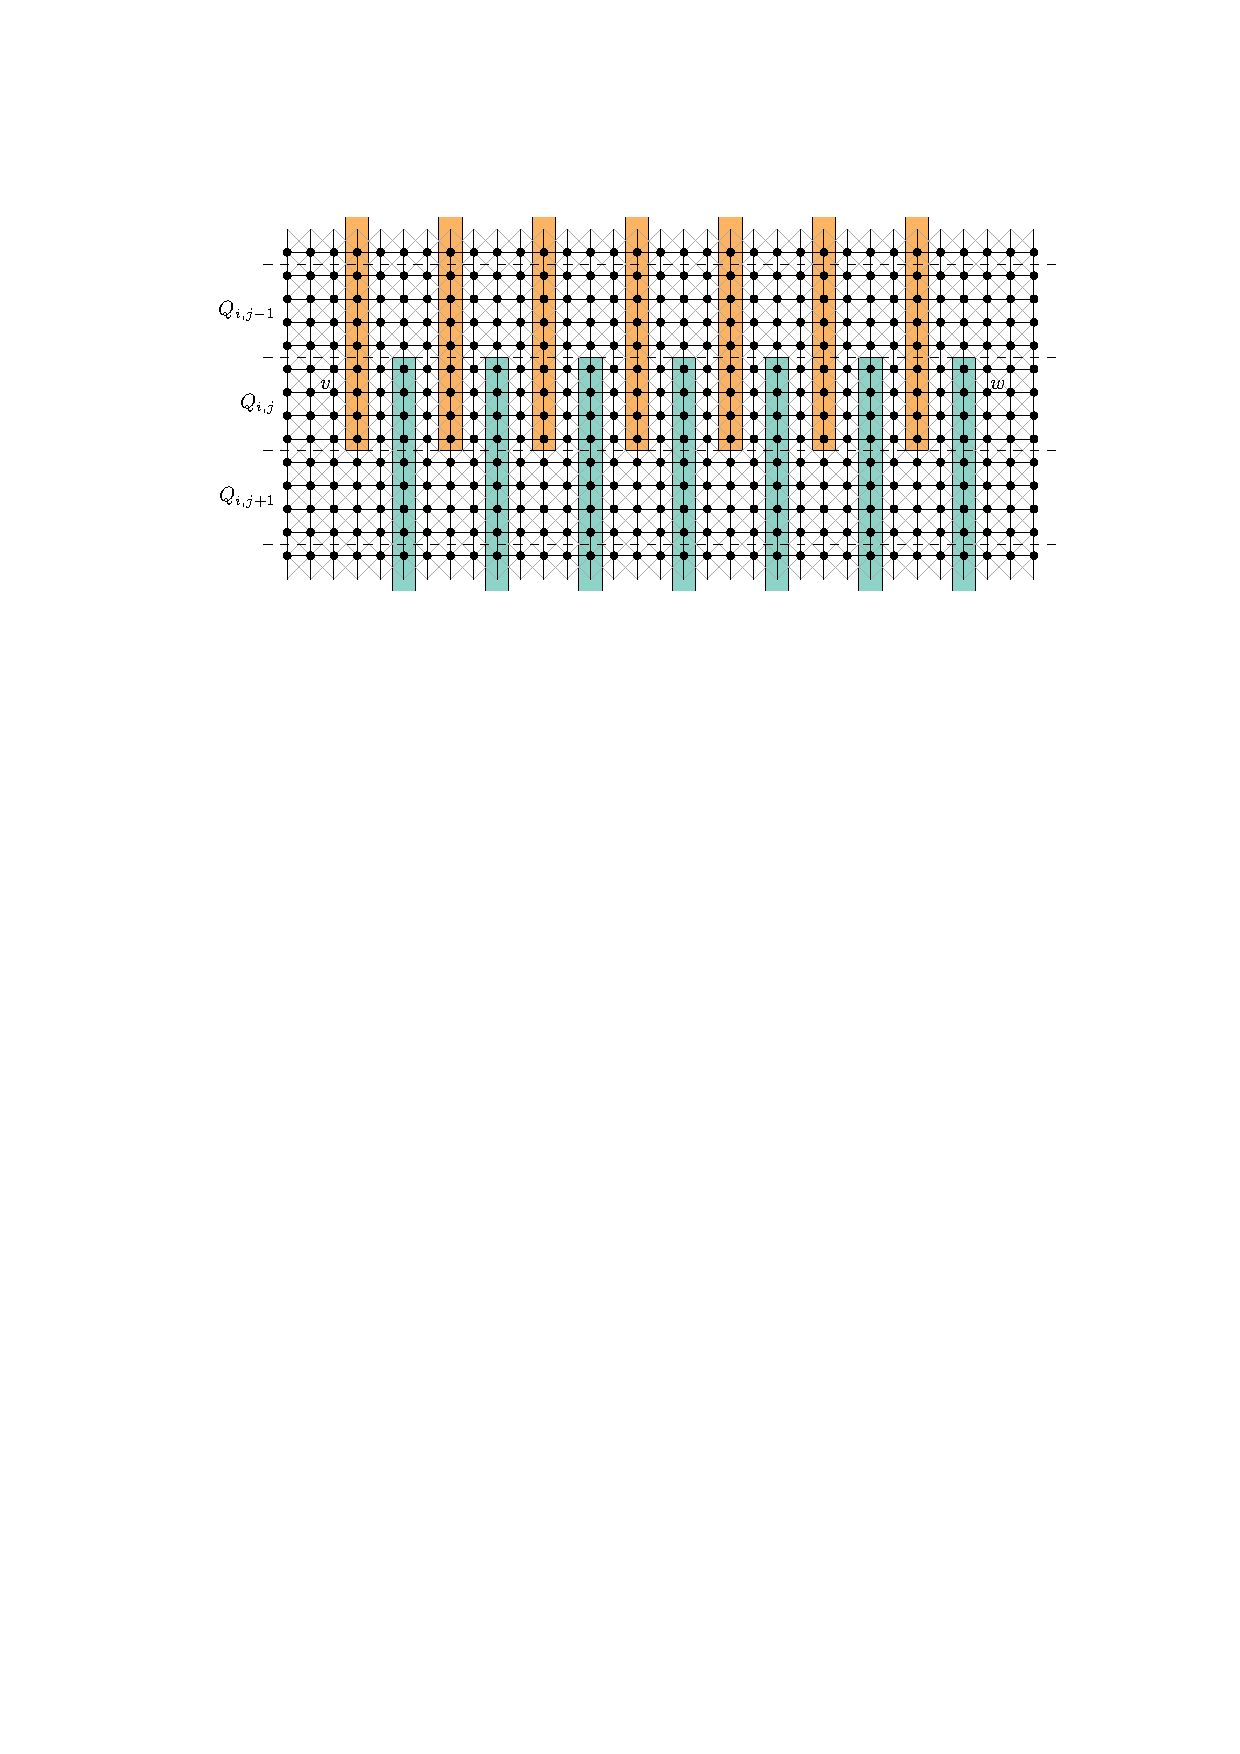
\includegraphics{figs/bad_combination}
  \caption{Obstacles not in $X_{i,j}$ can interact to create excessively large distances between vertices in $Q_{i,j}$.}
  \label{big_distance}
\end{figure}



For any subgraph of $A'$ of a graph $A$, we use the shorthand $\overline{A}':=V(A)\setminus V(A')$. (When we use this notation, the graph $A$ will be clear from context.)
% For a graph $G$, a vertex $v$ of $G$ and a subgraph $C$ of $G$, we use the shorthand $\mathdefin{d_G(v,\overline{C})}:=d_G(v,V(G)\setminus V(C))$.
For any vertex $u$ of $H\boxtimes P$, let $u_P$ denote the second coordinate of $u$ (the projection of $u$ onto $P$).  Let $u$ and $v$ be two vertices of $(H\boxtimes P)-X$.  If $u$ and $v$ are both vertices of $Q^+_{i,j}$ but are in different components of $Q^+_{i,j}-X_{i,j}$, then define
\[
  d_{i,j}(u,v):=\min \{d_P(u_P,x) + d_P(x,v_P):x\in \overline{P}^+_{i,j}\} \enspace .
\]
Otherwise (if one of $u$ or $v$ is not in $Q^+_{i,j}$ or $u$ and $v$ are in the same component of $Q^+_{i,j}-X_{i,j}$), define $d_{i,j}(u,v)=0$.  When $d_{i,j}(u,v)>0$, it is helpful to think of $d_{i,j}(u,v)$ as the length of the shortest walk in $P$ that begins at $u_P$, leaves $P^+_{i,j}$ and returns to $v_P$.  Now define our distance function
\[
  d^*(u,v):=\max\left(\{d_{H\boxtimes P}(u,v)\}\cup \left\{d_{i,j}(u,v):(i,j)\in\{0,\ldots,\log N\}\times\{1,\ldots,N/2^i-1\}\right\}\right)
\]
Intuitively, $d^*(u,v)$ captures the fact that any path from $u$ to $v$ in $(H\boxtimes P)-X$ must navigate around each obstacle $X_{i,j}$ that separates $u$ and $v$ in the graph $Q^+_{i,j}$.  At the very least, this requires a path from $u$ to some vertex $x$ outside of $Q^+_{i,j}$ followed by a path from $x$ to $v$.  The length of this path is at least the length of the shortest walk in $P$ that begins at $u_P$, contains $x_P$ and ends at $w_P$.

\begin{lem}\label{d_star_distance}
  The function $d^*:V((H\boxtimes P)-X)\to\N\cup\{\infty\}$ is a distance function for $V((H\boxtimes P)-X)$.
\end{lem}

\begin{proof}
  It is straightforward to verify that $d^*(u,u)=0$ for all $u\in V((H\boxtimes P)\setminus X)$ and that $d^*(u,v)=d(v,u)\ge 0$ for all $u,v\in V((H\boxtimes P)-X)$.  It only remains to verify that $d^*$ satisfies the triangle inequality.  We must show that, for distinct $u,v,w\in V((H\boxtimes P)-X)$, $d^*(u,w)\le d^*(u,v)+d^*(v,w)$.

  If $d^*(u,w)=0$ then $d^*(u,v)+d^*(v,w)\ge 0=d^*(u,w)$ and we are done.  If $d^*(u,w)=d_{H\boxtimes P}(u,w)$ then $d^*(u,v)+d^*(v,w)\ge d_{H\boxtimes P}(u,v)+d_{H\boxtimes P}(v,w)\ge d_{H\boxtimes P}(u,w)$ and we are also done.  Otherwise, $d^*(u,w)=d_{i,j}(u,w)>0$ for some $i,j$.  Then $u$ and $w$ are vertices of $Q^+_{i,j}$ that are in different components of $Q^+_{i,j}-X_{i,j}$.  There are two cases to consider, depending on the location of $v$:
  \begin{compactenum}
    \item If $v\not\in V(Q^+_{i,j})$ then $d^*(u,v)+d^*(v,w)\ge d_{H\boxtimes P}(u,v)+d_{H\boxtimes P}(v,w) \ge d_P(u_P,v_P)+d_P(v_P,w_P)\ge d_{i,j}(u,w)=d^*(u,w)$.

    \item If $v\in V(Q^+_{i,j})$ then, since $u$ and $w$ are in different components $C_u$ and $C_w$ of $Q^+_{i,j}-X_{i,j}$, at least one of $C_u$ or $C_w$ does not contain $v$.  Without loss of generality, suppose $C_w$ does not contain $v$.  Then $d^*(u,v)+d^*(v,w)\ge d_{H\boxtimes P}(u,v)+d_{i,j}(v,w) \ge d_{P}(u_P,v_P)+d_{i,j}(v,w)$.  Now, $d_{P}(u_P,v_P)$ is the length of a path in $P$ from $u_P$ to $v_P$ and $d_{i,j}(v,w)$ is the length of a (shortest) walk in $P$ that begins at $v_P$, leaves $P^+_{i,j}$ and then returns to $w_P$. Thus,   $d_{P}(u_P,v_P)+d_{i,j}(v,w)$ is the length of a walk in $P$ that begins at $u_P$, leaves $P^+_{i,j}$ and then returns to $w_P$. On the other hand, $d_{i,j}(u,w)$ is the length of a shortest walk in $P$ that begins at $u_P$, leaves $P^+_{i,j}$ and returns to $w_P$, so $d_{i,j}(u,w)\le d_P(u_P,v_P)+d_{i,j}(v,w)$.  Therefore, $d^*(u,v)+d^*(v,w)\ge d_{P}(u_P,v_P)+d_{i,j}(v,w)\ge d_{i,j}(u,w)=d^*(u,w)$. \qedhere
  \end{compactenum}
\end{proof}


\begin{lem}\label{delta_density}
  The metric space $\mathcal{M}^*:=(V(G-X),d^*)$ has local density at most $D$.
\end{lem}

\begin{proof}
  We must show that, for any $v\in V(G)$ and any $r>0$, $|B_{\mathcal{M}^*}(v,r)|\le Dr+1$.  If $r\ge n/D$ then this is trivial, so assume that $r\le n/D$.  Consider some vertex $w\in B_{\mathcal{M}^*}(v,r)$.  Let $i:=\lceil\log r\rceil$ and let $j$ be such that $v$ is a vertex of $Q_{i,j}$.  Since $w\in B_{\mathcal{M}^*}(v,r)$, $d_{H\boxtimes P}(v,w)\le r\le 2^i$.  Therefore $d_P(v_P,w_P)\le d_{H\boxtimes P}(v,w)\le 2^i$.  Therefore $w$ is contained in $Q^+_{i,j}$.  Since $d^*(v,w)\le r$, $d_{i,j}(v,w)\le r$.  This implies that $v$ and $w$ are in the same component of $Q^+_{i,j}-X_{i,j}$ since, otherwise, $d_{i,j}(v,w)\ge d_P(u_P,\overline{P}^+_{i,j}) + d_P(\overline{P}^+_{i,j},w_P)\ge 2^i+1$.
  Therefore, $B_{\mathcal{M}^*}(v,r)$ is contained in the component $C$ of $Q^+_{i,j}-X_{i,j}$ that contains $v$.  By \cref{component_sizes}, $|V(C)|\le 2^{i-1}D< rD$.  Therefore, $|B_{\mathcal{M}^*}(v,r)|\le |V(C)|< rD$.
\end{proof}

\begin{lem}
  The metric space $(V((H\boxtimes P)-X),d^*)$ is a contraction of $\mathcal{M}_{(H\boxtimes P)-X}=(V((H\boxtimes P)-X),d_{(H\boxtimes P)-X})$.
\end{lem}

\begin{proof}
  Let $u$ and $v$ be distinct vertices of $(H\boxtimes P)-X$.  If $d^*(u,v)=d_{H\boxtimes P}(u,v)$ then, $d^*(u,v)=d_{H\boxtimes P}(u,v)\le d_{(H\boxtimes P)-X}(u,v)$.  If $d^*(u,v)=d_{i,j}(u,v)$ for some $i$ and $j$ then any path from $u$ to $v$ in $(H\boxtimes P)-X$ must contain some vertex $x$ not in $Q^+_{i,j}$ since $u$ and $v$ are in different components of $Q^+_{i,j}-X$.  The shortest such path has length at least $d_{H\boxtimes P}(u,x)+d_{H\boxtimes P}(x,v) \ge d_P(u_P,x_P)+d_P(x_P,v_P) \ge d_{i,j}(u,v)=d^*(u,v)$.
\end{proof}

The preceding lemmas are summarized in the following corollary:

\begin{cor}\label{d_star_summary}
  The metric space $(V((H\boxtimes P)-X), d^*)$ is a  contraction of $(V((H\boxtimes P)-X), d_{(H\boxtimes P)-X})$ and the metric space $(V(G-X),d^*)$ has local density at most $D$.
\end{cor}



\subsection{Volume-Preserving Contraction of $\mathcal{M}^*$}

Recall that, throughout this section, $G$ is an $n$-vertex subgraph of $H\boxtimes P$ where $H$ is a $t$-tree. The path $P$ and the set $X:=\bigcup_{i=0}^{\log N}\bigcup_{j=0}^{N/2^i-1} X_{i,j}$ are defined as in \cref{x_definition}.  The distance function $d^*:V((H\boxtimes P)-X)\to\R$ is defined as in \cref{d_star_definition}.  In this subsection we prove the following result:
% \david{At this point, we should say what assumptions we are making about $G$ and $H\boxtimes P$, and say that  $X$ is from Lemma~???.}

% \gwen{The proof is actually given in \cref{Euclidean_embedding_section}.}
% \pat{I changed these to subsections}

\begin{lem}\label{dstar_contraction}
For every integer $k\in\{2,\ldots,n\}$, the metric space $\mathcal{M}^*:=(V(G-X),d^*)$ has a $(k,O(\sqrt{\log n}))$-volume-preserving Euclidean contraction.
\end{lem}

\subsubsection{Decomposing $H\boxtimes P$}

Let $\Delta\ge 4$ be a power of $2$. We now show how to randomly decompose $H\boxtimes P$ into subgraphs $\{(H\boxtimes P)^\Delta_{a,b}:(a,b)\in\Z^2\}$. The only randomness in this decomposition comes from choosing two independent uniformly random integers $r_H$ and $r_P$ in $\{0,\ldots,\Delta-1\}$. See \cref{chop_fig}, for an example.

\begin{figure}
  \centering
  \includegraphics[page=2]{figs/product}
  \caption{The result of decomposing the graph $H\boxtimes P$ in \cref{strong_product_fig} with $\Delta=4$, $r_H=2$, and $r_P=3$.}
  \label{chop_fig}
\end{figure}

Let $\{L_s:s\in\Z\}$ be a BFS layering of $H$.  For each integer $a$, let $H^\Delta_a:=H[\bigcup_{s=r_H+a\Delta}^{r_H+(a+1)\Delta-1} L_s]$ so that $\{H^\Delta_a:a\in \Z\}$ is a pairwise vertex-disjoint collection of induced subgraphs that covers $V(H)$ and each $H^\Delta_a$ is a subgraph of $H$ induced by $\Delta$ consecutive BFS layers. For each integer $b$, let $P^\Delta_b:=P[\{y_{r_P+b\Delta},\ldots,y_{r_P+(b+1)\Delta-1}]$ so that $\{P^\Delta_b:b\in\Z\}$ is a collection of vertex disjoint paths, each having $\Delta$ vertices, that cover $P$.   For each $(a,b)\in\Z^2$, let $(H\boxtimes P)^\Delta_{a,b}:= H^\Delta_a \boxtimes P^\Delta_b$.

\david{Given that the following lemmas are not self-contained, I suggest it would be better to call them claims. }

\begin{lem}\label{component_diameter}
  For each $(a,b)\in\Z^2$, each component $C$ of $(H\boxtimes P)^\Delta_{a,b}$ has $\diam_{H\boxtimes P}(C)\le 2\Delta+1$.
\end{lem}

\begin{proof}
  Let $v:=(v_1,v_2)$ and $w:=(w_1,w_2)$ be two vertices of $(H\boxtimes P)^\Delta_{a,b}$.  Our task is to show that $d_{H\boxtimes P}(v,w)\le 2\Delta+1$.  Recall that
  $d_{H\boxtimes P}(v,w)=\max\{d_{H}(v_1,w_1),d_{P}(v_2,w_2)\}$.  Since $P^\Delta_b$ is a subpath of $P$ with $\Delta$ vertices, $d_P(v_2,w_2)=d_{P^\Delta_b}(v_2,w_2)\le\Delta-1$, so we need only upper bound $d_{H}(v_1,w_1)$.

  To do this, we make use of the following property of BFS layerings of $t$-trees \cite{KP08,DMW05}:  For every integer $s$,
  for each component $C$ of $H[L_{s+1}]$,
    the set $N_C$ of vertices in $L_{s}$ that are adjacent to at least one vertex in $C$ form a clique in $H$.
  Since $v_1$ and $w_1$ are in the same component $A$ of $H^\Delta_a$, this implies that $C:=A[L_{r_H+a\Delta}]$ is connected.  This implies that the set $N_C$ of vertices in $L_{r_H+a\Delta-1}$ adjacent to vertices in $C$ form a clique.  Then $H^\Delta_a$ contains a path of length at most $\Delta$ from $v_1$ to a vertex $v_1'$ in $N_C$.   Likewise, $H^\Delta_a$ contains a path of length at most $\Delta$ from $w$ to a vertex $w'$ in $N_C$. Since $N_C$ is clique $v'=w'$ or $v'$ and $w'$ are adjacent.  In the former case, there is a path in $H$ from $v$ to $w$ of length at most $2\Delta$. In the latter case there is a path from $v$ to $w$ of length at most $2\Delta+1$.
\end{proof}

\begin{lem}\label{good_probability}
  Fix some vertex $v$ of $H\boxtimes P$ independently of $r_H$ and $r_P$ and let $(a,b)$ be such that $v$ is a vertex of $(H\boxtimes P)^\Delta_{a,b}$.  Then, with probability at least $1/4$,  $d_{H\boxtimes P}(v, V(H\boxtimes P)\setminus V((H\boxtimes P)^\Delta_{a,b})) \ge \Delta/4$.
\end{lem}

\begin{proof}
  Let $v:=(v_1,v_2)$.
  % and let $H'$ be the component of $H_{a}$ that contains $v_1$, so $C:=H'\boxtimes P_b$ is the component of $(H\boxtimes P)^\Delta_{a,b}$ that contains $v$.
  Let $\mathcal{E}$ be the event $d_{H\boxtimes P}(v, V(H\boxtimes P)\setminus V((H\boxtimes P)_{a,b}^\Delta)) \ge \Delta/4$, let $\mathcal{E}_H$ be the event $d_{H}(v_1, V(H)\setminus V(H^\Delta_a))\ge\Delta/4$ and let $\mathcal{E}_P$ be the event $d_{P}(v_2, V(P)\setminus V(P^\Delta_b))\ge\Delta/4$.  Then $\mathcal{E}=\mathcal{E}_H\cap\mathcal{E}_P$.

  Recall that our partition is defined in terms of a BFS layering $\{L_i:i\in\Z\}$ of $H$ and a random offset $r_H\in\{0,\ldots,\Delta-1\}$.
  The complementary event $\overline{\mathcal{E}}_H$ occurs if and only if $(i\bmod\Delta)-r_H\in\{-\Delta/4-1,\ldots,\Delta/4-1\}$. The number of such $r_H$ is $\Delta/2-1$, so $\Pr(\overline{\mathcal{E}}_H)=(\Delta/2-1)/\Delta < 1/2$ and $\Pr(\mathcal{E}_H)>1/2$.  Similarly $\overline{\mathcal{E}}_P$ occurs if and only if $v_2=y_j$ and $|(j\bmod\Delta)-r_P|\in\{-\Delta/4-1,\ldots,\Delta/4-1\}$ which also occurs with probability less than $1/2$, so $\Pr(\mathcal{E}_P)> 1/2$.

  The events $\mathcal{E}_H$ and $\mathcal{E}_P$ are independent since $\mathcal{E}_H$ depends only on the choice of $r_H$ and $\mathcal{E}_P$ depends only on the choice of $r_P$.
  Therefore $\Pr(\mathcal{E})=\Pr(\mathcal{E}_H)\cdot\Pr(\mathcal{E}_P) > 1/4$.
\end{proof}



% \subsection{Decomposing $H$: The Klein-Plotkin-Rao Partition}
%
% \pat{The next two sections can be simplified.  We can assume $H$ is a $t$-tree.  Then doing BFS in $H$ and chopping one out of every $\Delta$ layers breaks $H$ into components of weak diameter at most $2\Delta$ (by shadow completeness).  Then you chop $P$ as before, which breaks $H\boxtimes P$ into components of weak diameter at most $2\Delta$.}
%
%
% First, fix some integer $\Delta \ge 1$.
% Consider the following random process that, given a connected graph $H$ constructs a random subset $\mathdefin{\textsc{Chop}_{\Delta,t}(H)}$ of vertices in $H$. If $t=0$ then $\textsc{Chop}_{\Delta,0}(H):=\emptyset$.  Otherwise, select any vertex $x$ in $H$ and choose a uniformly random $r\in\{0,\ldots,\Delta-1\}$.  Let $R:=\{y\in V(H):d_{H}(x,y)\equiv r\pmod{\Delta}\}$ and let $C_1,\ldots,C_m$ be the connected components of $H-R$.  Then $\textsc{Chop}_{\Delta,t}(H):=R\cup\bigcup_{i=1}^m \textsc{Chop}_{\Delta,t-1}(C_i)$.
%
%
% The following lemma, with a greater dependence on $t$, is due to \citet{klein.plotkin.ea:excluded}. The version shown here was proved by \citet{fakcharoenphol.talwar:improved}. The presentation here closely follows that of \citet{lee:simpler}.
%
% \begin{lem}[{\citet{klein.plotkin.ea:excluded,fakcharoenphol.talwar:improved,lee:simpler}}]\label{component_diameter_h}
%   If $H$ is a connected $K_{t+1}$-minor-free graph then each component $C$ of $H-\textsc{Chop}_{\Delta,t}(H)$ has $\diam_H(C)\le 16t\Delta$.
% \end{lem}
%
%
% % Say that a vertex $x$ of $H$ is \defin{$\delta$-good} with respect to a set $X\substeq V(H)$ if $d_{H}(x,X)\ge \delta$ and $x$ is \defin{$\delta$-bad} with respect to $X$ otherwise.
%
% % In the following lemma, and for the rest of this section, we use the convention that for any vertex $x$ of $H$, $d_H(x,\emptyset):=\infty$.
%
% \begin{lem}\label{delta_bad_h}
%   For any vertex $x$ of $H$ and any integer $\delta\ge 1$, $$\Pr(d_H(x, \textsc{Chop}_{\Delta,t}(H)< \delta)\le t\,(2\delta-1)/\Delta.$$
% \end{lem}
%
% \begin{proof}
%   The proof is by induction on $t$. If $d_H(x,\textsc{Chop}_{\Delta,t}(H) < \delta)$ then $d(x,R)< \delta$ or, if $t>1$,  $d_H(x,\textsc{Chop}_{\Delta,t-1}(C) < \delta)$ where $C$ is the component of $H-R$ that contains $x$.  Since there are at most $2\delta-1$ choices of $r$ for which $d_H(x,R)<\delta$, $\Pr(d_H(x,R)<\delta) \le (2\delta-1)/\Delta$. For $t=1$, this completes the proof.  For $t>1$, the proof follows from the inductive hypothesis on $\textsc{Chop}_{\Delta,t-1}(C)$ and the union bound.
% \end{proof}
%
% \subsection{\boldmath Decomposing $H\boxtimes P$}
%
% % Let $G$ be a subgraph of $H\boxtimes P$ where $P:=y_1,\ldots,y_h$.
%
% Choose a uniformly random $r_0\in\{0,\ldots,\Delta-1\}$, let $Y_0:=Y_{0,\Delta,t}(P):=\{y_i\in V(P):i\equiv r_0\pmod\Delta\}$ and let $Y:=Y_{\Delta,t}(P):=V(H)\times Y_0$.  Let $W_0\subseteq V(H)$ be the set obtained by executing $\textsc{Chop}_{\Delta,t}(H)$, let $W:=W_0\times V(P)$ and let $Z:=\mathdefin{Z_{\Delta,t}(H,P)}:=W\cup Y$.
%
% % For some intuition, it is helpful to consider the case when $H$ is a path and $t=1$.  In this case, $H\boxtimes P$ is a grid with diagonal edges.  Starting from row $r\in\{0,\ldots,\Delta-1\}$, the set $Y$ contains one out of every $\Delta$ rows of this grid.  Each of the components $C_1,\ldots,C_m$ of $H\boxtimes P-Y$, except the top-most, $C_1$ and bottom-most, $C_m$ is a grid with $\Delta-1$ rows.  For each component $C_i$, the set $X$ contains one out of every $\Delta$ columns of $C_i$, starting from column $r_i\in\{0,\ldots,\Delta-1\}$. \todo{Add figure}
%
% \begin{lem}\label{component_diameter}
%   If $H$ is $K_{t+1}$-minor-free, then each component $C$ of $H\boxtimes P-Z$ has $\diam_{H\boxtimes P}(C)\le ?t\Delta$.
% \end{lem}
%
% \begin{proof}
%   Let $C$ be a component of $H\boxtimes P-Z$.  For any two vertices $x:=(x_1,x_2)$ and $y:=(y_1,y_2)$ of $C$, $d_{H\boxtimes P}(x,y) = \max\{d_{H}(x_1,y_1),d_{P}(x_2,y_2)$. By \cref{component_diameter_h},  $d_{H\boxtimes P}(x_1,y_1)\le ?t\Delta$.  By the choice of $Y_0$, $d_{P}(x,y)<\Delta$.
% \end{proof}
%
% \begin{lem}\label{delta_bad_product}
%   For any vertex $x$ of $H\boxtimes P$ and any integer $\delta\ge 1$, $$\Pr(d_{H\boxtimes P}(x,Z)< \delta)\le (t+1)(2\delta-1)/\Delta.$$
% \end{lem}
%
% \begin{proof}
%   If $d_{H\boxtimes P}(x,Z)<\delta$ then $d_{H\boxtimes P}(x,Y)<\delta$ or $d_{C}(x,Z)<\delta$ where $C$ is the component of $H\boxtimes P-Y$ that contains $x$.  Again, there are at most $2\delta-1$ choices of $r_0$ for which $d_{H\boxtimes P}(x,Y)<\delta$, so $\Pr(d_{H\boxtimes P}(x,Y)<\delta)\le (2\delta-1)/\Delta$.  The proof now follows from the union bound and \cref{delta_bad_h}.
% \end{proof}
%

% \subsection{\boldmath Decomposing $Q_{i,j}-X_{i,j}$}
%
% Let $C$ be a component of $Q_{i,j}-X_{i,j}$ for some $i\ge 1$ and some $j$.  Then $C=H'\boxtimes P_{i,j}$ where $H'$ is a subgraph of $H$ (a component of $H-X'_{i,j}$) and $P_{i,j}=y_{(i-1)2^i+1},\ldots,y_{(i+1)2^i}$ is a subpath of $P$ with $3\cdot2^i$ vertices.  Choose a uniformly random $r_0\in\{0,\ldots,\Delta-1\}$, let $A_0:=\{y_{(i-1+a)2^i+1+r_0}: a\in\{0,1,2\}\}$ and let $A:=A(C):=V(H')\times A_0$.  Let $P_1,P_2,P_3$ be the components (each of which is a path) of $P-Y_0$ and let $B_1,B_2,B_3$ be the results of independent executions of $\textsc{Chop}_{2^i,t}(H')$ and let $B:=B(C):=\bigcup_{i=1}^3 V(P_i)\times B_i$.  Finally, let $Z:=Z(C):=B\cup Y$.
%
% % For some intuition, it is helpful to consider the case when $H$ is a path and $t=1$.  In this case, $H\boxtimes P$ is a grid with diagonal edges.  Starting from row $r\in\{0,\ldots,\Delta-1\}$, the set $Y$ contains one out of every $\Delta$ rows of this grid.  Each of the components $C_1,\ldots,C_m$ of $H\boxtimes P-Y$, except the top-most, $C_1$ and bottom-most, $C_m$ is a grid with $\Delta-1$ rows.  For each component $C_i$, the set $X$ contains one out of every $\Delta$ columns of $C_i$, starting from column $r_i\in\{0,\ldots,\Delta-1\}$. \todo{Add figure}
%
% \begin{lem}\label{component_diameter}
%   Each component of $C-Z$ has diameter at most $?t2^i$.
% \end{lem}
%
% \begin{proof}
%   Let $C'$ be a component of $C-Z$.  For any two vertices $x:=(x_1,x_2)$ and $y:=(y_1,y_2)$ of $C'$, $d_{C}(x,y) = \max\{d_{H'-B_j}(x_1,y_1),d_{P'}(x_2,y_2)$ where $B_j$ is the result of running $\textsc{Chop}_{\Delta,t}(H')$. By \cref{component_diameter_h},  $d_{H-X_j}(x_1,y_1)\le ?t\Delta$.  By the choice of $Y_0$, $d_{P}(x,y)<\Delta$.
% \end{proof}
%
%
% \begin{lem}\label{delta_bad_product}
%   For any vertex $x$ of $C$ and any integer $\delta\ge 1$, $\Pr(d_{C}(x,Z)< \delta)\le (t+1)(2\delta-1)/\Delta$.
% \end{lem}
%
% \begin{proof}
%   If $d_{C}(x,Z)<\delta$ then $d_{C}(x,A)<\delta$ or $d_{C}(x,B)<\delta$ where $C$ is the component of $H\boxtimes P-Y$ that contains $x$.  Again, there are at most $2\delta-1$ choices of $r_0$ for which $d_{C}(x,A)<\delta$, so $\Pr(d_{C}(x,A)<\delta)\le (2\delta-1)/\Delta$.  The proof now follows from the union bound and \cref{delta_bad_h}.
% \end{proof}

% \Cref{delta_bad_product} with $\delta=1$ yields the following results:
%
% \begin{cor}
%   For any $x\in V(H\boxtimes P)$, $\Pr(x\in Z)\le (t+1)/\Delta$.
% \end{cor}
%
% I don't think this is relevant.

\subsubsection{\boldmath The Coordinate Function $\varphi_I$}

Let $I$ be the union of the vertex-disjoint graphs $(H\boxtimes P)^\Delta_{a,b}$ over all integer $a$ and $b$.
Thus, $I$ is a random subgraph of $H\boxtimes P$ whose value depends only on the random choices $r_H$ and $r_P$.  For each component $C$ of $I$, let $X_C:=\cup\{X_{i,j}:C\subseteq Q^+_{i,j},\, i\in\{0,\ldots,\log N\}, j\in\{0,\ldots,N/2^i-1\}\}$.  In words, $X_C$ contains only the vertical cuts used to construct $X$ that cut $C$ from top to bottom. Let $J$ be the subgraph of $I$ obtained by removing, for each component $C$ of $I$, the vertices in $X_C\cap V(C)$.

\begin{lem}\label{dstar_component_diameter}
  Each component $C'$ of $J$ has $\diam_{d^*}(C')\le 5\Delta$.
\end{lem}

\begin{proof}
  Let $C'$ be a component of $J$, let $C$ be the component of $I$ that contains $C'$, and let $v$ and $w$ be two vertices of $C'$. Our task is to show that $d^*(v,w)\le 5\Delta$.  By \cref{component_diameter}, $d_{H\boxtimes P}(v,w)\le 2\Delta+1< 5\Delta$, so we may assume that $d^*(v,w)\neq d_{H\boxtimes P}(v,w)$.  Therefore $d^*(v,w)=d_{i,j}(v,w)$ for some $i$ and $j$ such that $v$ and $w$ are in different components of $Q^+_{i,j}-X_{i,j}$.  Since $v$ and $w$ are in the same component $C$ of $I$, the component $C$ is not contained in $Q^+_{i,j}$. (Otherwise, $X_{i,j}$ would be in $X_C$ and $v$ and $w$ would be in different components of $J$.) Therefore $C$ contains a vertex $x$ that is not in $Q^+_{i,j}$.  By \cref{component_diameter}, $d_{H\boxtimes P}(x,v)\le 2\Delta+1$ and $d_{H\boxtimes P}(x,w)\le 2\Delta+1$.  Therefore $d^*(v,w)=d_{i,j}(v,w)\le d_P(v_P,x_P)+d_P(x_P,w_P)\le d_{H\boxtimes P}(v,x)+d_{H\boxtimes P}(x,w)\le 4\Delta+2\le 5\Delta$.
\end{proof}




%
%
% \begin{lem}\label{different_components}
%   Let $v$ and $w$ be two vertices of $(H\boxtimes P)-X$.  If $d^*(v,w)>?t\Delta$ then $v$ and $w$ are in different components of $I-X$.
% \end{lem}
%
% \begin{proof}
%   If either of $v$ or $w$ are in $Z$, then this vertex is an isolated vertex in $I$ and the result is trivial. Therefore, we may assume that $v,w\in V((H\boxtimes P)-(X\cup Z))$.  Then, exactly one of the following cases applies:
%   \begin{compactenum}
%     \item $d^*(v,w)=d_{H\boxtimes P}(v,w)$.  In this case, \cref{component_diameter} implies that $v$ and $w$ are in different components of $Z$.
%     \item $d^*(v,w)=\delta_0(v,w)$.  This implies that, for $i:=i_0(v,w)$, and some $j$, $d^*(v,w)=2^i$, and $v$ and $w$ are vertices of $Q_{i,j}$ that are in different components of $Q^+_{i,j}-X_{i,j}$.  Let $Y=V(H)\times Y_0\subseteq Z$ be as in the definition of the set $Z$.  Since $2^i\ge ?t\Delta\ge \Delta$, any component of $(H\boxtimes P)-Y$ that contains $v$ and $w$ is contained in $Q^+_{i,j}$.  Since $v$ and $w$ are in different components of $Q^+_{i,j}-X_{i,j}$, they are in different components of $H\boxtimes P-(X_{i,j}\cup Y)\supseteq (H\boxtimes P)-(X\cup Z)$.
%     \item $d^*(v,w)=\delta_1(v,w)$ or $d^*(v,w)=\delta_1(v,w)$.  Since these two cases are symmetric, we may assume without loss of generality that $d^*(v,w)=\delta_1(v,w)$.   This implies that, for $i:=i_1(v,w)$ and some $j$, $v$ and $w$ are vertices of $Q_{i,j}$ that are in different components of $Q_{i,j}-X_{i,j+1}$. This implies that $v$ and $w$ are both contained in $Q^+_{i,j+1}$ but are in different components of $Q^+_{i,j+1}-X_{i,j+1}$.  By the definition of $\delta_2$, $d_{H\boxtimes P}(x,V(H\boxtimes P-V(Q_{i,j})))\ge d^*(v,w)/2\ge ?t\Delta/2\ge\Delta$ for at least one $x\in\{v,w\}$. Without loss of generality, suppose $x=v$.  Then the component of $(H\boxtimes P)-Y$ that contains $v$ is contained in $Q^+_{i,j+1}$.  Since $v$ and $w$ are in different components of $Q^+_{i,j+1}-X_{i,j+1}$, they are in different components of $H\boxtimes P-(X_{i,j+1}\cup Y)\supseteq (H\boxtimes P)-(X\cup Z)$. \qedhere
%   \end{compactenum}
% \end{proof}


For each component $C'$ of $J$, choose a uniformly random $\alpha_{C'}$ in $[0,1]$, with all choices made independently.
For each component $C$ of $I$, each component of $C'$ of $J$ that is contained in $C$, and each $v \in V(C')$, let
\[
  \varphi_{I}(v):=(1+\alpha_{C'})\,d_{H\boxtimes P}(v,\overline{C}) \enspace .
\]


% Let $i^*:=2^{\lceil\log\Delta\rceil}$ and let \
% \[
%   X_{\ge i^*}:=\bigcup_{i=i^*}^{\log N}\bigcup_{j=0}^{N/2^i-1} X_{i,j} \enspace .
% \]
% Let $C_1,\ldots,C_p$ be the components of $I-X_{i^*}$, let $\alpha_1,\ldots,\alpha_p$ be mutually independent uniform real numbers in $[0,1]$, and let $\varphi_{Z}(x):=(1+\alpha_i)\,d_{H\boxtimes P}(x,Z)$, for each $x\in C_i$ and each $i\in\{1,\ldots,p\}$.
% (Note that this definition uses positive distance $d^+_{H\boxtimes P}$.)


\begin{obs}\label{uniform}
  Fix $I:=I(H,P,\Delta,r_H,r_P)$ and $J:=J(H,P,G)$.  For each $v\in V(J)$,
  $\varphi_I(v)$ is uniformly distributed in a real interval $[d_{H\boxtimes P}(v,\overline{C}),\;2d_{H\boxtimes P}(v,\overline{C})]$.
\end{obs}

% \Cref{good_probability,uniform} immediately imply the following:

% \begin{obs}\label{big_uniform}
%   For each $v\in V(J)$, with probability at least $1/4$, $\varphi_I(v)$ is uniformly distributed in a real interval of length at least $\Delta/4$.
% \end{obs}


\begin{lem}\label{double_distance}
  For every two vertices $v,w\in V(H\boxtimes P)\setminus X$,
  \[
    |\varphi_I(v)-\varphi_I(w)| \le 2\, d^*(v,w) \enspace .
  \]
\end{lem}

\begin{proof}
  If $v=w$ then $|\varphi_I(v)-\varphi_I(w)|=0 = 2 d^*(v,w)$, so we assume $v\neq w$. In particular $d^*(v,w)\ge d_{H\boxtimes P}(v,w)\ge 1$.  There are three cases to consider, depending on the placement of $v$ and $w$ with respect to the components of $I$ and $J$.

  \begin{compactenum}
    \item  If $v$ and $w$ are in different components $C_v$ and $C_w$ of $I$ then, for some $\alpha_v,\alpha_w\in[0,1]$,
    \begin{align*}
       |\varphi_I(v)-\varphi_I(w)|
      & =|(1+\alpha_v)d_{H\boxtimes P}(v,\overline{C}_v)-(1+\alpha_w)d_{H\boxtimes P}(w,\overline{C}_w)| \\
      & < 2\max\{d_{H\boxtimes P}(v,\overline{C}_v), d_{H\boxtimes P}(w,\overline{C}_w)\}
      - \min\{d_{H\boxtimes P}(v,\overline{C}_v), d_{H\boxtimes P}(w,\overline{C}_w)\} \\
      & \le 2\left(d_{H\boxtimes P}(v,\overline{C}_v) + d_{H\boxtimes P}(w,\overline{C}_w)\right) - 3\\
      & \le 2d_{H\boxtimes P}(v,w) - 1 \le 2d^*(v,w) \enspace ,
    \end{align*}
    % \gwen{It seems to me it should be $\le 2d_{H\boxtimes P}(v,w) + 1\le 2d^*(v,w) +1$ (but perhaps we can spare a +1 before when upper bounding the max?)} \pat{Yes, you're right.  Let's use $\max\{a,b\}\le a+b-1$ if $a,b\ge 1$. I've added that.}
    where the penultimate inequality follows from the fact that every path in $H\boxtimes P$ from $v$ to $w$ contains a minimal subpath that begins at $v$ and ends in $\overline{C}_v$ and a minimal subpath begins in $\overline{C}_w$ and ends at $w$.  These two subpaths have at most one edge in common, so
    $d_{H\boxtimes P}(v,\overline{C}_v) + d_{H\boxtimes P}(w,\overline{C}_w) \le d_{H\boxtimes P}(v,w)+1$.  We now  assume that $v$ and $w$ are in the same component, $C$, of $I$.

    \item If $v$ and $w$ are in the same component $C'$ of $J$ then $v$ and $w$ are in the same component $C$ of $I$.  Then
    \begin{align*}
      |\varphi_I(v)-\varphi_I(w)|
      & =(1+\alpha_{C'})|d_{H\boxtimes P}(v,\overline{C})-d_{H\boxtimes P}(w,\overline{C})| \\
      & \le 2|d_{H\boxtimes P}(v,\overline{C})-d_{H\boxtimes P}(w,\overline{C})| \\
      & \le 2 d_{H\boxtimes P}(v,w) \le 2d^*(v,w) \enspace ,
    \end{align*}
    where the penultimate inequality is obtained by rewriting the triangle inequalities $d_{H\boxtimes P}(v,\overline{C})\le d_{H\boxtimes P}(v,w)+d_{H\boxtimes P}(w,\overline{C})$ and $d_{H\boxtimes P}(w,\overline{C})\le d_{H\boxtimes P}(w,v)+d_{H\boxtimes P}(v,\overline{C})$.
    % \gwen{I don't think the second inequality is needed} \pat{Isn't it needed, because we're taking an absolute value?}
    % \gwen{Right! thanks. }


    \item All that remains is to consider the case where $v$ and $w$ are in the same component $C$ of $I$ but in different components $C'_v$ and $C'_w$ of $J$.  This happens because there exists some $i$ and $j$ such that $C$ is contained in $Q^+_{i,j}$ but $v$ and $w$ are in different components of $Q^+_{i,j}-X_{i,j}$. In this case, $d^*(v,w)\ge d_{i,j}(v,w)=d_P(v_P,x)+d_P(x,w_P)$ for some $x\in \overline{P}^+_{i,j}$.  Since $C$ is contained in $Q^+_{i,j}$, $d_{H\boxtimes P}(v,\overline{C})\le d_{P}(v_P,x)$ and $d_{H\boxtimes P}(\overline{C},w)\le d_{P}(x,w_P)$. Therefore $d^*(v,w)\ge d_{H\boxtimes P}(v,\overline{C})+d_{H\boxtimes P}(w,\overline{C})$. Therefore
    \begin{align*}
        |\varphi_I(v)-\varphi_I(w)|
        & =|(1+\alpha_{C'_v})d_{H\boxtimes P}(v,\overline{C})-(1+\alpha_{C'_w})d_{H\boxtimes P}(w,\overline{C})| \\
        & \le 2\max\{d_{H\boxtimes P}(v,\overline{C}), d_{H\boxtimes P}(\overline{C},w)\} \\
        & \le 2\left(d_{H\boxtimes P}(v,\overline{C}) + d_{H\boxtimes P}(\overline{C},w)\right) \\
        & \le 2\, d^*(v,w) \enspace . \qedhere
    \end{align*}
  \end{compactenum}
\end{proof}


\subsubsection{\boldmath The Euclidean Embedding $\phi$}

\label{Euclidean_embedding_section}

\david{The variable `$a$' looks like the word `a'. Please use a different letter.}

Let $a>0$ be a constant whose value will be lower-bounded later.  We now define a random function $\phi:V((H\boxtimes P)-X)\to\R^{L}$ where $L:=\lfloor 1+\log_2 n\rfloor\cdot\lceil a k\ln n\rceil$. For each $i\in\{0,\ldots,\log N-1\}$ and each $j\in\{1,\ldots,\lceil a k\ln n\rceil\}$, let $I_{i,j}:=I(H,P,2^i,r_{H,i,j},r_{P,i,j})$ be an instance of the random subgraph $I$ defined in the previous section with parameter $\Delta=2^i$ and where random offsets $r_{H,i,j},r_{P,i,j}\in\{0,\ldots,\Delta-1\}$ are chosen independently for each instance.  From each $I_{i,j}$ and the sets $\{X_{i',j'}:i'\in\{0,\ldots,\log N-1\},\, j'\in\{1,\ldots,N/2^i-1\}$, we  define the subgraph $J_{i,j}$ of $I_{i,j}$ as in the previous section.  This defines a uniformly random $\alpha_{C'}$ for each component $C'$ of $J_{i,j}$, with all random choices made independently.  This defines, for each $v\in V(J_{i,j})$, the value $\varphi_{I_{i,j}}(v)$ and we let $\mathdefin{\phi_{i,j}(v)}:= \varphi_{I_{i,j}}(v)$.

Finally, define the Euclidean embedding $\phi:V((H\boxtimes P)-X)\to\R^L$ as
\[
   \phi(x) := \left(\phi_{i,j}(x):(i,j)\in \{0,\ldots,\lfloor \log_2 n\rfloor\}\times\{1,\ldots,\lceil a k\ln n\rceil\}\right) \enspace .
\]


The following lemma says that $\phi/2\sqrt{L}$ is a Euclidean contraction of $(V(H\boxtimes P)\setminus X,d^*)$.  In a final step, we will divide each coordinate of $\phi$ by $2\sqrt{L}$ to obtain a Euclidean contraction. Until then, it is more convenient to work directly with $\phi$.

\begin{lem}\label{euclidean_contraction}
  For each $v,w\in V((H\boxtimes P)-X)$, $$d_2(\phi(v),\phi(w)) \le 2\sqrt{L}\cdot d^*(v,w).$$
\end{lem}

\begin{proof}
  By \cref{double_distance}, $|\phi_{i,j}(v)-\phi_{i,j}(w)|\le 2d^*(v,w)$ for each $(i,j)\in\{0,\ldots,\log N\}\times\{1,\ldots,\lceil ak\ln n\rceil\}$.  Therefore,
  \[
    d_2(\phi(v),\phi(w)) = \left(\sum_{i,j}(\phi_{i,j}(v)-\phi_{i,j}(w))^2\right)^{1/2}
    \le \left(L (2d^*(v,w))^2\right)^{1/2} = 2\sqrt{L}\cdot d^*(v,w) \enspace . \qedhere
  \]
\end{proof}


% \pat{This paragraph should be turned into a lemma.} Although $\phi$ maps vertices of $H\boxtimes P$ to $\R^L$, it is not necessarily a Euclidean contraction: $\phi$ has $L$ coordinates and for two vertices $x$ and $y$, the difference between $\phi_{i,j}(x)$ and $\phi_{i,j}(y)$ can be as much as $2d_{H\boxtimes P}(x,y)$ (but not more).  Thus, $d_2(\phi(x),\phi(y))$ can exceed $d_{H\boxtimes P}(x,y)$ by a factor of up to $2\sqrt{L}$ (but not more).  In a final step, we will divide each coordinate of $\phi$ by $2\sqrt{L}$ but, until then, it is more convenient to work with $\phi$.

% For a reader familiar with \cite{rao:small}, the preceding discussion will look familiar, and may give the impression that the only significant difference is the extra level of chopping (by choosing $r_0$) needed to deal with the factor $P$ in the product $H\boxtimes P$. Indeed, making only those modifications would give a $(k,O(\sqrt{n}))$-volume preserving embedding of $(V(G),d_{H\boxtimes P})$. This not good enough, though, because there is no upper bound on the local density of $(V(G),d_{H\boxtimes P})$, which is why we will show that $\phi$ gives a  $(k,O(\sqrt{n}))$-volume preserving embedding of $(V(G),d^*)$.  At first glance, this is surprising, since $\phi$ is always defined entirely in terms of $d_{H\boxtimes P}$.  Ultimately, what makes this work is the fact that each component $C'$ of $J$ is assigned its own random value $\alpha_{C'}$.
% If $d^*(v,w)$ is a bit larger than $2^i$ but $d_{H\boxtimes P}(v,w)$ is much smaller than $2^i$, then $v$ and $w$ are in different components of $G_{i,j}-X$.  Roughly, this ensures that $\phi_{i,j}(v)$ and $\phi_{i,j}(w)$ are sufficiently independent to ensure that their expected difference is $\Omega(2^i)$.


The remaining analysis in this section closely follows \citet{rao:small}, which in turn closely follows \citet{feige:approximating}.  The main difference is that we work with $d^*$ rather than $d_G$.  We proceed slowly and carefully since our setting is significantly different, and we expect that many readers will not be familiar with some methods introduced by \citet{feige:approximating} that are only sketched by \citet{rao:small}. We will make use of this simple \defin{Chernoff Bound}:  For a $\operatorname{binomial}(n,p)$ random variable $B$, $\Pr(B \le np/2) \le \exp(-np/8)$.

Let $\Gamma_k:=\{(\lambda_1,\ldots,\lambda_k)\in \R^k:\sum_{j=1}^k\lambda_j=1\}$, that is, $\Gamma_k$ is the set of coefficients that can be used to obtain an affine combination of $k$ points.  In the following lemma, which is the crux of the proofs in \cite{rao:small,feige:approximating} it is critical that the function $\lambda$ chooses an affine combination $\lambda_1,\ldots,\lambda_{p-1}$ by only considering $\phi(v_1),\ldots,\phi(v_{p-1})$.  Thus any dependence between $\lambda_1,\ldots,\lambda_{p-1}$ and $\phi(v_p)$ is limited to the random choices made during the construction of $\phi$ that contribute to $\phi(v_1),\ldots,\phi(v_{p-1})$.


\begin{lem}\label{crux}
  Fix some function $\lambda:(\R^{L})^{p-1}\to \Gamma_{p-1}$.
  % Let $G$, $H\boxtimes P$, $X$,  be $K_{t+1}$-minor-free graph with at most $n$ vertices, let $P$ be a path with at most $n$ vertices, and let $\phi:V(H\boxtimes P)\to\R^L$ be the probabilistic embedding defined above. In particular, the random choices made in the construction of $\phi$ are independent of $\lambda$.
  Let $v_1,\ldots,v_p$ be distinct vertices of $(H\boxtimes P)-X$ and let $h:=d^*(v_p,\{v_1,\ldots,v_{p-1}\})$.  Let $(\lambda_1,\ldots,\lambda_{p-1}):=\lambda(\phi(v_1),\ldots,\phi(v_{p-1}))$ and let $x:=\sum_{j=1}^{p-1}\lambda_j\phi(v_j)$.
  Then, with probability at least $1-n^{-3k}$,
  \[
    d_2(\phi(v_p),x)\ge \frac{h\sqrt{\lceil ak\ln n\rceil}}{640\sqrt{2}} \enspace .
  \]
\end{lem}

\begin{proof}
  If $h \le 5$ then let $i:=0$.  Otherwise, let $i$ be the unique integer such that $h/10\le 2^i < h/5$, Let $\Delta=2^i$.  To prove the lower bound on $d_2(\phi(v_p),x)$, we will only use the coordinates $\phi_{i,1},\ldots,\phi_{i,\lceil a k\ln n\rceil}$.  For each $j\in\{1,\ldots,\lceil ak\ln n\rceil$, let $C_{i,j}$ and $C'_{i,j}$ be the components of $I_{i,j}$ and $J_{i,j}$, respectively, that contain $v_p$. We say that $j\in\{1,\ldots,\lceil a k\ln n\rceil\}$ is \defin{good} if $d_{H\boxtimes P}(v_p,\overline{C}_{i,j})\ge \Delta/4$.  By \cref{good_probability},  $\Pr(\text{$j$ is good})\ge 1/4$. Let $S:=\{j\in\{1,\ldots,\lceil a k\ln n\rceil\}:\text{$j$ is good}\}$.  Since $I_{i,1},\ldots,I_{i,\lceil a k\ln n\rceil}$ are mutually independent, $|S|$ dominates\footnote{We say that a random variable $X$ \defin{dominates} a random variable $Y$ if $\Pr(X\ge x)\ge\Pr(Y\ge x)$ for all $x\in\R$.} a $\operatorname{binomial}(\lceil a k\ln n\rceil,1/4)$ random variable. By the Chernoff Bound,
  $$\Pr(|S|\ge \tfrac{1}{8}\lceil a k\ln n\rceil)\ge 1-\exp(-ak\ln n/32).$$

  By \cref{uniform}, $\phi_{i,j}(v_p)$ is uniformly distributed over an interval of length at least $\Delta/4$, for each $j\in S$.  We claim that the location of $\phi_{i,j}(v_p)$ in this interval is independent of the corresponding coordinate, $x_{i,j}$, of $x$.  If $\Delta=1$, then $v_p$ is the only vertex in $C'_{i,j}$.  Otherwise, since $\Delta<h/5$, \cref{dstar_component_diameter} implies that $C'_{i,j}$ does not contain any of $v_1,\ldots,v_{p-1}$. In either case, $C'_{i,j}$ does not contain any of $v_1,\ldots,v_{p-1}$.  Therefore, the location of $\phi_{i,j}(v_p)$ is determined by a random real number $\alpha_{i,j}:=\alpha_{C'_{i,j}}\in[0,1]$ that does not contribute to $\phi(v_1),\ldots,\phi(v_{p-1})$.  Since $(\lambda_1,\ldots,\lambda_{p-1})=\lambda(\phi(v_1),\ldots,\phi(v_{p-1}))$ is completely determined by $\phi(v_1),\ldots,\phi(v_{p-1})$, $\alpha_{i,j}$ is independent of $x=\sum_{k=1}^{p-1}\lambda_k\phi(v_k)$.  In particular, $\alpha_{i,j}$ is independent of $x_{i,j}$.

  Therefore, for $j\in S$, $\Pr(|\phi_{i,j}(v_p)-x_{i,j}|\ge \Delta/16)\ge 1/2$.\footnote{The coordinate $\phi_{i,j}(v_p)$ is uniform over some interval $[a,b]$ of length $b-a\ge \Delta/4$ whereas $[x_{i,j}-\Delta/16,x_{i,j}+\Delta/16]$ has length $\Delta/8$, so $\Pr(|\phi_{i,j}(v_p)-x_{i,j}|\ge \Delta/16)\ge (b-a-\Delta/8)/(b-a)\ge 1/2$.}
  Let $S':=\{j\in S:  |\phi_{i,j}(v_p)-x_{i,j}|\ge \Delta/16\}$.  Then $|S'|$ dominates a $\operatorname{binomial}(|J|,1/2)$ random variable.  By the Chernoff Bound (and the union bound), for all $a\ge 192$, $n\ge 2$, and $k\ge 2$,\pat{Recheck these dumb lower bounds.}
  \[
    \Pr(|S'|\ge \tfrac{1}{32}\lceil a k\ln n\rceil)\ge 1-\exp(-ak\ln n/64)-\exp(-ak\ln n/32)\ge 1-n^{-3k}.
  \]
  Therefore,
  \begin{align*}
    d_2(\phi(v_p),x)
    & = \left(\sum_{i'=0}^{\lfloor\log_2 n\rfloor}\sum_{j=1}^{\lceil ak\ln  n\rceil}(\phi_{i',j}(v_p)-x_{i',j})^2\right)^{1/2} \\
    & \ge \left(\sum_{j=1}^{\lceil ak\ln  n\rceil}(\phi_{i,j}(v_p)-x_{i,j})^2\right)^{1/2} \\
    & \ge \left(\sum_{j\in S'}(\Delta/16)^2\right)^{1/2} \\
    & \ge \left((\Delta/16)^2\cdot \tfrac{1}{32}\lceil ak\ln  n\rceil\right)^{1/2}
      & \text{(with probability at least $1-n^{-3k}$)} \\
    & = \frac{\Delta\sqrt{\lceil ak\ln n\rceil}}{64\sqrt{2}} \\
    & \ge \frac{h\sqrt{\lceil ak\ln n\rceil}}{640\sqrt{2}}
     & \text{(since $\Delta\ge h/10$)}. &
    \qedhere
  \end{align*}
\end{proof}

\begin{lem}\label{volume_preserver}
  For every $k$-element subset $K$ of $V((H\boxtimes P)-X)$,
  \[
    \Pr\left(\evol(\phi(K)) \ge \frac{\tvol_{d^*}(K)\cdot(2\zeta/3)^{k-1}}{(k-1)!}\right) \ge 1- O(kn^{-k}) \enspace .
  \]
  where $\zeta:=\sqrt{\lceil ak\ln n\rceil}/(640\sqrt{2})$ is the expression that also appears in \cref{crux}.
\end{lem}

\begin{proof}
  The following argument is due to \citet[Pages~529--530]{feige:approximating}.  Let $K$ be a set of $k$ vertices of $(H\boxtimes P)-X$. Let $T$ be a minimum spanning tree of the complete graph on $K$ where the weight of an edge $xy$ is $d^*(x,y)$.  Let $x_1,\ldots,x_k$ be an ordering of the vertices in $K$ and $T_1,\ldots,T_k$ be a sequence of trees such that $T_{p}$ is a minimum spanning tree of $x_1,\ldots,x_{p}$ that contains $T_{p-1}$ as a subgraph, for each $p\in\{2,\ldots,k\}$.  That such an ordering and sequence of trees exist follows from the correctness of Prim's Algorithm. For each $p\in\{2,\ldots,k\}$, let $h_p:=d^*(x_p,\{x_1,\ldots,x_{p-1}\})$ be the cost of the unique edge in $E(T_p)\setminus E(T_{p-1})$.  Observe that $\prod_{p=2}^k h_p = \tvol_{d^*}(K)$.

  For each $p\in\{2,\ldots,k\}$, let $B_{p-1}:=\left\{\sum_{i=1}^{p-1}\lambda_i\phi(v_i):(\lambda_1,\ldots,\lambda_{p-1})\in\Gamma_{p-1}\right\}$ be the subspace of $\R^L$ spanned by $\phi(v_1),\ldots,\phi(v_{p-1})$.  Then
  \[
    \evol(\{v_1,\ldots,v_p\})=\frac{\evol(\{v_1,\ldots,v_{p-1}\})\cdot d_2(v_p,B_{p-1})}{p-1} \enspace .\footnotemark
  \]
  \footnotetext{This is the $(p-1)$-dimensional generalization of the formula $a:=bh/2$ for the area $a$ of a triangle $v_1,v_2,v_3$ with base length $b=\evol(\{v_1,v_2\})$ and height $h=d_2(v_3,B_2)$, where $B_2$ is the line containing $v_1$ and $v_2$.}  Observe that each coordinate $\phi_{i,j}(v_p)$ of $\phi(v_p)$ is at most $2(n-1)$, since $\phi_{i,j}(v_p)=\alpha_{i,j}\cdot d_{H\boxtimes P}(v_p, \overline{C}_{i,j})\le 2(n-1)$. Therefore, $\phi(v_p)$ is contained in a ball $B$ of radius $2(n-1)\sqrt{L}$ around the origin. \citet{feige:approximating} uses these two facts to show $B_{p-1}\cap B$ can be covered by $\Theta(n^{2k})$ balls, each of radius $h_p\zeta$, such that, if $\phi(v_p)$ is not contained in any of these balls, then $d_2(\phi(v_p),B_{p-1})\ge 2h_p\zeta/3$.  When this happens,
  \[
    \evol(\{\phi(v_1),\ldots,\phi(v_p)\})\ge \frac{(2h_p\zeta/3)\cdot\evol(\{\phi(v_1),\ldots,\phi(v_{p-1})\})}{p-1}.
  \]
  By \cref{crux}, the probability that $\phi(v_p)$ is not contained in any of these balls is at least $1-O(n^{-k})$. By the union bound, the probability that this occurs for each $p\in\{2,\ldots,k\}$ is at least $1-O(kn^{-k})$.  Therefore, with probability at least $1-O(kn^{-k})$,
  \[
    \evol(\phi(K)) \ge \prod_{p=2}^{k}\frac{2h_p\zeta/3}{p-1} = \frac{\tvol_{d^*}(K)\cdot (2\zeta/3)^{k-1}}{(k-1)!} \enspace . \qedhere
  \]
\end{proof}

We now have all the pieces needed to complete the proof of \cref{dstar_contraction}.

\begin{proof}[Proof of \cref{dstar_contraction}]
  For each $v\in V(H\boxtimes P)$, let $\phi'(v):=\phi(v)/2\sqrt{L}$. By \cref{dstar_contraction}, $\phi'$ is a Euclidean contraction of $\mathcal{M}^*$.  By \cref{volume_preserver}, for each $K\in \binom{V(G)}{k}$,
  \begin{equation}
    \Pr\left(\evol(\phi'(K)) \ge \frac{\tvol_{d^*}(K)\cdot(2\zeta/3)^{k-1}}{(k-1)!(2\sqrt{L})^{k-1}}\right) \ge 1- O(kn^{-k}) \enspace .
    \label{zippy}
  \end{equation}
  By the union bound, the probability that the volume bound in \cref{zippy} holds for every $K\in\binom{V(G)}{k}$ is at least $1-O(\binom{n}{k}kn^{-k}) > 0$ for all sufficiently large $n$.  When this occurs,
  \[
    \evol(\phi'(K)) \ge \frac{\tvol_{d^*}(K)\cdot(2\zeta/3)^{k-1}}{(k-1)!(2\sqrt{L})^{k-1}} \ge
    \frac{\ivol_{d^*}(K)\cdot(2\zeta/3)^{k-1}}{(2\sqrt{L})^{k-1}}
    =
    \frac{\ivol_{d^*}(K)\cdot\zeta^{k-1}}{(3\sqrt{L})^{k-1}}
    \enspace ,
  \]
  by \cref{tvol_vs_ivol}.  Then $\phi'$ is a $(k,\eta)$-volume-preserving contraction for
  \[
    \eta = \frac{3\sqrt{L}}{\zeta} = \frac{3\cdot 640\sqrt{2L}}{\sqrt{ak\ln n}} = {1920\sqrt{2\floor{1+\log_2 n}}} = O(\sqrt{\log n}) \enspace . \qedhere
  \]
\end{proof}

% Though we have already stated the steps in the proof of \cref{main_thm_products} at the beginning of this section, we restate them here for the sake of completeness.

% \begin{proof}[Proof of \cref{main_thm_products}]
%   Let $G$ be an $n$-vertex subgraph of $H\boxtimes P$ where $H$ has treewidth at most $t$ and $P$ is a path.  We may assume without loss of generality that $G$ is connected and that $H$ is a $t$-tree.  Let $X\subseteq V(H\boxtimes P)$ be the vertex set defined in \cref{x_definition} using the density parameter $D:=\sqrt{n}/\log n$, so $|X|=O(\sqrt{n}\log^2 n)$ \david{this should be
%   $O(t\sqrt{n}\log^2 n)$, right?}. Let $d^*$ (which depends on $X$) be the distance function defined in \cref{d_star_definition}.  By \cref{d_star_summary,supergraph_contraction}, the metric space $\mathcal{M}^*:=(V(G)\setminus X,d^*)$ is a contraction of the graphical metric $\mathcal{M}_{G-X}$.
%   \david{I would like to see the details explicit here.
%   I guess we are using $k:=\ceil{\log_2n}$ and $\eta:=\sqrt{\log_2 n}$. Are we upper bounding the diameter $\Delta$ by $n$, and using $(nk\log\Delta)^{1/k}\in O(1)$? Let's make it easy for the reader to check correctness. }
%   By \cref{dstar_contraction}, $\mathcal{M}^*$ has a $(\lceil\log n\rceil,O(\sqrt{\log n}))$-volume-preserving Euclidean contraction.  Therefore, by \cref{volume_density_bandwidth}, $\bw(\mathcal{M}^*)\in O(\sqrt{n}\log^2 n)$.  By \cref{contraction_increases_bandwidth}, $\bw(G-X) =\bw(\mathcal{M}_{G-X})\le \bw(\mathcal{M}^*) = O(\sqrt{n}\log^2 n)$ \david{ should be
%   $O(t\sqrt{n}\log^2 n)$.}
% \end{proof}

% % The proof of \cref{main_thm_products} is exactly the same as the proof of \cref{main_thm_planar} except that we use the $(k,O(\sqrt{\log n}))$-volume-preserving contraction guaranteed by \cref{product_contraction} instead of the one guaranteed by \cref{rao}.

% \david{I suggest we replace the previous proof by the following intermediate lemma because (1) my student Marc will need it, (2) someone else might need it, (3) the optimal choice of $D$ is then obvious, (4) even for genus $g$ graphs (which have row treewidth $2g+6$), it is technicaly stronger than the previous result which has a $\sqrt{gn}$ term in the upper bound on $|X|$ (which does not decrease with increasing $D$):

We now state and prove the most general version of our main result. 
\david{I think the following should be a theorem.}

\begin{lem}
\label{main_thm_products_D}
For any $t,n\in\N$ and $D\in\mathbb{R}$ with $1\leq D\leq n$, any $n$-vertex graph $G$ with row treewidth $t$ has a set $X$ of $O((tn/D)\log n)$ vertices such that $\bw(G-X)\in O(D\log^3 n)$.
\end{lem}

\begin{proof}
We may assume that $G$ is connected.
By assumption, $G$ is contained in $H\boxtimes P$ for some graph $H$ with treewidth $t$ and for some path $P$.
We may assume without loss of generality that $H$ is a $t$-tree. For simplicity, we assume $G$ is a subgraph of $H\boxtimes P$. Let $X\subseteq V(H\boxtimes P)$ be the set defined in \cref{x_definition}, so $|X|\in O((tn/D)(\log n))$. Let $d^*$ (which depends on $X$) be the distance function defined in \cref{d_star_definition}.  By \cref{supergraph_contraction,d_star_summary}, the metric space $\mathcal{M}^*:=(V(G)\setminus X,d^*)$ is a contraction of the graphical metric $\mathcal{M}_{G-X}$, and 
$\mathcal{M}^*$ has local density at most $D$. Let $k:=\ceil{\log_2n}$ and $\eta:=\sqrt{\log_2 n}$.
By \cref{dstar_contraction}, $\mathcal{M}^*$ has a $(k,O(\eta))$-volume-preserving Euclidean contraction.  Therefore, by \cref{volume_density_bandwidth}, $\bw(\mathcal{M}^*)\in
O( (nk\log\Delta)^{1/k} Dk\eta \log^{3/2} n)$.
Since $\Delta\leq n$ and $k=\ceil{\log_2n}$, we have
$(nk\log\Delta)^{1/k}\in O(1)$.
Thus
$\bw(\mathcal{M}^*)\in O(  Dk\eta \log^{3/2} n) \in O(D\log^3 n)$.
By \cref{contraction_increases_bandwidth}, $\bw(G-X) =\bw(\mathcal{M}_{G-X})\le \bw(\mathcal{M}^*) \in
O(D\log^3 n)$.
\end{proof}

\cref{main_thm_products} follows from \cref{main_thm_products_D} by taking $D:=\sqrt{tn}/\log_2 n$.


%%%%%%%%%%%%%%%%%%%%%%%%%%%%%%%%%%%%%%%%%%%%%%
\section{Open Problems}

% For fixed $t\ge 3$, the $O(\sqrt{\log n})$ bound in \cref{product_contraction} is tight, since it is already tight for planar graphs, even for $k=1$ \cite{?}.
%
% \Cref{product_contraction} extends easily to any $n$-vertex subgraph $G$ of $H\boxtimes P\boxtimes P\boxtimes\cdots\boxtimes P$ where $H$ is $K_{t+1}$-minor-free and $P$ appears $s$ times in the product.  In this case, one obtains a $(k,O(st\sqrt{\log n}))$-volume-preserving Euclidean contractions of $(V(G),d_{H\boxtimes P\boxtimes P\cdots\boxtimes P})$.
%
% \begin{tcolorbox}[width=\textwidth,colback={orange}]
%   One direction for future work is to look at the algorithmic results in \citet{klein.plotkin.ea:excluded} and see if they can be extended to subgraphs of $H\boxtimes P\boxtimes\cdots\boxtimes P$.  This paper seems to be quite influential and I think the decomposition is used in a bunch of other problems.  Here's a starting point:
%
%   \begin{thm}
%     Let $G$ be an $n$-vertex subgraph of $H\boxtimes P\boxtimes\cdots\boxtimes P$ where $H$ is $K_{t+1}$-minor-free and $P$ appears $s$ times in the product.  Then for every number $\Delta\ge 1$ there exists a partition $\mathcal{P}$ of $V(H\boxtimes P\boxtimes \cdots\boxtimes P)$ such that
%     \begin{compactenum}[(i)]
%       \item For each part $P\in\mathcal{P}$, $(H\boxtimes P\boxtimes \cdots\boxtimes P)[P]$ has diameter $O(t\Delta)$; and
%       \item the number of edges of $G$ with endpoints in two different parts of $\mathcal{P}$ is $O((t+s)n/\Delta)$.
%     \end{compactenum}
%   \end{thm}
%   The catch, here, is that the diameter of the parts is measured by distances in $H\boxtimes P\boxtimes\cdots\boxtimes P$, not by distances in $G$.  (See, also, the next paragraph.)  I don't know if this is enough to make the algorithmic applications work.
% \end{tcolorbox}

% Using our methods, \cref{planar_density_bandwidth}, which states that planar graphs of local density $D$ have bandwidth $O(D\log^3 n)$, does not extend to $n$-vertex subgraphs $G$ of  $H\boxtimes P$. This is because the graph metric space $(V(G),d_G)$ can be wildly different than the metric space $(V(G),d_{H\boxtimes P})$. Indeed, any $n$-vertex path $G$ in $H\boxtimes P$ has local density $2$, even if a ball of radius $1$ in $H\boxtimes P$ contains $V(G)$.  Of course, Feige's bound of $O(D\log^3\sqrt{\log n\log\log n})$ still holds for arbitrary graphs.
%
% \todo[inline]{Note that the situation described above never occurs when the mapping of $G$ into $H\boxtimes P$ comes from the existence proof in, e.g., \cite{dujmovic.joret.ea:planar}.  If $G$ has local density $D$ then it has diameter $\Omega(n/D)$, so any BFS layering of $G$ uses $\Omega(n/D)$ layers, so the mapping of $G$ into $H\boxtimes P$ uses a path $P$ with $\Omega(n/D)$ vertices.  This doesn't immediately mean that the metric space $(V(G),d_{H\boxtimes P})$ has local density $O(D)$, but maybe this actually happens for free? Probably not, but maybe it's worth looking into local-density preserving embeddings of graphs into $H\boxtimes P$.}

\begin{itemize}
\item Can the $O(\polylog n)$ factor be removed from \cref{main_thm_planar}? That is, is every $n$-vertex planar graph contained in the $O(\sqrt{n})$-blowup of a fan? This would imply and strengthen the known result that $n$-vertex planar graphs have pathwidth $O(\sqrt{n})$ (see \citep{Bodlaender98}). Such a result seems to require techniques beyond local density, since a factor of at least $\log n$ is necessary in
\cref{feige_bandwidth_vs_density,rao_bandwidth_vs_density}  even for trees (by the example of \citet{chvatalova:on}).  
% In fact, a factor of $\log n/\log\log n$ is necessary, even for trees of pathwidth $2$ (by the example of \citet{CS89}).



% \david{At this point it would be good to discuss for which of our lemmas is a $\polylog(n)$ factor necessary.} \pat{Is a polylog necessary for any of them?} \david{Suggested text to add: ``It would appear that different methods would be needed to prove such a result, since a $O(\polylog n)$ factor is essential in
% \cref{feige_bandwidth_vs_density,rao_bandwidth_vs_density}  even for trees (by the example of \citet{CS89}).''
% }
% \pat{Suggested text to add: ``Such a result would require techniques that go beyond local density, since a $\log n$  factor is essential in
% \cref{feige_bandwidth_vs_density,rao_bandwidth_vs_density}  even for trees (by the example of \citet{CS89}).''
% }
% \pat{I'm not even sure that that's true. Is it possible that a planar graph has a set $X$ of size $O(\sqrt{n})$ such that $G-X$ has bandwidth $O(\sqrt{n}/\log n)$?  I guess not. A forest of stars each having $\sqrt{n/\log n}$ leaves would require that $X$ contains all $\sqrt{n\log n}$ roots. So even if we could $D$-sparsify with a set $X$ of size $n/D$ that wouldn't be enough.}

\item Can our results be generalized for arbitrary minor-closed classes? In particular, is every $n$-vertex  graph excluding a fixed minor contained in the $\tilde{O}(\sqrt{n})$-blowup of a fan? It is even open  whether every $n$-vertex graph excluding a fixed minor is contained in the $\tilde{O}(\sqrt{n})$-blowup of a graph with bounded pathwidth (even if the pathwidth bound is allowed to depend on the excluded minor).  Positive results are known for blowups of bounded treewidth graphs. \citet{distel.dujmovic.ea:product} show that every $n$-vertex graph excluding a fixed minor is contained in the $O(\sqrt{n})$-blowup of a treewidth-$4$ graph.
\end{itemize}

\section*{Acknowledgement}

This research was initiated and much of it was done at the \emph{Eleventh Annual Workshop on Geometry and Graphs (WoGaG~2024)} held at the Bellairs Research Institute of McGill University, March 8--15, 2024. The authors are grateful to the workshop organizers and other participants for providing a working environment that somehow manages to be simultaneously stimulating and comfortable.
\david{I would replace ``somehow manages to be'' by ``is''.}

% ?Let $\phi'(x):=\phi(x)/\sqrt{L}$ for each $x\in V(H\boxtimes P)$.

\bibliographystyle{plainurlnat}
\bibliography{fan-partition}

\appendix

\section{Proof of \cref{reciprocal_sum}}
\label{reciprocal_sum_section}


\reciprocalsum*

\begin{proof}[Proof of \cref{reciprocal_sum}]
  First we claim that, for any $x\in S$,
  \begin{equation}
    \sum_{y\in S\setminus\{x\}} \frac{1}{d(x,y)} \le \sum_{i=1}^{n-1}\frac{1}{i/D} = DH_{n-1} < DH_n \enspace . \label{reciprocal_crux}
  \end{equation}
  To see why this is so, let $d_1\le\cdots\le d_{n-1}$ denote the distances of the elements in $S\setminus\{x\}$ from $x$.  For each $i\in\{1,\ldots,n-1\}$, let $\mathdefin{z_i}:=\max\{0\}\cup\{j: d_j \le i/D\}$. Observe that $z_i \le i$ since, otherwise $B_{(S,d)}(x,i/D)$ has radius $r:=i/D$ and size $j>i=rD$, contradicting the fact that $(S,d)$ has local density at most $D$.  If $z_i=i$ for each $i\in\{1,\ldots,n-1\}$ then $d_i=i/D$ for each $i\in\{1,\ldots,n-1\}$ and $\sum_{y\in S\setminus\{x\}}=\sum_{i=1}^{n-1}1/d_i=\sum_{i=1}^{n-1}\frac{1}{i/D}$, so \eqref{reciprocal_crux} holds.  Otherwise, consider the minimum $i$ such that $z_i < i$.  Then $z_i=i-1$, $d_{i-1}=(i-1)/D$ and $d_i > i/D$. By reducing $d_i$ to $i/D$ we increase $\sum_{i=1}^{n-1} 1/d_i$ and increase the minimum $i$ such that $z_i < i$. Therefore, repeating this step at most $n$ times, we increase $\sum_{i=1}^{n-1} 1/d_i$ and finish with $\sum_{i=1}^{n-1} 1/d_i= H_{n-1}$.

  For a set $K$, let $\Pi(K)$ denote the set of all permutations $\pi:\{1,\ldots,k\}\to K$.
  \citet[Lemma~17]{feige:approximating} shows that, for any $k$-element subset $K$ of $S$,
  \[
    \frac{2^{k-1}}{\tvol(K)} \le \sum_{\pi\in\Pi(K)}\frac{1}{\prod_{i=1}^{k-1}d(\pi(i),\pi(i+1))}
  \]
  Therefore, to prove the lemma it is sufficient to show that
  \begin{equation}
    \sum_{K\in\binom{S}{k}}\sum_{\pi\in\Pi(K)}\frac{1}{\prod_{i=1}^{k-1}d(\pi(i),\pi(i+1))} \le n(DH_n)^{k-1} \enspace .
    \label{volume_sum}
  \end{equation}
  The proof is by induction on $k$.  When $k=1$, the outer sum in \cref{volume_sum} has $\binom{n}{1}=n$ terms, each inner sum has $1!=1$ terms, and the denominator in each term is an empty product whose value is $1$, by convention.  Therefore, for $k=1$, \cref{volume_sum} asserts that $n \le n$, which is certainly true.  Now assume that \cref{volume_sum} holds for $k-1$.  Then
  \begin{align*}
    & \quad \sum_{K\in\binom{S}{k}}\sum_{\pi\in\Pi(K)}\frac{1}{\prod_{i=1}^{k-1}d(\pi(i),\pi(i+1))} \\
    & = \sum_{K'\in\binom{S}{k-1}}\sum_{\pi\in\Pi(K')}\sum_{y\in S\setminus K'}\frac{1}{\prod_{i=1}^{k-2}d(\pi(i),\pi(i+1))}\cdot\frac{1}{d(\pi(k-1),y)} \\
    & = \sum_{K'\in\binom{S}{k-1}}\sum_{\pi\in\Pi(K')}\frac{1}{\prod_{i=1}^{k-2}d(\pi(i),\pi(i+1))}\cdot\sum_{y\in S\setminus K'}\frac{1}{d(\pi(k-1),y)} \\
    & \le \sum_{K'\in\binom{S}{k-1}}\sum_{\pi\in\Pi(K')}\frac{1}{\prod_{i=1}^{k-2}d(\pi(i),\pi(i+1))}\cdot DH_n & \text{(by \cref{reciprocal_crux})}\\
    & \le n(DH_n)^{k-2}DH_n & \text{(by induction)}\\
    & = n(DH_n)^{k-1} \enspace . & & \qedhere
  \end{align*}
\end{proof}

\section{Proof of \cref{volume_density_bandwidth}}
\label{volume_density_bandwidth_section}

\volumedensitybandwidth*

\begin{proof}[Proof of \cref{volume_density_bandwidth}]
  Let $r$ be a random unit vector in $\R^L$ and for each $v\in S$, let $\mathdefin{h(v)}:=\langle r,\phi(v)\rangle$ be the inner product of $r$ and $\phi(v)$.  We will order the elements of $S$ as $v_1,\ldots,v_n$ so that $h(v_1)\le \cdots \le h(v_n)$.  To prove an upper bound on $\bw(S,d)$, it suffices to show an upper bound that holds with positive probability on the maximum, over all $vw$ with $d(v,w)\le 1$, of the number of vertices $x$ such that $h(v)\le h(x)\le h(w)$.

  Consider some pair $v,w\in S$ with $d(v,w)\le 1$. Since $\phi$ is a contraction, $d_2(\phi(v),\phi(w))\le 1$.  By \cite[Proposition~7]{feige:approximating}, $\Pr(|h(v)-h(w)|\ge \sqrt{4a\ln n/L}) \le n^{-a}$, for any $a\ge 1/(4\ln n)$. Therefore, with probability at least $1-n^{-a+2}$, $|h(v)-h(w)|\le \sqrt{4a\ln n/L}$ for each pair $v,w\in S$ with $d(v,w)\le 1$.

  Let  $K:=\{v_1,\ldots,v_k\}$ be a $k$-element subset of $S$. First observe that $\evol(\phi(K)\le \Delta^k$, since $\evol(\phi(K))\le\prod_{i=2}^k d_2(\phi(v_{i-1}),\phi(v_i))\le \prod_{i=2}^k d(v_{i-1},v_i)\le \Delta^{k-1}$.  In particular, $\log\evol(\phi(K))\le k\log \Delta$.

  Define $\mathdefin{\ell(K)}:=\max_{v\in K}h(v)-\min_{v\in K} h(v)$.  By \cite[Theorem~9]{feige:approximating} there exists a universal constant $\beta$ such that, for any $c>0$,
  \[
      \Pr(\ell(K) \le c)
        < \frac{(\beta L)^{k/2}c^k\max\{1,\log(\evol(\phi(K))\}}{k^k\evol(\phi(K))}
        \le \frac{(\beta L)^{k/2}c^kk\log\Delta}{k^k\evol(\phi(K))} \enspace .
  \]
  In particular,
  \begin{align*}
    \Pr(\ell(K) \le \sqrt{4a\ln n/L})
      & <
      % \frac{(4\beta a\ln n)^{k/2}\max\{1,\log(\evol(\phi(K))\}}{k^k\evol(\phi(K))} \\
      % & <
      \frac{(4\beta a\ln n)^{k/2}\, k\log\Delta}{k^k\evol(\phi(K))} \\
      & \le \frac{(4\beta a\ln n)^{k/2}\eta^{k-1}\, k\log\Delta}{k^k\ivol(\phi(K))} \\
      & \le \frac{(4\beta a\ln n)^{k/2}\eta^{k-1}(k-1)!2^{(k-2)/2}\, k\log\Delta}{k^k\tvol_{d}(K)} \\
      & \le \frac{(4\beta a\ln n)^{k/2}\eta^{k-1}2^{(k-2)/2}\,k\log\Delta}{\tvol_{d}(K)} \\
      & \le \frac{\left((8\beta a\ln n)^{1/2}\eta\right)^{k}\,k\log\Delta}{\tvol_{d}(K)} \\
  \end{align*}
  Say that $K\in\binom{S}{k}$ is \defin{bad} if $\ell(K) \le \sqrt{4a\ln n/L}$. Then the expected number of bad sets is
  \begin{align}
    \sum_{K\in \binom{S}{k}} \Pr(\text{$K$ is bad})
    & \le \sum_{K\in \binom{S}{k}} \frac{\left((8\beta a\ln n)^{1/2}\eta\right)^{k}\, k\log\Delta}{\tvol_{d}(K)} \notag \\
    & \le \left((8\beta a\ln n)^{1/2}\eta DH_n\right)^{k}\, nk\log\Delta
    & \text{(by \cref{reciprocal_sum})} \notag \\
    & \le \left(O(\eta D\log^{3/2}n)\right)^{k}\, nk\log\Delta \enspace .
    \label{bad_expectation}
  \end{align}
  Let $B$ a maximum cardinality subset of $S$ with $\ell(B)<\sqrt{4a\ln n/L}$.  The vertices in $B$ form $\binom{|B|}{k}$ bad sets. Therefore, by Markov's Inequality, the probability that $\binom{|B|}{k}$ exceeds \eqref{bad_expectation} by a factor of at least $2$ is at most $1/2$.  Therefore, with probability at least $1/2$, $\binom{|B|}{k}\le 2\cdot\eqref{bad_expectation}$, which implies that $|B|\in O((nk\log\Delta)^{1/k}\,Dk\eta\log^{3/2} n)$ with probability at least $1/2$.\footnote{Very roughly, $\binom{|B|}{k}$ is approximated by $(|B|/k)^k$.}  Therefore, with probability at least $1/2-n^{-a+2}$, $\bw_d(x_1,\ldots,x_n)\in O((nk\log\Delta)^{1/k}\,Dk\eta\log^{3/2} n)$.
\end{proof}

\david{When I first saw $2\cdot\eqref{bad_expectation}$, I thought we meant $2\cdot 4= 8$. Please rephrase. This is particularly troubling since there is a $O$ in \eqref{bad_expectation}. I suggest we keep $(8\beta a)^{1/2}$ to the end of the proof, and then introduce $O$.}

\end{document}
